\documentclass[a4paper, 15pt]{article}
\usepackage[left=0.85in, right=0.85in, top=0.5in, bottom=0.95in]{geometry}
\usepackage[T1]{fontenc}
\usepackage[utf8]{inputenc}
\usepackage[italian]{babel}
\usepackage[none]{hyphenat} % no sillabazione 
\usepackage[none]{hyphenat} % no sillabazione 
\usepackage{multicol} %testo su più colonne
\usepackage{enumerate}
\usepackage{mdwlist} %suspend enumerate \suspend{} \resume{}
\usepackage{lipsum} %testo random per verifica \lipsum
\usepackage{graphicx, nicefrac}
\usepackage{wrapfig2}
\usepackage{mathtools}
\usepackage{amsmath}
\usepackage{amssymb}
\usepackage{amsthm} %teoremi e dimostrazioni e definizioni
\usepackage{cases}
\usepackage{gensymb} %simboli come ° = \degree  etc etc
\usepackage{pifont} %\cmark \xmark
\usepackage{cancel} %permette di fare semplificazioni utilizzando il comando \cancel{expression}
\usepackage{subcaption}
\usepackage{hyperref}
\hypersetup{
	colorlinks=true,
	linkcolor=blue,    
	urlcolor=blue,
	%pdfpagemode=FullScreen, %il pdf generato non si avvia a schermo intero
}
\urlstyle{same}
\usepackage{changepage}
\usepackage{lastpage, epstopdf}
\usepackage{fancyhdr}
\usepackage{tcolorbox}
%\usepackage{background} %non utilizza lo sfondo con "draft"
\usepackage{color} % testo colorato \textcolor{'ColorCode'}{'testo'}
\usepackage[labelformat=empty]{caption} %Elimina le "figura 1" dalle caption.
\usepackage{setspace} % in questo modo posso settare lo spoazio dell'indice \begin{spacing}{0.95}
\usepackage{changepage}
\usepackage{lastpage, epstopdf}
\usepackage{fancyhdr}
\usepackage{tcolorbox}
\usepackage{tikz} %disegni e mappe
\usetikzlibrary{patterns}
\usepackage{pgfplots}
\pgfplotsset{compat=1.15}
\usepackage{mathrsfs}
\usetikzlibrary{arrows,decorations.markings}
\raggedbottom
\setlength{\parindent}{0pt}
%========TEOREMI========%
\newtheorem*{thm}{Teorema}
\newtheorem*{en}{Enunciato}
\newtheorem*{definizione}{Definizione}
\newtheorem*{cor}{Corollario}

%========OPERATORI&COMANDI========%
\DeclareMathOperator{\rk}{rk}
\DeclareMathOperator{\im}{Im}
\DeclareUnicodeCharacter{20AC}{\EUR}
\newcommand{\cmark}{\ding{51}}
\newcommand{\xmark}{\ding{55}}

%=======HEADER & FOOTER=======%
\def\lesson{Lesson Title}
%\def\outcome{\textbf{Learning Outcomes:} Outcomes go here. }

%\pagestyle{fancy}
%\fancyhf{}
%\renewcommand{\headrulewidth}{0pt}
%\renewcommand{\footrulewidth}{1.4pt}
%\lfoot{My Name $\diamond$ \the\year}
%\cfoot{Page \thepage/\pageref{LastPage}}
%\rfoot{\lesson}

%=======CORNELL STYLE FORMAT=======% decommento i primi due per eliminare la riga ma mantenere il formato
%\SetBgScale{1}
%\SetBgAngle{0}
%\SetBgColor{black}
%\SetBgContents{\rule{1pt}{0.80\paperheight}}
%\SetBgHshift{-1.6in}
%\SetBgVshift{-0.1in}

%=======CUSTOM BOXES=======%

\parindent 0ex

%=======BODY=======%
\title{Macchine e Sistemi energetici, \\ Lezioni Modulo 1}
\author{A cura di Andrea Marchegiani}
\date{}

\begin{document}
%\begin{adjustwidth}{2in}{}
\maketitle
\setcounterpageref{secnumdepth}{0}	
\tableofcontents 
\newpage
%\end{adjustwidth}

%	\section*{Macchine e sistemi energetici: Modulo 1} %Date: \hrulefill}
%	\begin{tcolorbox}{\outcome}\end{tcolorbox}
		
\part{Considerazioni Preliminari}
\begin{adjustwidth}{2in}{}
	Nelle macchine motrici, oggetto del corso, lo statore precede il rotore e ha il compito di convertire l'energia di pressione in energia cinetica, al contrario delle macchine operatrici.  
\end{adjustwidth}



\section{Flusso in condotto rotorico e triangoli di velocità}
\begin{adjustwidth}{2in}{}
	Un generico triangolo di velocità può essere scritto come
	\[c = u + w \]
	Con $c$ velocità assoluta, $w$ velocità relativa e $u$ velocità di trascinamento o tangenziale. 	
	
\begin{tikzpicture}[>=latex]
	%\draw [help lines] (0,0) grid (3,3);
	\draw [->] (0,0) -- +(1.5,3) node [pos=0.5, sloped, above] {$c$};
	\draw [->] (0,0) -- +(3,0) node [pos=0.5, sloped, above] {$u$};
	\draw [->] (3,0) -- +(-1.5,3) node [pos=0.5, sloped, above] {$w$};
\end{tikzpicture}

	Per lo studio dei condotti rotorici vengono in aiuto il piano meridiano e il piano interpalare. \newline 
	
	Il \textbf{piano meridiano} è un qualsiasi degli infiniti piani passanti per l'asse di rotazione e in virtù dell'assial-simmetria della macchina non varia la sua rappresentazione.	
\begin{figure}[H]
	\centering
	\includegraphics[width=0.3\linewidth]{immagini/scan1}
	\label{fig:scan1}
	\includegraphics[width=0.3\linewidth]{immagini/scan2}
	\label{fig:scan2}
\end{figure}
	La componente meridiana è quella esattamente parallela alla normale uscente dal condotto e permette di ricavare la portata attraverso la formulazione
	\[Q = \underbrace{\pi db}_{A}\cdot c_m \hspace{1cm} \dot{m} = \rho\pi db c_m
	\]	
	Il piano interpalare è perpendicolare al piano meridiano e taglia la turbomacchina in modo da vederla frontalmente. 	
\begin{figure}[H]
	\centering
	\includegraphics[width=0.5\linewidth]{immagini/scan3}
	\label{fig:scan3}
\end{figure}
	Così come nel piano meridiano è possibile studiare la portata evolvente, nel piano interpalare è possibile studiare lo scambio di lavoro specifico. \newline
\end{adjustwidth}



\subsection{Lavoro di Eulero} 
\begin{adjustwidth}{2in}{}
	\begin{figure}[H]
		\centering
		\includegraphics[width=0.5\linewidth]{immagini/eulero}
		\label{fig:eulero}
	\end{figure}
	L'equazione fondamentale delle turbomacchine è 
	\[l = u_2c_{2u} - u_1c_{1u}\]	
	Se 
	\begin{itemize}
		\item $l>0$ Macchine operatrici: pompe o compressori
		\item $l<0$ Macchine motrici: turbine
	\end{itemize}
	Che il lavoro sia positivo o negativo si considererà sempre il modulo e per le macchine motrici si utilizzerà l'equivalente formulazione 
	\[l = u_1c_{1u} - u_2c_{2u}\]	
	
	\begin{proof}
		Sia un generico condotto con definiti volume di controllo e superfici permeabili, si facciano poi le seguenti ipotesi
		\begin{itemize}
			\item Moto quasi monodimensionale 
			
			I condotti variano geometria molto gradualmente e il flusso è prettamente turbolento.
			
			\item Regime stazionario
		\end{itemize}
		Il condotto è in movimento, gira, per cui ci sarà una spesa di energia per mantenerlo in rotazione costante intorno al proprio asse
		\[P = \vec{M}\cdot\vec{\omega}\]
		In cui 
		\[\vec{\omega} = (\omega, 0, 0) \parallel\hat{a}\]
		\[\vec{M} = (M_a, M_r, M_u)\]
		Allora 
		\begin{equation}\label{eq:16}
			\boxed{P = M_a\omega}
		\end{equation}
		Il momento della quantità di moto assiale si calcola come 
		\[\Gamma_a = dm(\vec{r}\times\vec{c})\cdot\hat{a}\]
		Essendo
		\[\vec{r} = (0, r, 0)\hspace{1cm} \vec{c} = (c_a, c_r, c_u)\]
		Nel prodotto vettoriale seguito dal prodotto scalare sopravvive la sola componente tangenziale di velocità
		\[\Gamma_a = dmrc_u\]
\newpage
		Applicando il teorema del trasporto di Reynolds a questa grandezza
		\[{d\Gamma_a\over dt} = \cancel{\int_V{\partial\over\partial t}\left(\rho{\Gamma_a\over dm}\right)dV} + \int_S \rho{\Gamma_a\over dm}c_u\vec{c}\cdot d\vec{S}\]
		Nel prodotto scalare $ \vec{c}\cdot d\vec{S}$ sopravvive la sola componente normale (assiale) di velocità, ovvero la la velocità meridiana $c_m$
		\[{d\Gamma_a\over dt} = \int_{A_1}\rho rc_uc_mdS + \int_{A_2}\rho rc_uc_mdS = r_1c_{u1}\underbrace{\int_{A_1}\rho c_mdS}_{-\dot{m}} + r_2c_{u2}\underbrace{\int_{A_2}\rho c_mdS}_{\dot{m}}\]
		In questo moto si ricava il momento palare come
		\begin{equation}\label{eq:17}
			\boxed{M_a = \dot{m}(r_2c_{u2}-r_1c_{u1})}
		\end{equation}
		Che sostituito nella formula della potenza (\ref{eq:16}) porta a 
		\[P = \dot{m}(\underbrace{\omega r_2}_{u_2}c_{u2}-\underbrace{\omega r_1}_{u_1}c_{u1})\]
		\[P = \dot{m}(u_2c_{u2} - u_1c_{u1})\]
		Essendo
		\[l = {P\over \dot{m}}\]
		Si giunge alla formulazione del \textbf{Lavoro di Eulero}
		\begin{equation}\label{eq:18}
			\boxed{l = u_2c_{u2} - u_1c_{u1}}
		\end{equation}
	\end{proof}	
		Il lavoro in una turbomacchina è dato dalle componenti $u$ tangenziali: per ottenere lavoro sarà necessario fornire al fluido componenti di velocità tangenziale. \newline 
		
		Importante è anche considerare il segno della componente radiale $c_u$, infatti se 
		\begin{itemize}
			\item $c_{2u}>c_{1u}$ la turbomacchina è operatrice, si vuole incrementare l'energia del flusso ottenendo lavoro positivo. 
			
			È una macchina centrifuga che allontana il flusso dall'asse di rotazione.
			
			\item $c_{2u}<c_{1u}$ la turbomacchina è motrice, centripeta e il flusso si avvicina all'asse di rotazione. 
		\end{itemize}
	\end{adjustwidth}

\newpage

\subsection{Diverse formulazioni del lavoro} 
\begin{adjustwidth}{2in}{}
	Ad un generico triangolo di velocità non rettangolo si può applicare il Teorema di Carnot
	
\begin{tikzpicture}[>=latex]
	%\draw [help lines] (0,0) grid (5,3);
	\draw [->] (0,0) -- +(4,3) node [pos=0.5, sloped, above] {$c$};
	\draw [->] (0,0) -- +(5,0) node [pos=0.5, sloped, above] {$u$};
	\draw [->] (5,0) -- +(-1,3) node [pos=0.5, sloped, above] {$w$};
	\draw [->] (0,-0.5) -- +(4,0) node [pos=0.5, sloped, below] {$c_u$}; 
\end{tikzpicture}

	\[w^2 = c^2 + u^2 + 2uc\cos\alpha\]	
	\[u\underbrace{c\cos\alpha}_{c_u} = {c^2\over2} + {u^2\over2} - {w^2\over2}\]		
	\[uc_u = {c^2\over2} + {u^2\over2} - {w^2\over2}\]
	Sottraendo membro a membro tra ingresso ed uscita si ottiene 
	\begin{equation}
		\boxed{l = u_2c_{u2} - u_1c_{u1} = {c_2^2 - c_1^2 \over2} + {u_2^2-u_1^2\over2} - {w_2^2 - w_1^2\over2}}
	\end{equation}
	Ottenendo un legame tra il lavoro e le componenti del triangolo di velocità, in particolare, in trinomio di Bernoulli per flussi incomprimibili si può scrivere: 
	\[{dP\over\rho} + cdc + gdz = 0\]
	Per un condotto rotorico, imponendo trascurabile la variazione di quota $dz$, si ottiene tra ingresso e uscita
	\[l = {c_2^2 - c_1^2 \over2} + \int{dP\over\rho} \Rightarrow \int{dP\over\rho} = {u_2^2-u_1^2\over2} - {w_2^2 - w_1^2\over2} \]
	In questo modo appare chiaro il legame tra il lavoro, l'energia cinetica e la variazione di pressione
	\[l = \text{Energia cinetica assoluta} + \text{Variazione dell'energia di pressione}\]
	All'interno del della variazione di energia pressione si può individuare la variazione di potenziale centrifugo specifico \( \Delta u^2\over2\) infatti definendo l'energia della forza centrifuga, questo è ricavabile attraverso il suo integrale come 
	\[E_{F_C} = \int m\underbrace{(\omega^2r)}_{a_c}dr = m {\Delta u^2\over2}\]
	Questa rappresenta l'energia dovuta alla sola messa in moto rotatorio del fluido ad una certa distanza $r$ dall'asse. 
	
	Per questo una macchina operatrice è centrifuga: allontana il flusso dall'asse di rotazione.
	\[l>0 \quad r\uparrow{\Delta u^2\over2}\uparrow \]
	
	Il termine \(-{\Delta w^2\over2}\) è nient'altro che la variazione di velocità relativa, la variazione della quantità di moto relativa. 
	
	Se il lavoro è positivo e quindi la macchina è operatrice $w_2<w_1$ e il fluido viene "relativamente" rallentato e la sua energia cinetica viene convertita in pressione: in moto subsonico rallentando il flusso aumenta la pressione e il condotto sarà diffondente. 
	
	Se il lavoro è negativo la macchina sarà motrice con $w_2>w_1$, il fluido viene "relativamente" accelerato diminuendone la pressione e il condotto in moto subsonico sarà convergente. \newline 
	\end{adjustwidth}
		
\newpage
		
\section{Similitudine}
\begin{adjustwidth}{2in}{}
	Si applicano i criteri di similitudine per 
	\begin{itemize}
		\item Confrontare le prestazioni delle turbomacchine 
		\item Riduzione delle variabili in esame durante la sperimentazione
		\item Studio delle prestazioni su modelli in scala
	\end{itemize}
		

\textbf{{\large Teorema di Buckingham}}
		\newtheorem{theorem}{Teorema}
		\begin{theorem}
			Data una relazione che coinvolge $N$ grandezze fisiche \[Q_1 = f(Q_2, Q_3, \dots, Q_N)\] E se la relazione garantisce omogeneità dimensionale, detto $k$ il numero minimo di dimensioni fondamentali necessarie ad esprimere le $N$ grandezze, allora la relazione iniziale è equivalente a \[\Pi_1 = F(\Pi_2, \Pi_3, \dots, \Pi_{N-k})\] Dove i $\Pi_i$ sono gruppi adimensionali che si ottengono combinando tra loro le $N$ grandezze iniziali. 
		\end{theorem}	
		La determinazione di questi gruppi adimensionali si ottiene attraverso il \newline
		
		\textbf{{\large Metodo delle variabili ripetute}}
		Delle $N$ si scelgano $k$ variabili con le seguenti condizioni
		\begin{itemize}
			\item Le variabili devono contenere ognuna almeno una volta le dimensioni caratteristiche del problema
			\item le variabili devono essere linearmente indipendenti
		\end{itemize}
		Queste $k$ variabili saranno quelle ripetute $R$, mentre le restanti saranno quelle indipendenti $I$. \newline 
		
		Il parametro di prestazione per le macchine radiali è  il lavoro.
		
		Questo però dipende altresì da numerosi fattori
		\[l = u_2c_{2u} - u_1c_{1u}\]
		\[l = f(\dot{m}, d_1, d_2, b, \alpha_1, \alpha_2, P_1, P_2, \eta, \mu, \rho, \varepsilon, a, n)\]
		Nel caso delle turbomacchine si usano
		\[k = 3\hspace{1cm} M, L, T\]			 	 		
		Le tre variabili che si scelgono per proseguire con l'adimensionalizzazione sono
		\[D_2, n, \rho\]
		
		Il primo gruppo adimensionale che si individua prende il nome di \textbf{Carico palare} o \textbf{Fattore di lavoro} o \textbf{Coefficiente di pressione}
		\begin{equation}\label{eq:19}
			\boxed{l^* = \Psi = \dfrac{l}{d_2^2n^2}}
		\end{equation}
		Che può essere scritto in funzione dei segmenti del triangolo di velocità come 
		\[\Psi^* = {\Psi\over\pi^2} = {l\over u_2^2} \underbrace{=}_{c_{1u}=0} {c_{2u}\over u_2} \]
		
		Il secondo gruppo adimensionale che si identifica prende il nome di \textbf{Coefficiente di portata}
		\begin{equation}\label{eq:1}
			\boxed{\dot{m}^* = \Phi = \dfrac{\dot{m}}{D_2^3n\rho}}
		\end{equation}
		Ricordando \({\dot{m}\over\rho} = \dot{Q}\) si giunge a
		\begin{equation}\label{eq:20}
			\boxed{\dot{m}^* = \Phi = \dfrac{\dot{Q}}{D_2^3n}}
		\end{equation}
		In funzione dei segmenti che compongono il triangolo di velocità può essere scritto come
		\[\Phi^* = {c_m\over u_2}\]
		
		Attraverso l'adimensionalizzazione, piuttosto che avere un grafico per ogni variabile in gioco, si ottengono principalmente due grafici, le \textbf{Curve Caratteristiche dimensionali}.	
\begin{figure}[H]
	\centering
	\includegraphics[width=0.3\linewidth]{immagini/curve}
	\label{fig:curve}
\end{figure}
		Nel processo di adimensionalizzazione prendono parte però anche i seguenti parametri $Re, Ma, {\varepsilon\over d_2}$. 
		\begin{itemize}
			\item $Re$ trascurabile, il moto all'interno dei condotto rotorici è sempre turbolento $Re = 10^4\div10^5$ e non ha influenza sul lavoro ma solo sulle perdite di carico. 
			\item $Ma$ trascurabile per turbomacchine idrauliche dove non sono apprezzabili gli effetti di comprimibilità del flusso $Ma<0.3$ (altrimenti si identificheranno altri grafici)
			\item ${\varepsilon\over d_2}$ è il gruppo adimensionale più problematico perché su modelli in piccole scale come la dimensione diminuisce la finitura superficiale deve aumentare (per mantenere inalterato il rapporto) ma si incorre in problemi di natura tecnologica: ci sarà sempre scabrezza relativa.
			
			Si incorre perciò nel problema dell'effetto scala, e i parametri individuati sul modello saranno diversi perché diverse saranno le perdite di carico tra modello e oggetto reale. 
		\end{itemize}
	
	Come progettare una turbomacchina ex novo? 
	
	Attraverso il \textbf{{\large Diagramma di Baljè}} 
	
	
Sotto le ipotesi di 
\begin{itemize}
\item Effetto scala trascurabile
\item $Re$ trascurabile, è sempre previsto moto turbolento
\item $\varepsilon/d$ trascurabile 
\item $Ma$ fissato 
\end{itemize}
\begin{figure}[H]
\centering
\includegraphics[width=0.5\linewidth]{immagini/macchine}
\label{fig:macchine}
\end{figure}		
Una macchina radiale è caratterizzata da due gruppi adimensionali: il carico palare e il coefficiente di portata, rispettivamente 
\[\Psi = \dfrac{l}{D^2n^2}\hspace{1cm} \Phi = \dfrac{\dot{Q}}{D^3n}\]
Ad una macchina radiale è richiesto di lavorare ad una certa velocità di rotazione, con una certa prevalenza e con un tipo di fluido ad una certa portata. \newline 

Grafici rendimento-portata possono individuare dei range in cui sia meglio applicare una macchina piuttosto che l'altra, ma non danno alcuna informazione riguardo il diametro della girante che dovrà lavorare nella macchina, per questo si usano i diagrammi di Baljé. \newline 

Si definisce la velocità specifica come l'input sulle ascisse del diagramma di Baljé
\[\omega_s = \dfrac{\sqrt{\Phi}}{\Psi^{3/4}} = \dfrac{\omega\sqrt{\dot{Q}}}{l^{3\over4}}\]
Questa diviene così nota a prescindere ed è indipendente dal diametro $D$.\newline 

Si definisce il diametro specifico come l'output del diagramma di Baljé 
\[D_s = \dfrac{\Psi^{1/4}}{\sqrt{\Phi}} = \dfrac{Dl^{1\over4}}{\sqrt{\dot{Q}}}\]
In questo modo si ottiene l'ingombro della girante dal dato del diagramma di Baljé
\[D = \dfrac{D_s\sqrt{\dot{Q}}}{l^{1\over4}}\]
\begin{figure}[H]
\centering
\includegraphics[width=0.7\linewidth]{immagini/diagrammabalie}
\label{fig:diagramma-balie}
\end{figure}
Si ottiene così un diagramma di più facile consultazione, diverso per ogni tipo di macchina, che include al suo interno la Linea di Cordier, che per diverse macchine a $\omega_s$ fissato individua la macchina a maggior efficienza.
\end{adjustwidth}



\newpage




\part{Turbine Idrauliche}
\begin{adjustwidth}{2in}{}
	
	Un impianto idroelettrico sfrutta l'energia potenziale di una certa massa d'acqua per produrre energia elettrica. \newline 
	
	Il campo di applicazione degli impianti idroelettrici va dai pochi kW a qualche centinaio di MW, non si arriva ai GW se non con le turbine a vapore.	
\begin{figure}[H]
	\centering
	\includegraphics[width=0.7\linewidth]{immagini/caputo1}
	\label{fig:caputo1}
\end{figure}
	Un impianto idroelettrico prende l'acqua a quota 1 e la restituisce a quota 2: rispetto al corso naturale del flusso rimane invariata sia l'energia cinetica che quella potenziale, a monte e a valle il fiume non si accorge dell'impianto. \newline 
	
	Si applichi l'equazione di Bernoulli, sempre valida per flussi incomprimibili, al deflusso naturale
	\[gH_0 + {P_1\over\rho} + {c_1^2\over2} = {P_2\over\rho} + {c_2^2\over2} + \xi\]
	In cui $\xi$ identifica le perdite di carico. \newline 
	
	Si applichi Bernoulli al percorso artificiale
	\[gH_0 + {P_1\over\rho} + {c_1^2\over2} = {P_2\over\rho} + {c_2'^2\over2} + l + \xi'\]
	In cui $l$ identifica il lavoro specifico della turbina. \newline 
	
	L'impianto prende e scarica a pressione atmosferica: $P_1=P_2=P_{atm}$
	
	Dato che per avere variazioni energetiche apprezzabili si dovrebbero avere differenze di velocità nell'ordine delle centinaia di $\nicefrac{m}{s}$ si assume che, per un impianto idroelettrico $c_2 \approx c'_2$ nell'ordine dei $\nicefrac{m}{s}$. \newline 
	
	Sottraendo membro a membro si ottiene 
	\begin{equation}\label{eq:3}
		\boxed{l = \xi - \xi'}
	\end{equation}
	In un impianto idroelettrico il lavoro si ottiene dalle perdite di carico, la filosofia è dunque quella di migliorare e diminuire le perdite di carico intrinseche nel corso naturale del fiume attraverso l'uso di condotte che forzino il flusso in un determinato percorso. 
	
	Infatti nell'opera di presa vale 
	\[\xi'\ll\xi\]
	Nel fiume l'energia potenziale si disperde in perdite di carico, nelle condotte forzate il lavoro viene così "integralmente" convertito con minori perdite di carico.
	
\newpage 
	
	Si identificano il \textbf{Lavoro Disponibile} 
	\[l_D = gH_0 - \xi'\] 
	La \textbf{Potenza Disponibile}
	\[P_D = \dot{m}\left( gH_0 - \xi'\right)\]
	E la \textbf{Potenza Elettrica Utile}
	\[P_e = P_D - P_T \]
	In cui $gH_0$ identifica il Lavoro massimo e $H_0$ il Salto motore, mentre $P_T$ identifica la quota parte di energia dovuta alle perdite nella turbina. \newline 
	
	Si definisce il rendimento globale di un impianto [ben diverso dal rendimento della turbina]
	\[\eta_G = \dfrac{P_e}{P_{\max}} = \dfrac{P_e}{gH_0\dot{m}}<1\]
	Attenzione a non confonderlo con un rendimento termodinamico, questo infatti NON è un rendimento termodinamico ma più un'efficienza: sia al numeratore che al denominatore c'è dell'energia meccanica e non avviene alcuna trasformazione e conversione di calore il lavoro, il limite è dato dall'impossibilità di eliminare le perdite di carico. \newline 
	
	Dove inserire la turbina? 
	
	A valle.
	
	Perché? 
		
	\begin{tikzpicture}[>=latex] [font=\itshape]
	%\draw [help lines] (0,0) grid (7,7);
	%Monte
	\fill[cyan!30!white] (0,5) rectangle (2,6);
	\node at (1,5.5) {Monte};
	%Turbina
	\node [draw, circle] at (3,3) {T};
	%Volume di Controllo e altre amenità
	\draw [dashed] (2.55,2.55) rectangle (3.45,3.45);
	\node at (3,3.75) {$V_C$};
	\node at (2.55,2.2) {1};
	\node at (3.45,2.2) {2};
	\draw[->] (3, 2.55) -- (3, 1.55) node  [pos=1, below] {$L_u$};
	%Valle
	\fill[cyan!30!white] (5,1) rectangle (7,2);
	\node at (6,1.5) {Valle};
	%Collegamenti
	\draw (1,5) -- (2.65,3) node  [pos=0.5, above] {a};
	\draw (3.35,3) -- (6,2) node  [pos=0.5, above] {b};
	%Asse
	\draw [->] (-1,1) -- (-1,6) node [pos=1, above] {$z$};
\end{tikzpicture}

	\[L_U = h_{01} - h_{02}\]
	\[h_{01} = gz_1 + {c_1^2\over2} + {P_1\over\rho} = gz_m + {P_{atm}\over\rho} - \xi_a\]
	\[h_{02} = gz_2 + {c_2^2\over2} + {P_2\over\rho} = gz_v + {P_{atm}\over\rho} + \xi_b\]
	Allora 
	\[L_U = h_{01} - h_{02} = g(z_m-z_u) - (\xi_a+\xi_b)\]
	La quota di installazione della turbina non entra nel lavoro utile, perciò è indifferente montarla a monte o a valle, perché quindi scegliere di montarla a valle? 
	\[P_2 = \overbrace{P_{atm}}^{\approx 1 bar} - \rho g(z_2-z_u) - l{c_2^2\over2} + \xi_b\]
	All'uscita dalla palettatura della turbina la pressione è la minima che si misura in tutto l'impianto: il liquido deve rimanere liquido e si deve scongiurare il fenomeno della cavitazione
	\[P_2>P_v(T_{amb}) \approx 0.0x \approx 0\]
	La temperatura di esercizio è quella ambientale, $\approx 10\degree\div15\degree$. 
	
	Trascurando le perdite di carico ci si mette in sicurezza ottenendo un risultato sovradimensionato, potendo trascurare ancora $c_2$ perché non porta variazioni apprezzabili di velocità, si ottiene
	\[P_2 = 10^5 Pa - 10^3 \nicefrac{kg}{m^3}\cdot10 \nicefrac{m}{s}\cdot(z_2-z_u) > 0 \] 
	\[10^4(z_2-z_u) < 10^5 \]
	Infine 
	\[(z_2-z_u) < 10 m\]
	La massima quota di installazione è di circa 10 metri (in dipendenza dei tipi di impianti), altrimenti potrebbe succedere che localmente $P_2<P_v$ e avvenga la cavitazione con ingenti danni alla turbomacchina. 
\end{adjustwidth}



\subsection{Tipologie di impianti idroelettrici}
\begin{adjustwidth}{2in}{}
	
	\begin{enumerate}
		\item Ad acqua fluente 
		\item A bacino
		\begin{itemize}
			\item Di pompaggio
		\end{itemize}
	\end{enumerate}

	Gli \textbf{impianti ad acqua fluente} vengono creati lungo il corso di un fiume, non prevedono un bacino di raccolta e la portata, o una parte di essa, attraversa la turbina o un parallelo di turbine che se la suddividono.
	
	Lo sbarramento convoglia il fluido e minimizza le perdite di carico per attrito fornendo il miglior modo per far percorrere quel determinato dislivello. 	
\begin{figure}[H]
	\centering
	\includegraphics[width=0.7\linewidth]{immagini/caputo2}
	\label{fig:caputo2}
\end{figure}
	Per la progettazione di un impianto ad acqua fluente, dato che $H_0$ è nota e pari alla profondità del letto del fiume, va identificata la portata di progetto, ovvero la capacità della turbina. \newline
	
	Prassi vuole che non si dimensioni l'impianto sulla portata di piena, questo perché si sfrutterebbero soltanto parzialmente le potenzialità della struttura: questa infatti si troverebbe a lavorare a pieno regime soltanto poche volte l'anno e i costi di investimento non sarebbero minimamente ammortizzati. 
	
	Gli impianti idroelettrici ad acqua fluente sono usati principalmente per il carico di base e tutti i costi legati alla vita e all'impiego devono essere ammortizzati; questo significa che deve poter lavorare a pieno regime sempre e non poche volte l'anno in dipendenza dalla stagionalità dei periodi di piena, si sceglie così di lavorare secondo un compromesso di portata costante. 	
\begin{figure}[H]
	\centering
	\includegraphics[width=0.4\linewidth]{immagini/caputo3}
	\label{fig:caputo3}
	\includegraphics[width=0.4\linewidth]{immagini/caputo4}
	\label{fig:caputo4}	
\end{figure}
	Decidendo una portata via via crescente aumenta sì l'area considerata, ma diminuisce anche il fattore di utilizzo ovvero aumenta l'area di grafico non sfruttata. La portata ottimale dell'impianto si stabilisce così come compromesso tra le due aree. \newline 
	
	Gli \textbf{impianti a bacino} sono i classici impianti montani con diga a sbarramento e bacino di raccolta, nella versione "impianto di pompaggio" lo stesso impianto a bacino è dotato di una turbina che può fungere anche da pompa. \newline 
	
	A differenza degli impianti ad acqua fluente quelli a bacino permettono la regolazione della portata in dipendenza dei picchi di energia richiesti, sono impianti di punta e sostanzialmente permettono l'accumulo di energia potenziale. \newline 
	
	Una sotto-categoria degli impianti a bacino sono gli \textbf{impianti di pompaggio} caratterizzati da una turbina reversibile (Francis) che permette di nuovo l'accumulo pompando l'acqua indietro al bacino di monte. \newline 
	
	Il dimensionamento degli impianti a bacino si effettua considerando la portata media dell'invaso con lo scopo di mantenerlo in equilibrio durante il periodo annuale evitando tracimazioni o periodi di secca. 
	
	Si inizia studiando l'andamento della portata in dipendenza del tempo di osservazione, dopodiché integrando il grafico della portata appena ottenuto, si ottiene il grafico dei volumi.	
\begin{figure}[H]
	\centering
	\includegraphics[width=0.4\linewidth]{immagini/caputo5}
	\label{fig:caputo5}
	\includegraphics[width=0.4\linewidth]{immagini/caputo6}
	\label{fig:caputo6}	
\end{figure}
	Si individua in questo modo la retta del volume medio, traslando tale retta sulle tangenti al massimo e al minimo della curva degli efflussi (andamento del volume), si identifica il volume $V_0$ volume minimo dell'invaso. 

	Perché l'invaso nè tracimi nè sia mai totalmente vuoto, la curva media del volume dev'essere compresa all'interno di queste tangenti. 
	
	Si identificheranno poi i volumi entranti (riempimento dell'invaso) per una tangente locale alla curva dei volumi dalla pendenza positiva, altrimenti, l'invaso si svuoterà e i volumi saranno uscenti. \newline 
	
	Il problema dal lato opposto diviene: Dato un invaso di un certo volume, come si programmano le portate che si possono prelevare? 

	Traslando la curva degli efflussi parallelamente a sè stessa con uno spostamento pari al volume effettivo del bacino da realizzare, si possono individuare le curve rappresentative dei volumi prelevati come linee che intersecano le curve degli efflussi. 	
\begin{figure}[H]
	\centering
	\includegraphics[width=0.4\linewidth]{immagini/caputo7}
	\label{fig:caputo7}
\end{figure}
	Se all'inizio dell'esercizio il volume d'acqua è rappresentato dal segmento CA, la curva rappresentativa dei volumi prelevati nel tempo dovrà essere compresa tra le curve degli efflussi, il bacino risulterà così completamente vuoto quando questa toccherà la minima curva di efflusso e completamente pieno quando intersecherà la curva di efflusso massima.
	
	Se si vuole rispettare una ripetibilità ciclica di funzionamento lungo un periodo, si dovrà fare in modo che i due segmenti CA e C'A' siano uguali per poter disporre,  all'inizio di ogni periodo, della medesima quantità di acqua invasata. 
	
	L'andamento più regolare dell'efflusso si può allora determinare attraverso la regola del filo teso, questa consiste nell'immaginare di tendere un filo da C a C' considerando le curve degli efflussi come pareti rigide, la disposizione che assume il filo in tali condizioni rappresenta la legge dei volumi derivabili del tempo e la pendenza di ogni tratto di filo rappresenterà la portata massima consentita nei vari periodi dell'anno. \newline 
	
	Laddove invece questo tipo di impianti abbiano soltanto funzione di punta, saranno le esigenze della rete a definire l'andamento dei carichi non più l'andamento delle curve degli efflussi. 
\begin{figure}[H]
	\centering
	\includegraphics[width=0.4\linewidth]{immagini/caputo8}
	\label{fig:caputo8}
\end{figure}
	Considerando il medesimo grafico degli efflussi, a partire dal punto C è possibile tracciare una qualunque spezzata i cui lati rappresentino i regimi di utilizzazione, questi individuati dalla loro pendenza, sempre che tale spezzata risulti compresa tre le curve degli efflussi. 	
\begin{figure}[H]
	\centering
	\includegraphics[width=0.4\linewidth]{immagini/caputo8.1}
	\label{fig:caputo8.1}
\end{figure}	
	Si conclude che, dalla conoscenza della curva degli efflussi e del volume realizzabile del bacino, è possibile programmare il diagramma di regolazione dell'impianto in funzione delle esigenze della rete utilizzatrice determinando in anticipo la possibile durata di ogni regime di funzionamento a potenza prescritta. 	
\end{adjustwidth}		



\subsection{Turbine idrauliche: Lavoro e Grado di Reazione}
\begin{adjustwidth}{2in}{}
	Una turbina idraulica è una macchina rotorica a flusso continuo che estrae lavoro utile da una corrente continua. \newline
	
	A differenza di una turbopompa la struttura diviene questa:
	\[0\quad\rightarrow\quad\boxed{\text{STATORE}}\quad\overset{1}{\rightarrow}\underset{\text{\mbox{Estrazione del lavoro utile}}}{\underset{\downarrow~l}{\boxed{\text{ROTORE}}}}\overset{2}{\rightarrow}\]
	Allo statore ora viene dato il nome di distributore e ha il preciso compito di preparare il fluido all'estrazione del lavoro che avverrà nel rotore: dà al fluido la corretta direzione. 
	
	Infatti dalle formula del lavoro estratto per macchine motrici si ha: 
	\[l = u_1c_{1u} - u_2C_{2u}\]
	\[l = \underbrace{\dfrac{c_1^2-c_2^2}{2}}_{\Delta E_C} + \underbrace{\dfrac{u_1^2-u_2^2}{2} - \dfrac{w_1^2-w_2^2}{2}}_{\Delta h = {\Delta P\over\rho}} = gH_u\]
	Preparare il fluido all'estrazione del lavoro vuol dire fornirgli due significati: 
	\begin{itemize}
		\item Dargli componente tangenziale $c_{1u}>c_{2u}$
		\item Dargli energia cinetica $E_C$ con $c_1>c_2$
	\end{itemize}  
	Ci si aspetta una macchina centripeta $u_2<u_1$ che apporta una diminuzione di entalpia, ovvero di pressione, $w_2>w_1$, quindi per moto subsonico condotti rotorici acceleranti convergenti.  
\newpage	
	Il grado di reazione $R$ si definisce come:
	\[R = \dfrac{P_1-P_2}{\rho(gH_u)}\]
	\begin{itemize}
		\item $R>0$ Macchina a reazione
		
		Non comporta alcuna suddivisione dei compiti, la tanto il diffusore quanto la girante si occupano di ottenere lavoro dalla variazione di pressione ed energia cinetica, oltre allo statore, anche i condotti del rotore sono acceleranti. 
		\begin{itemize}
			\item Turbina Francis: flusso radiale, misto
			\item Turbina Kaplan: flusso assiale
		\end{itemize}
		\item $R=0$ Macchina ad azione
		
		Comporta la netta separazione dei compiti. 
		
		Nello statore si ottiene una variazione di energia cinetica da una variazione di pressione, nel rotore invece si trasforma l'energia cinetica in lavoro.  
		\begin{itemize}
			\item Turbina Pelton: flusso tangenziale
		\end{itemize}
	\end{itemize}	
\end{adjustwidth}		



\subsection{Turbine idrauliche: Tipologie}
\begin{adjustwidth}{2in}{}
	\begin{itemize}
		\item \textbf{Turbina Pelton}\\
		Simil-Mulino, il flusso è nella direzione della velocità di trascinamento. 
		\begin{figure}[H]
			\centering
			\includegraphics[width=0.4\linewidth]{immagini/turbinapelton1}
			\label{fig:turbinapelton1}
		\end{figure}		
		Lo statore è un tubo mentre il rotore è aperto e formato da diverse pale, all'interno diq queste il flusso è a pelo libero, a pressione atmosferica: essendo la pressione costante $P_1-P_2=0\Rightarrow R=0$ e la macchina è ad azione. \newline 
		
		Il flusso viene invertito nel verso e imprime una forma alla palettatura. 
		
		
		\item \textbf{Turbina Francis} \\
		Turbina prevalentemente a sviluppo radiale, l'insieme è una pompa centrifuga "al contrario", per questo viene usata anche negli impianti di pompaggio, basta invertirne il senso di rotazione. 
		\begin{figure}[H]
			\centering
			\includegraphics[width=0.4\linewidth]{immagini/turbinafrancis1}
			\label{fig:turbinafrancis1}
		\end{figure}
\newpage	
		Componenti, in ordine di apparizione:
		\begin{itemize}
			\item Cassa a spirale: convoglia il flusso al distributore
			\item Distributore palettato: dà la componente tangenziale al flusso \\ Se le palette sono orientabili si attua anche una regolazione della portata.
			\item Rotore
			\item Scarico o uscita: il flusso sarà a questo punto prevalentemente assiale.
		\end{itemize}
	
		\item \textbf{Turbina Kaplan}\\
		Turbina a "elica di nave al contrario", quella in studio è una macchina operatrice anziché motrice. 
		
		Macchina prevalentemente assiale usata per impianti ad acqua fluente dalle imponente portate. 
		
		Una turbina Kaplan è usata per grandi portate, questa è una conseguenza naturale del suo dimensionamento, infatti dimensionando una Francis per grandi portate diventa una turbina Kaplan. 
		\begin{figure}[H]
			\centering
			\includegraphics[width=0.4\linewidth]{immagini/turbinakaplan2}
			\label{fig:turbinakaplan2}
		\end{figure}		
		Componenti, in ordine di apparizione: 
		\begin{itemize}
			\item Cassa a spirale, convoglia il flusso
			\item Distributore radiale a palettature orientabili \\ Il flusso è prevalentemente radiale, il distributore nel corregge la direzione. 
			\item (Condotto a 90\degree)
			\item Rotore a palettature variabili. 			
		\end{itemize}		
	\end{itemize}
\end{adjustwidth}



\subsection{Turbine idrauliche: Scelta e Dimensionamento}		
\begin{adjustwidth}{2in}{}
	I parametri di progetto per una turbina idraulica sono la portata e il salto motore. 
	
	Per la scelta della tipologia di turbina si passa attraverso i coefficienti di portata e di lavoro, rispettivamente
	\[\Phi = \dfrac{Q}{nD^3}\qquad\Psi=\dfrac{gH_u}{(nD)^2}\]
	Tali coefficienti non funzionano però per dimensionare la macchina perché in entrambi entra il diametro della girante $D$, ignoto e oggetto di studio. \newline 
	
	Si passa allora attraverso il diagramma di Baljè con i parametri adimensionali velocità e diametro specifico, rispettivamente
	\[\omega_s = \dfrac{\omega\sqrt{Q}}{(gH_u)^{\nicefrac{3}{4}}}\qquad D_s = \dfrac{D(gH_u)^{\nicefrac{1}{4}}}{\sqrt{Q}}\]
	In questo modo si ottengono due parametri indipendenti l'uno dall'altro, graficabili, attraverso i quali è possibile individuare il diametro $D$. \newline 
	
	Il problema ancora è che non si conosce la velocità di rotazione della macchina $\omega$: questa verrà o ipotizzata o trovata per tentativi, tuttavia, per quanto possa essere un parametro ipotizzabile a priori, non è una scelta totalmente libera. 
	
	Per produrre energia elettrica è necessario collegarsi ad un alternatore (per ipotesi) sincrono, questo allora girerà alla velocità di rete $\begin{cases}
		f^{ITA}_R = 50 Hz \\
		f^{USA}_R = 60 Hz
	\end{cases}$ la velocità di rotazione diviene così vincolata alla frequenza di rete attraverso il numero di poli dell'alternatore $N_P$, intero. 

	In altre parole, il numero di giri della turbina idraulica dovrà essere funzione della frequenza di rete e del numero di poli dell'alternatore
	\[n = \dfrac{2f_R}{N_P}\qquad\omega = 2\pi n\]
	
	Si identifica così un limite massimo di giri dato da $n_{\max} = 3000~\text{rpm}$, se si vuole superare questo limite sarà necessario installare un riduttore, ma allora si introdurrebbero problematiche di efficienza a livello globale dell'impianto, come magari dover predisporre un sistema di raffreddamento per lo stesso. 
	
	Ad esempio, se un impianto produce $10~\text{MW}$, lavora $8000~\nicefrac{\text{h}}{\text{anno}}$ e c'è l'$1\%$ di perdita significa $1000~\text{kW}\cdot8000~\text{h} = 800'000~\text{kWh}$ sprecati, che al costo medio di $0.5~\text{EUR}$ sono $400'000~\text{EUR}$ persi, ed è per questo che gli impianti grandi evitano l'utilizzo di riduttori, significherebbe troppa perdita, invece impianti piccoli per cui la velocità di rotazione può essere molto elevata, o si predilige l'utilizzo di turbine e relativi alternatori in parallelo, oppure si limita la velocità specifica $\omega_s = 1\div10$ e ci si accontenta di avere quel $2\%-3\%$ di perdita, che per impianti piccoli pesa di meno. 	
\begin{figure}[H]
	\centering
	\includegraphics[width=0.6\linewidth]{immagini/dim2}
	\label{fig:dim2}
\end{figure}
	In alternativa alla velocità specifica si definisce il numero di giri specifico, parametro non propriamente adimensionale ma molto in voga nei diagrammi anglosassoni
	\[n_s = \dfrac{n\sqrt{Q}}{(gH_u)^{\nicefrac{3}{4}}}\]
	Un altro diagramma in uso per le turbine idrauliche è il seguente
\begin{figure}[H]
	\centering
	\includegraphics[width=0.6\linewidth]{immagini/dim3}
	\label{fig:dim3}
\end{figure}
	La tipologia di macchina si sceglie fondamentalmente attraverso quest'ultimo grafico, che identificando subito il massimo rendimento $\eta_{\max}$ permette immediatamente la determinazione dell'$\omega_s$ che massimizzi il rendimento, sarà ora questo valore a venire inserito nel diagramma di Baljè utile alla determinazione del diametro esterno della girante. \newline 
	
	Altri grafici utili alla scelta del tipo di turbina possono essere i seguenti
\begin{figure}[H]
	\centering
	\includegraphics[width=0.4\linewidth]{immagini/dim1}
	\label{fig:dim1}
	\includegraphics[width=0.4\linewidth]{immagini/dim4}
	\label{fig:dim4}
\end{figure} 
\end{adjustwidth}



\subsubsection{Focus: Passaggio dalla turbina Francis alla turbina Kaplan}		
\begin{adjustwidth}{2in}{}
\begin{figure}[H]
	\centering
	\includegraphics[width=0.5\linewidth]{"immagini/trasizionefranciskaplan"}
	\label{fig:trasizionefranciskaplan}
\end{figure}
	Il punto di partenza è una turbina Francis che lavora a $\omega_s=0.2\div0.6$: una turbina del genere presenta uno sviluppo radiale prevalente. 

	Aumentando la velocità si arriva a $\omega_s=0.6\div1.2$: per mantenere la portata invariata si agirà sulla sezione di passaggio: diminuirà il diametro. 

	Per velocità ancor più elevate $\omega_s=1\div3$ il diametro si abbassa talmente da non riuscire più costruttivamente a realizzare la spalla.


	Per velocità $\omega_s>3$, il risultato diviene essenziale.
\begin{figure}[H]
	\centering
	\includegraphics[width=0.5\linewidth]{"immagini/trasizionefranciskaplan1"}
	\label{fig:trasizionefranciskaplan1}
\end{figure}	 
\end{adjustwidth}


\section{Turbina Pelton}
\begin{adjustwidth}{2in}{}
	La turbina Pelton si usa generalmente per applicazioni che richiedono un basso numero di giri specifico $n_s = 0.03\div0.3$, alti salti motore e basse portate da elaborare, sono macchine usate principalmente degli impianti a bacino montani e non sono reversibili. 
	
	Alcuni numeri: \[H_u>300~\text{m}\quad H_u=350~\text{m}\Rightarrow Q = 1~\nicefrac{\text{m}^3}{\text{s}} \quad H_u=1000~\text{m}\Rightarrow Q = 10~\nicefrac{\text{m}^3}{\text{s}}\]
	\begin{figure}[H]
		\centering
		\includegraphics[width=0.4\linewidth]{immagini/turbinapelton3}
		\label{fig:turbinapelton3}
	\end{figure}
	La turbina Pelton è una macchina ad azione, non apporta variazione di pressione, funziona a $P_{\text{atm}}$, ciò significa che tutta la conversione di entalpia in energia cinetica dev'essere fatta all'interno del distributore. 
	\begin{figure}[H]
		\centering
		\includegraphics[width=0.7\linewidth]{immagini/turbinapelton2}
		\label{fig:turbinapelton2}
	\end{figure}
	Il distributore prende così le sembianze di un ugello acceleratore. 
\newpage	
	Si notano principalmente due elementi: 
	\begin{itemize}
		\item Spina doble
		 \begin{figure}[H]
		 	\centering
		 	\includegraphics[width=0.4\linewidth]{immagini/turbinapelton4}
		 	\label{fig:turbinapelton4}
		 \end{figure}
		 Questo elemento ha la funzione di regolazione della portata, è come se fosse un rubinetto che scorre lungo la sua direzione principale, avanti e indietro riducendo la sezione di passaggio del fluido. 
		 
		 Notare come la variazione di portata non comporti alcun cambiamento al triangolo di velocità del fluido
		 \[c = \sqrt{2gH_u}\] La spina doble varia soltanto la sezione di passaggio, il fluido esce sempre a pressione atmosferica. 
		 
		 \item Tegolo deviatore
		 \begin{figure}[H]
		 	\centering
		 	\includegraphics[width=0.4\linewidth]{immagini/turbinapelton5}
		 	\label{fig:turbinapelton5}
		 \end{figure}
	 	Questo è un dispositivo d'emergenza usato per spegnere la turbina. 
	 	
	 	Nella malaugurata ipotesi avvenga un guasto all'impianto sarà necessario scollegare la turbina dalla rete, se si stacca senza interrompere il flusso d'acqua c'è rischio che questa vada in fuga: $c_1=v_{\text{turbina}}$, allora si interrompe il getto attraverso il tegolo deviatore. \newline 
	 	
	 	Perché non interrompere il getto operando attraverso la spina doble? Perché si incorrerebbe in problemi di comprimibilità del fluido, come il colpo d'ariete. 
	 	
	 	Se si chiude la spina velocemente si perturba il fluido a valle, quanto tempo ci vuole prima che a monte ce se ne accorga? 
	 	
	 	Nell'ipotesi di avere una condotta lunga $1000~\text{m}$ e che la velocità del suono in acqua sia esattamente pari a $1000~\nicefrac{\text{m}}{\text{s}}$, l'informazione arriva a monte in $1~\text{s}$ significa che avendo una portata di $10~\nicefrac{\text{m}^3}{\text{s}}$, in quel secondo entrano $10~\text{m}^3$ d'acqua, ovvero $10000~\text{kg}$ e da dove esce questa quantità d'acqua che non sarebbe dovuta entrare? Dalle condotte, distruggendole. \newline 
	 	
	 	Per salvare l'impianto in caso di guasto si agisce prima sul tegolo deviatore, questo eviterà di far fuggire all'impazzata la turbina, dopodiché, lentamente, si agisce sulla spina doble in modo da interrompere il flusso ed evitare fenomeni di comprimibilità. 
	\end{itemize}
\end{adjustwidth}



\subsection{Palettatura}
\begin{adjustwidth}{2in}{}
	
	La pala della turbina Pelton è superiormente bucata, questo per evitare che ogni pala interrompa il getto fino al sopraggiungimento della successiva; quella che arriva, infatti, deve essere bucata perché altrimenti il flusso colpendo una pala non pronta viene rallentato. 
	\begin{figure}[H]
		\centering
		\includegraphics[width=0.7\linewidth]{immagini/turbinapelton6}
		\label{fig:turbinapelton6}
	\end{figure}
	Uno degli aspetti positivi della turbina Pelton è che, lavorando a pressione atmosferica, non può cavitare, più in basso si porrà la turbine e più lavoro farà. 	
\end{adjustwidth}



\subsubsection{Studio della palettatura}
\begin{adjustwidth}{2in}{}
	Sotto le ipotesi di moto monodimensionale, stazionario e che la dimensione del getto d'acqua sia molto minore della dimensione principale della girante, ovvero $d\ll D$, si può allora addirittura ipotizzare che il moto della pala sia rettilineo e quindi:
	\[u_1 = u_2 = \omega{D\over2} = u\]
	Il fluido entra ed esce allo stesso diametro, non c'è variazione di velocità periferica. 

\begin{tikzpicture}[>=latex] [font=\itshape]
	%\draw [help lines] (0,0) grid (8,8);
	\draw [dashed] (7,5) arc (0:360:2 and 2);
	\draw [<->] (5,7) -- +(0,-4) node [pos=0.5, sloped, above] {$D$};
	
	\draw (5,3) .. controls (5.5,2) and (5,1.5) .. (4,1.5);
	\draw (6,3.26) .. controls (6.5,2) and (6,1.5) .. (5,1);
	\draw  (1,1) -- (3.5,1);
	\draw (1,1.5) -- (3.5,1.5);
    \draw (0,1) -- (0,1.5)
    	  (-0.1,1) -- (0.1,1)
    	  (-0.1,1.5) -- (0.1,1.5);
    	  \node [align=center] at (-1.5,1.5)
    	  {d\\\text{diametro del getto}};  			
\end{tikzpicture}
\newpage
	\begin{tikzpicture}[>=latex] [font=\itshape]
		%\draw [help lines] (0,0) grid (5,5);
		%Palettatura
		\draw (5,2) arc (90:-90:0.75 and 1);	
		\draw (5,4) arc (90:-90:0.75 and 1);
		%Triangolo in ingresso
		\draw [->] (2,2) -- (5,2) node [pos=0.5, sloped, above] {$c_1$};
		\draw [->] (2,1.75) -- (3.5,1.75) node [pos=0.5, sloped, below] {$w_1$};
		\draw [->] (3.5,1.75) -- (5,1.75) node [pos=0.5, sloped, below] {$u_1$};
		%Triangolo in uscita
		\draw [->] (5,0) -- (4,-0.45) node [pos=0.5, sloped, above] {$w_2$};
		\draw [->] (4,-0.45) -- (5.5,-0.45) node [pos=0.5, sloped, below] {$u_2$};
		\draw [->] (5,0) -- (5.5,-0.45) node [pos=0.5, sloped, above] {$c_2$};			
	\end{tikzpicture}

	All'ingresso $w_1$ arriva esattamente parallela a $u_1$, allora dato che \\ $c_1=u_1 + w_1$, il triangolo di velocità in ingresso sarà degenere. \newline
	
	All'uscita $w_2$ sarà totalmente ribaltata. \newline 
	
	Sia $c_1$ che $w_2$ risultano ricavabili dallo studio dell'impianto. 
	
\begin{tikzpicture}[>=latex] [font=\itshape]
	%\draw [help lines] (0,0) grid (5,5);
	%Monte
	\fill[cyan!30!white] (0,4) rectangle (2,5);
	\node at (1,4.5) {Monte};
	%Turbina
	\node [draw, circle] at (1,1) {T};
	%Valle
	\fill[cyan!30!white] (3,1) rectangle (5,2);
	\node at (4,1.5) {Valle};
	%Collegamenti
	\draw (1,4) -- (1,1.35);
	\draw (1.35,1) -- (3,1);
	%Asse
	\draw [->] (-1,1) -- (-1,6) node [pos=1, above] {$z$};
	%Marker
	\draw (-1.1,1.35) -- (-0.9,1.35);
	\node [align=left] at (-1.4,1.35) {$z_1$};
	\draw (-1.1,5) -- (-0.9,5);
	\node [align=left] at (-1.4,5) {$z_m$};
	%\fill [cyan] (0,4) -- (2,4) -- (2,5) -- (0,5) -- cycle;
\end{tikzpicture}

	\[{P_m\over\rho} + gz_m + {c_m^2\over2} = gz_1+{P_1\over\rho} +{c_{1,id}^2\over2} + \xi_{CF}\]
	In cui sia $P_m$ che $P_1$ possono essere trascurati: l'impianto preleva e scarica alle condizioni di ristagno. 
	\[c_{1,id} = \sqrt{2g(z_m-z_1)+\xi_{CF}}\]
	Il pedice "id" (ideale) significa che si sta progettando la turbina dal punto di vista della macchina stessa, supponendo quindi il distributore ideale e senza perdite, in questo modo, se tale ipotesi dovesse decadere e quindi si incorre in fenomeni di attrito o perdite di sbocco dell'ugello dovute all'uscita in pressione atmosferica, basterà moltiplicare il valore ideale per il coefficiente di perdita nello statore $\varphi$
	\[c_1 = \varphi\cdot c_{1,id}\]
	
	Si ricordi ora che la turbina Pelton è una macchina ad azione, vuol dire che $P_1=P_2$, allora 
	\[\dfrac{P_2-P_1}{\rho} = 0 = \cancel{\dfrac{u^2_2-u^2_1}{2}} - \dfrac{w^2_2-w^2_1}{2}\]
	E quindi, considerando un rotore ideale si ottiene
	\[w_{2,id} = w_1\qquad w_1 = c_1 - u_1\]
	In questo modo, reintroducendo le perdite di carico attraverso il coefficiente di perdita del rotore $\psi$, si ottiene 
	\[w_2 = \psi w_{2,id} = \psi w_1 \]
	Così facendo si è in grado di disegnare i triangoli di velocità,
\end{adjustwidth}



\subsubsection{Ottimizzazione dei triangoli di velocità}
\begin{adjustwidth}{2in}{}
	Il lavoro specifico per una turbina Pelton diviene:
	\[l = u_1c_{1u}-u_2c_{2u} = u(c_{1u}-c_{2u})\]
	Per un generico triangolo di velocità si può scrivere
	
	\begin{tikzpicture}[>=latex] [font=\itshape]
	%\draw [help lines] (0,0) grid (5,5);	
	\draw [->] (0,0) -- (5,0) node [pos=0.5, sloped, above] {$u$};
	\draw [->] (0,0) -- (3,4) node [pos=0.5, sloped, above] {$w$};
	\draw [->] (3,4) -- (5,0) node [pos=0.5, sloped, above] {$c$};	
	\draw [->] (0,-0.5) -- (3,-0.5) node [pos=0.5, sloped, above] {$w_u$};
	\draw [->] (3,-0.5) -- (5,-0.5) node [pos=0.5, sloped, above] {$c_u$};
	\draw [dashed] (3,-1) -- (3,5);
	\draw [->] (0.5,0) arc (0:30:1);
	\node at (0.6,0.5) {$\beta$};
	\draw [->] (4.5,0) arc (180:145:1);
	\node at (4.4,0.5) {$\alpha$};
	\draw [dashed] [->] (5.5,0) arc (0:91:1);
	\node at (5.7,0.5) {$\alpha^*$};
	\draw [dashed](5,0) -- (5.75,0); 
\end{tikzpicture}

	\[\begin{cases}
		c_u = c\cos\alpha^*<0 \qquad & \alpha^*>90\degree \\
		c_u = c\cos\alpha>0			 & \alpha<90\degree
	\end{cases}\]

	Equivalentemente, per un triangolo di velocità di questo tipo
	
\begin{tikzpicture}[>=latex] [font=\itshape]
	%\draw [help lines] (0,0) grid (10,10);	
	\draw [->] (0,0) -- (5,0) node [pos=0.5, sloped, above] {$u$};
	\draw [->] (0,0) -- (7,4) node [pos=0.5, sloped, above] {$w$};
	\draw [->] (7,4) -- (5,0) node [pos=0.5, sloped, above] {$c$};	
	\draw [->] (0,-0.5) -- (7,-0.5) node [pos=0.5, sloped, below] {$w_u$};
	\draw [->] (5,-1) -- (7,-1) node [pos=0.5, sloped, below] {$c_u$};
	\draw [dashed] (5,-1) -- (5,4.75);
	\draw [dashed] [->] (4.5,0) arc (180:90:1);
	\node at (4.4,0.5) {$\alpha$};
	\draw [->] (5.5,0) arc (0:35:1);
	\node at (5.7,0.5) {$\alpha^*$};
	\draw [dashed](5,0) -- (5.75,0); 
\end{tikzpicture}

	\[\begin{cases}
		c_u = c\cos\alpha^*>0 \qquad & \alpha^*<90\degree \\
		c_u = c\cos\alpha<0			 & \alpha>90\degree
	\end{cases}\]

	È importante differenziare le casistiche perché all'interno della formulazione del lavoro specifico le $c_iu$ vanno considerate col proprio segno, quello derivante dalle operazioni sugli angoli, e non in modulo. \newline 
	
	Si è visto che il generico triangolo di velocità in uscita di una turbina Pelton si può scrivere come
	
\begin{tikzpicture}[>=latex] [font=\itshape]
	%\draw [help lines] (0,0) grid (5,5);
	\draw [->] (2.5,2) -- (0,0) node [pos=0.5, sloped, above] {$w_2$};
	\draw [->] (2.5,2) -- (4,0) node [pos=0.5, sloped, above] {$c_2$};
	\draw [->] (0,0) -- (4,0) node [pos=0.5, sloped, below] {$u$};
	\draw [->] (0.5,0) arc (0:19:1);
	\node at (1.3,0.3) {$\beta_2$};
\end{tikzpicture}

	Allora 
	\[c_{2u} = u - w_{2u} = u - w_2\cos\beta_2\]
	Ma $w_2 = \psi w_1$ e allora
	\[c_{2u} = u - w_{2u} = u - \psi w_1\cos\beta_2\]
	Ma $w_1 = c_1-u$ e quindi
	\begin{equation}{\label{eq:2}}
		c_{2u} = u - w_{2u} = u - \psi(c_1-u)\cos\beta_2
	\end{equation}
	Essendo poi $c_{1u}$ la proiezione di $c_1$ sull'asse tangenziale $u$, si conclude che 
	\begin{equation}{\label{eq:4}}
		c_{1u}=c_1
	\end{equation}
	Sostituendo (\ref{eq:2}) e (\ref{eq:4}) all'interno dell'equazione del lavoro specifico si ottiene 
	\[l = u\left[c_1-u+(c_1-u\psi\cos\beta_2)\right]\]
	\[l = u(c_1-u)[1+\psi\cos\beta_2]\]
	Essendo $c_1 = \varphi c_{1,id}$ 
	\begin{equation}{\label{eq:5}}
		\boxed{l = u(\varphi c_{1,id}-u)[1+\psi\cos\beta_2]}
	\end{equation}
	Ottenendo la formulazione finale del lavoro di palettatura di una turbina Pelton. \newline 
	
	Se $\psi = \phi = 1$ e quindi ci si trova in ambito ideale, si ottiene un lavoro maggiore di quello reale, e ciò combacia con la teoria.  	
\end{adjustwidth}



\subsubsection{Criteri di massimizzazione del lavoro e rendimento di palettatura}
\begin{adjustwidth}{2in}{}
	\[l = u(\varphi c_{1,id}-u)[1+\psi\cos\beta_2]\]
	Se il fattore $u(\varphi c_{1,id}-u)$ è strettamente dipendente dai dati in ingresso e quindi dal distributore, si può agire, per aumentare il lavoro specifico scambiato, sul termine $\cos\beta_2$, in modo che questo tenda a 0. 
	\[\max(l)=\max[\cos\beta_2]\Leftrightarrow\beta_2=0\]
	Arrivando a questa costruzione del triangolo di velocità
	
 \begin{tikzpicture}[>=latex] [font=\itshape]	
%	\draw [help lines] (0,0) grid (5,5);
	\draw [->] (1,1) -- (4,1) node [pos=0.5, sloped, below] {$u$};
	\draw [->] (4,1.5) -- (2.4,1.5) node [pos=0.5, sloped, above] {$w_2$};
	\draw [->] (1,1.5) -- (2.4,1.5) node [pos=0.5, sloped, above] {$c_2$};;
\end{tikzpicture}

	Generalmente si evita una costruzione del genere perché:
	\begin{enumerate}
		\item La componente meridiana viene "annullata": non c'è alcuna componente del flusso a fornire la portata. 
		\item Il flusso, tornando indietro, impatta sulla pala successiva andando a rallentare la girante.
	\end{enumerate}
	Per cui, nelle turbine Pelton, si scelgono angoli di uscita $\beta_2 = (10\div20)\degree$. \newline 
	
	Il rendimento di palettatura o rendimento Total-to-Total si definisce come il rapporto tra il lavoro estratto e l'energia disponibile: quanto si estrae vs quanto al massimo si può avere.
	\[\eta = \eta_{T-T} = {l\over E_{disp}} \] 
	\[E_{disp} = gH_u-\xi \underset{R=0}{=} {c_{1,id}^2\over2}\]
	Per cui
	\[\eta = 2\dfrac{u(\varphi c_{1,id}-u)[1+\psi\cos\beta_2]}{c_{1,id}^2}\]
	Si definisce il coefficiente di velocità periferica
	\[K_p = {u\over c_{1,id}}\]
	Praticamente come l'inverso del coefficiente di portata, infatti
	\[\Phi = {c_m\over u} \qquad \underbrace{c_m \sim c_1}_{\text{È l'unica componente a poter fornire la portata}}  \Rightarrow \Phi = {c_1\over u} = {1\over K_p} \]
	E quindi
	\begin{equation}\label{eq:6}
		\eta = 2K_p(\varphi-K_p)(1+\psi\cos\beta_2)
	\end{equation}


	Il rendimento di palettatura ha due modi per essere ottimizzato:
	\begin{enumerate}
		\item \(\beta_2\rightarrow0\) irrealizzabile, per quanto appena visto
		\item \(K_p\rightarrow\infty\) la macchina gira alla velocità corretta in funzione del salto motore disponibile 
	\end{enumerate}
	In funzione di $K_p$ l'equazione del rendimento ha due risultati, pertanto se $\eta=0$
	\begin{itemize}
		\item \(K_p = 0 \Rightarrow u = 0  \) la turbina non gira, scambia forze ma non produce potenza.
		\item \(K_p = \varphi \Rightarrow u = 0  \) il getto non raggiunge la pala, la turbina gira troppo velocemente
	\end{itemize}
	Per cui si può avere al massimo 
	\[0<K_p<\varphi\]
	Allora
	\[\max(\eta) \Leftrightarrow {d\over dK_p}[2K_p(\varphi-K_p)\cdot(\text{COST})]=0\]
	\[{d\over dK_p}[2K_p\varphi-2K^2_p] = 2\varphi - 2K_p = 0 \Rightarrow K_p = {\varphi\over2}\]
	Infatti sostituendo
	\[\eta_{\max} = \eta\left({\varphi\over2}\right) = {\varphi^2\over2}[1+\psi\cos\beta_2]\]
	
\begin{tikzpicture}[line cap=round,line join=round,>=triangle 45]
	\begin{axis}[
		x=5cm,y=5cm,
		axis lines=middle,
		%		ymajorgrids=true,
		%		xmajorgrids=true,
		xmin=-0.05,
		xmax=1.3,
		ymin=0.0,
		ymax=1.1, xticklabels=\empty,yticklabels=\empty,
		extra x ticks={0.85, 0.85/2, 1}, extra y ticks={0.8, 1},
		xlabel=$K_p$, ylabel=$\eta$,title={\textcolor{red}{$\beta_2=15\degree,~\varphi=0.85,~\psi=1$}  $\beta_2=15\degree,~\varphi=1,~\psi=1$}]
		\clip(-0.05,0.) rectangle (1.05,1.05);
		\draw [samples=50,rotate around={-180.:(0.5,0.9829629131445341)},xshift=2.5cm,yshift=4.91481456572267cm,line width=2.pt,domain=-1.271665475151249:1.271665475151249)] plot (\x,{(\x)^2/2/0.1271665475151249});
		\draw [red, dashed, samples=50,rotate around={-180.:(0.425,0.710190704746926)},xshift=2.125cm,yshift=3.55095352373463cm,domain=-1.271665475151249:1.271665475151249)] plot (\x,{(\x)^2/2/0.1271665475151249});
		\draw [red, dashed]  (0.85/2, 0) -- (0.85/2, {(0.85/2)^2/2/0.1271665475151249});
		\draw [dashed]  (0.5, 0) -- (0.5,1);		
	\end{axis}
	\node at (2.3,-0.8) {$\varphi\over2$};
	\node at (4.5,-0.7) {$\varphi$};
\end{tikzpicture}

	Si nota subito che se $\varphi=\psi=1$ il rendimento aumenta, per cui sostituendo i valori ottimali
	\[K_{p, ott}={1\over2} \Rightarrow \eta_{\max} = {1\over2}[1+\cos\beta_2]\]	
\end{adjustwidth}

\newpage

\subsubsection{Proporzionamento adimensionale}
\begin{adjustwidth}{2in}{}
	Il proporzionamento di un cucchiaio di una turbina Pelton si effettua attraverso i seguenti parametri, noti dapprima il diametro del getto $d$ ed il diametro della girante $D$, si usano:
	\begin{figure}[H]
		\centering
		\includegraphics[width=0.5\linewidth]{immagini/turbinapelton7.1}
		\label{fig:turbinapelton7.1}
	\end{figure}	
	\[
		\begin{aligned}
			A &= (0.9\div1.2)d \\
		B &= (2.8\div3.5)d\quad\text{Larghezza del cucchiaio} \\
		C &= (0.8\div0.9)d\quad\text{Profondità del cucchiaio} \\
		E &= (1.\div1.3)d\quad\text{Larghezza foro}
		N &= 15 + {D\over 2d}\quad\text{Numero delle pale}
		\end{aligned}
		\]

	Oltre a questi si definisce il parametro adimensionale $m$ come:
	\[m = {D\over d}\geq8\]
	Una Pelton si ritiene ben proporzionata se $12<m<18$.
\end{adjustwidth}



\subsection{Regolazione della potenza}
\begin{adjustwidth}{2in}{}
	La potenza nella turbina Pelton si può regolare senza alcuna variazione di $Q$ ed $\eta$.
	\[P_u = \dot{m}l\]
	Variando la portata attraverso la spina doble è possibile variare la potenza. 
	
	Tra tutte le turbine idrauliche la turbina Pelton è quella che ha la più efficacie regolazione della portata.
\end{adjustwidth}

\newpage

\section{Turbina Francis}
\begin{adjustwidth}{2in}{}
	La turbina Francis è la più utilizzata tra le turbine idrauliche può essere radiale o a flusso misto. 
	
	Con la turbina Francis si entra nel campo delle macchine a reazione: si verifica ora una variazione di pressione (e quindi di entalpia) anche all'interno della girante: non c'è più quella netta separazione di compiti che nelle turbine Pelton prevedeva la conversione dell'intera energia cinetica in lavoro nella parte rotorica, e quella di pressione nella parte statorica, questo significa che anche i condotti della girante sono acceleranti e contribuiscono a ridurre la pressione in favore dell'energia cinetica. 
	\begin{figure}[H]
		\centering
		\includegraphics[width=0.5\linewidth]{immagini/turbinafrancis2}
		\label{fig:turbinafrancis2}
	\end{figure}	
	Una turbina Francis è composta da: voluta (o cassa a spirale), distributore palettato, rotore, tubo diffusore. Quest'ultimo si vedrà essere particolarmente importante nelle macchine idrauliche a reazione perché consente di aumentare il lavoro specifico della girante aumentando la pressione del fluido scaricato dalla turbina, in questo modo non si verifica la perdita di energia cinetica allo scarico. 
	
	Infatti in uscita dalla girante la pressione può variare con addirittura $P_2<P_{\text{atm}}$, ma la pressione in uscita dal diffusore deve obbligatoriamente essere quella atmosferica. 
	\[l = \dfrac{c_1^2-c_2^2}{2} + \dfrac{P_1-P_2}{\rho}\]	
	Senza l'utilizzo del diffusore, se si scaricasse a $P_2=P_{\text{atm}}$, significherebbe che, dato che in uscita dalla turbina si trova la pressione più bassa di tutto l'impianto, questa dovrebbe crescere fino a quella atmosferica, e se - a parità di lavoro - sale la pressione, decresce la velocità; in questo modo il distributore, permettendo in uscita dalla girante una pressione minore di quella atmosferica, permette di avere una velocità di flusso maggiore e quindi di recuperare maggiore energia cinetica. \newline 
	
	La turbina Francis è una macchina centripeta il cui rotore è formato da condotti acceleranti, ci si aspetta perciò di avere in uscita una bassa velocità $c_{2u}$ e una bassa pressione $P_2$, con $w_2>w_1$. 
	
	La turbina Francis è usata principalmente per velocità specifiche comprese tra $\omega_s = 0.3\div2.5$, per salti motore $H_u=(40\div400)~\text{m}$ e per portate $Q<100~\nicefrac{\text{m}^3}{\text{s}}$. \newline 
	
	La turbina Francis a differenza della Pelton non è parzializzabile, quest'ultima infatti lavora a pressione atmosferica (macchina ad azione) con solo alcune pale che vengono investite dal flusso, al contrario la Francis è una macchina a reazione, significa che si verifica una variazione di pressione anche all'interno del rotore e se lavorassero soltanto alcune pale, non si avrebbe una garanzia di portata sufficiente per far funzionare la macchina. 
	
	È anche per questo che non si usano le turbine Francis per basse portate, perché per similitudine verrebbe una macchina dimensionalmente troppo piccola, con un $c_{1u}$ troppo basso. \newline 
	
	La turbina Francis è una macchina con continuità.
\begin{figure}[H]
	\centering
	\includegraphics[width=0.7\linewidth]{immagini/turbinafrancis3}
	\label{fig:turbinafrancis3}
\end{figure}
	Al variare del numero di giri caratteristico la girante assume forme diverse; in particolare, andando
	dalle turbine lente per bassi valori di $\omega_s, n_c$ e salti elevati a quelle ultra-veloci per elevati valori di $\omega_s, n_c$  e salti piccoli, diminuisce il diametro esterno $u_1\downarrow~D\downarrow$, aumenta l'altezza della palettatura $Q\uparrow~h\uparrow$ e il grado di reazione.	
\end{adjustwidth}


\subsection{Triangoli di velocità e ottimizzazione}
\begin{adjustwidth}{2in}{}
\begin{figure}[H]
	\centering
	\label{fig:francis2}
	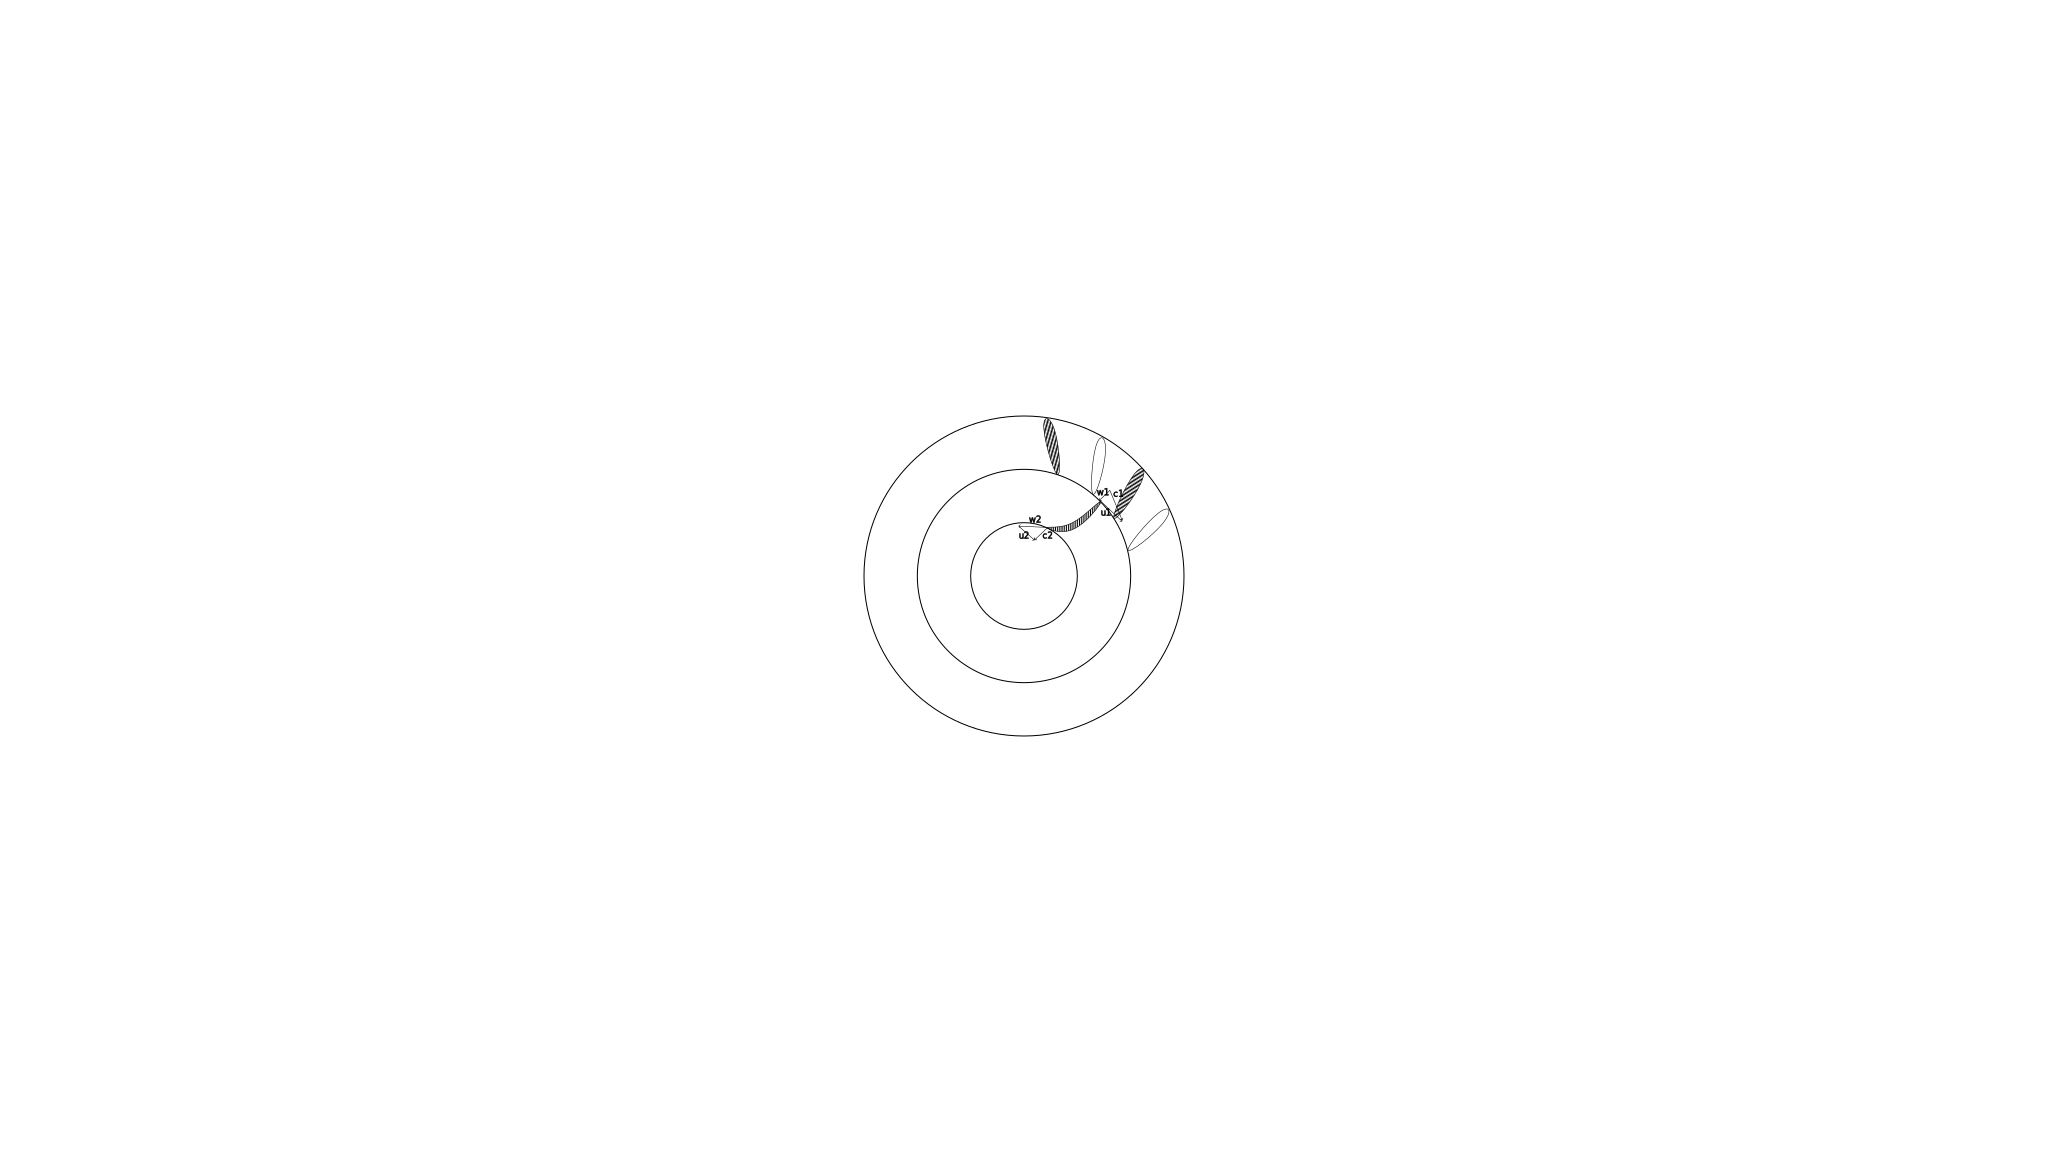
\includegraphics[width=0.7\linewidth]{inkscape/Francis.pdf}
\end{figure}
	Le palette dello statore hanno un profilo neutro. \newline
	
	In ingresso $\alpha_1\leq90\degree$, si può porre tuttavia per semplicità una velocità grossomodo verticale. \newline 
	
	Per massimizzare il lavoro estratto e ottenere un triangolo di uscita sempre valido in condizioni di progetto si passa sempre attraverso la formula del lavoro:
	\[l = \dfrac{c_1^2-c_2^2}{2} + \dfrac{P_1-P_2}{\rho}\]	
	Dal punto di vista del rotore la differenza di entalpia risulta tuttavia fissata, si può allora fare in modo che il contributo $c_2^2$ diminuisca, questo è infatti pari a:
	\[c_2^2 = c_{2m}^2 + c_{2u}^2\]
	Mentre la componente meridiana è bloccata dalla portata in ingresso, si può agire sulla componente $c_{2u}$ facendola ipoteticamente tendere allo zero, condizione che si verifica se e soltanto se $c_2\perp u_2$. \newline 
	
	Ricapitolando, i triangoli di velocità funzionalmente corretti ad un determinato $\Delta P$ si ottengono sotto le seguenti condizioni:
	\begin{enumerate}
		\item \(u_1>u_2\)
		\item \(c_{1u}>c_{2u}\)
		\item \(|w_2|>|w_1|\)
	\end{enumerate}
	Se d'altra parte si sceglie di operare con una $c_{2u}<0$, il lavoro certamente cresce, ma per ottenere una componente tangenziale così marcata e quindi accelerare maggiormente il flusso, servirebbe un maggiore $\Delta P$ e quindi un rotore più grande 
\end{adjustwidth}
		
		

\subsection{Rendimento di palettatura}
\begin{adjustwidth}{2in}{}
	In condizioni di progetto, quinci con $c_{2u}=0$, si ottiene:
	\[\eta = {l\over gH_u} = \dfrac{u_1c_{1u}}{gH_u}\]
	Dato un generico triangolo di velocità si può scrivere:

	\begin{tikzpicture}[>=latex] [font=\itshape]
%	\draw [help lines] (0,0) grid (5,5);
	\draw [->] (2,1) -- (5,1) node  [pos=0.5, sloped, below] {$u_1$};
	\draw [->] (0,4) -- (5,1) node  [pos=0.5, sloped, above] {$c_1$};
	\draw [->] (0,4) -- (2,1) node  [pos=0.5, sloped, above] {$w_1$};
	\draw [->] (1.5,1) arc (180:150:1) node  [pos=0.5, sloped, above] {$\beta_1$};
	\draw [dashed] (2,1) -- (1.5,1);
	\draw [->] (4,1) arc (180:150:1) node  [pos=0.5, sloped, above] {$\alpha_1$};
	\draw [->] (0, 0.5) -- (5, 0.5) node  [pos=0.5, sloped, below] {$c_{1u}$};		
\end{tikzpicture}

	\[c_{1u} = c_1\cos\alpha_1\]
	E quindi:
	\[\eta = \dfrac{u_1c_1\cos\alpha_1}{gH_u}\]
	L'unico parametro lavorabile per aumentare il rendimento di palettatura è l'angolo di ingresso $\alpha_1$, questo infatti dovrà essere piccolo, in questo modo sarà maggiore la componente tangenziale del flusso, ma non troppo piccolo da "annullare" la portata. \newline 
	
	Si sceglie così
	\[\alpha_1 = (10\div20)\degree\]
	
\end{adjustwidth}		


\newpage

\subsection{Grado di reazione}
\begin{adjustwidth}{2in}{}
	Essendo la turbina Francis una macchina a reazione ci si aspetta un grado di reazione $R$ sicuramente positivo e non nullo, non esiste tuttavia una regola generale per individuare a priori il grado di reazione di una turbina di questo tipo, generalmente se ne ottiene il valore alla fine, a posteriori. \newline 
	
	Ciononostante rimane possibile determinare simbolicamente {\footnotesize $(c_2\ll c_1)$} un ordine di grandezza del grado di reazione. 
	
	Questo infatti era pari a:
	\[\begin{split}
		R = \dfrac{P_1-P_2}{\rho g H_u} = \dfrac{l}{gH_u}-\dfrac{c_1^2-c_2^2}{2gH_u} \approx \\ 
		\approx \eta - \dfrac{c_1^2}{2gH_u} = \eta - \dfrac{\eta c_1^2}{2l} = \eta\left(1-\dfrac{c_1^2}{2c_1u_1\cos\alpha_1}\right) 
	\end{split} \]
	Se, come da ipotesi $\alpha_1\rightarrow0\Rightarrow\cos\alpha_1\rightarrow0$, in più $c_1\approx u_1$:
	
\begin{tikzpicture}[>=latex] [font=\itshape]
%	\draw [help lines] (0,0) grid (5,5);
	\draw [->] (2,1) -- (5,1) node  [pos=0.5, sloped, below] {$u_1$};
	\draw [->] (1,1.3) -- (5,1) node  [pos=0.5, sloped, above] {$c_1$};
	\draw [->] (1,1.3) -- (2,1) node  [pos=0.5, sloped, below] {$w_1$};		
\end{tikzpicture}
	
	E quindi:
	\[R = \eta\left(1-\dfrac{\cancel{u_1^2}}{2\cancel{u_1^2}}\right)\Rightarrow R = {1\over2}\eta\]
	Infine se:
	\[\eta = 1 \Rightarrow R = {1\over2}\]
	Tanto più le ipotesi {\footnotesize $(c_2\downarrow, \alpha_1\downarrow)$} conducono ad un rendimento maggiore, tanto più ci si aspetta un grado di reazione prossimo a $0.5$. 
	
	Se poi ci si pone nelle condizioni in cui $R\gg0.5$ ci si dovrà aspettare un rotore da una palettatura che devii ancor più maggiormente il flusso, ma a questo punto si incorrerebbe in perdite di carico nel rotore non auspicabili. 
\end{adjustwidth}
	
	
	
\subsection{Tubo Diffusore}
\begin{adjustwidth}{2in}{}	
	\begin{tikzpicture}[>=latex] [font=\itshape]
%	\draw [help lines] (0,0) grid (7,7);
	%Monte
	\fill[cyan!30!white] (0,5) rectangle (2,6);
	\node at (1,5.5) {Monte};
	%Turbina
	\node [draw, circle] at (6,4) {T};
	%Valle
	\fill[cyan!30!white] (5,1) rectangle (7,2);
	\node at (6,1.5) {Valle};
	%Collegamenti
	\draw (1,5) to[looseness=.7,bend right=10] (5.65,4);
	\draw (6,3.65) -- (6,2)node  [pos=0.5, right] {Tubo~Diffusore};
	%Asse
	\draw [->] (-1,1) -- (-1,6) node [pos=1, above] {$z$};
	%Marker
	\draw (-1.1,3.65) -- (-0.9,3.65);
	\node [align=left] at (-1.4,3.65) {$z_2$};
	\draw (-1.1,2) -- (-0.9,2);
	\node [align=left] at (-1.4,2) {$z_3$};
	%\fill [cyan] (0,4) -- (2,4) -- (2,5) -- (0,5) -- cycle;
\end{tikzpicture}

	\[{P_M\over\rho} + gz_M = {P_2\over\rho}+{c_2^2\over2} + gz_2 + l \qquad P_3 = P_M = P_{\text{atm}}\]
	\begin{equation}{\label{eq:7}}
		\boxed{l = \dfrac{P_{\text{atm}-P_2}}{\rho} + g(z_M-z_2) - {c_2^2\over2}}
	\end{equation}
	Poiché la quota di monte e quella in uscita della turbina sono quote fisse, invariabili ed ininfluenti, gli unici parametri sui quali si può agire sono $P_2$ e $c_2$, intimamente connessi. \newline 
	
	$P_2$ risulta così lavorabile fino al limite di cavitazione, che si ricorda per un liquido a temperatura ambiente essere di circa $100~\text{Pa}$. 
	
\begin{tikzpicture}[>=latex] [font=\itshape]
%	\draw [help lines] (0,0) grid (7,7);
	\draw (0,5) -- (5,7);
	\draw (0,3) -- (5,1);
	\node at (-0.2,4) {2}; 
	\node at (5.2,4) {3};
	\draw [dashed] (0,3) -- (0,5);
	\draw [dashed] (5,1) -- (5,7);
\end{tikzpicture} 

	Poiché inoltre un $\Delta z$ non apporterebbe alcun vantaggio, anzi porterebbe il fluido pericolosamente vicino al limite di cavitazione, si preferisce costruire un tubo diffusore che sia orizzontale piuttosto che verticale.
	\[{P_2\over\rho} + \cancel{gz_2} + {c_2^2\over2} = {P_3\over\rho} +  \cancel{gz_3} + {c_3^2\over2}\]
	Allora:
	\begin{equation}
		\boxed{{P_2\over\rho} = {P_{\text{atm}}\over\rho} - \dfrac{c_2^2-c_3^2}{2}}
	\end{equation}
	Se il fine è quello di ottenere una pressione di scarico dalla turbina minore, si deve necessariamente far uscire il fluido ad una velocità maggiore: $c_2>c_3$. \newline 
	
	Ecco spiegata l'utilità del tubo diffusore, si vede infatti da (\ref{eq:7}) che una diminuzione di $P_2$ al di sotto della pressione atmosferica, permette un aumento del lavoro specifico: si recupera l'energia cinetica allo scarico sotto forma di pressione. 
	
	Esiste tuttavia - come detto - un limite invalicabile, ossia quello della cavitazione, che non permette di recuperare la totalità dell'energia cinetica allo scarico, c'è infatti sempre una componente tangenziale e non perfettamente meridiana e quindi non recuperabile in uscita dalla palettatura, che imprime al fluido nel diffusore un moto vorticoso. 	
\end{adjustwidth}
		
		
		
\subsection{Regolazione della potenza}		
\begin{adjustwidth}{2in}{}
	\[P = \dot{m}l\eta\]
	È noto che le macchine ad azione come la Pelton siano parzializzabili al contrario di quelle a reazione come la Francis e la Kaplan, infatti una parzializzazione di queste turbine porterebbe solo una parte di palettatura ad essere investita dal flusso. 	
	Come si può allora operare sulla potenza, e quindi sulla portata, senza che le palettature della turbina - fisse - subiscano una variazione di flusso? Agendo sulle palettature del distributore, infatti queste sono calettate in modo da essere orientabili. 	
\begin{figure}[H]
	\centering
	\includegraphics[width=0.3\linewidth]{immagini/turbinafrancis4}
	\label{fig:turbinafrancis4}
\end{figure}
	Si può così, inclinando le palette, ridurre la portata diminuendo la sezione di passaggio senza intaccare la velocità del flusso. 
\newpage	
	Cosa succede ai triangoli di velocità? 
	
\begin{tikzpicture}[>=latex] [font=\itshape]
%	\draw [help lines] (0,0) grid (15,5);
	%Triangolo d'ingresso
	\draw [->] (0,0) -- (4,0) node  [pos=0.5, sloped, below] {$u_1$};
	\draw [->] (0,4) -- (0,0) node  [pos=0.25, left] {$w_1$};
	\node [align=left] at (-0.3,1) {$w^*_1$};
	\draw [->] (0,4) -- (4,0) node  [pos=0.5, sloped, below] {$c_1$};
	\draw [->] (0,2) -- (4,0) node  [pos=0.5, sloped, below] {$c^*_1$};
	\node [draw, align=left] at (2,-1) {Diminuire la portata significa\\abbassare l'altezza del triangolo};
	%Triangolo d'uscita 
	\draw [->] (8,0) -- (10,1) node  [pos=0.5, sloped, below] {$u_2$};
	\draw [->] (8,3) -- (8,0) node  [pos=0.75, left] {$w_2$};
	\node [align=left] at (7.7,2) {$w^*_2$};
	\draw [->] (8,3) -- (10,1) node  [pos=0.5, sloped, below] {$c_2$};
	\draw [->] (8,3) -- (11,1.5) node  [pos=0.5, sloped, above] {$c^*_2$};
	\draw [->] (8,1.5) -- (11,1.5) node  [pos=0.5, sloped, below] {$u^*_2$};
	
	\node [draw, align=left] at (9,-1) {Diminuire la portata significa\\che in uscita $c_2^*$ non è più \\ perpendicolare ad $u_2$};	
\end{tikzpicture}

	In ingresso, riducendo l'area di passaggio si fornisce più componente tangenziale a $c_1$; diminuendo la portata si abbassa l'altezza del triangolo mantenendo inalterato $\beta_1$: orientando lo statore si deve poter ridurre la componente $c_m$, questa strettamente legata alla portata. \newline 
	
	In uscita il flusso è sempre determinato dalla palettatura, ma avrà un altezza minore data da una portata in ingresso minore.
	
	Non essendoci palette orientabili internamente al rotore, $c_2$ non riesce più a restare ortogonale a $u_2$ e aumentano le perdite di scarico. \newline 
	
	Come effetto secondario si intacca anche il lavoro specifico: ora esiste una $c_{2u}>0$ che ne comporta una riduzione. 
	
	Questo è tuttavia un risultato da aspettarsi: nelle macchine motrici, come queste in esame, al variare della portata (aumenta) varia il lavoro specifico (diminuisce).	
\end{adjustwidth}		
		
		

\subsection{Cavitazione}
\begin{adjustwidth}{2in}{}
	Problematica da cui è esente la turbina Pelton, sia la Francis che la Kaplan soffrono la cavitazione. 
	
	Sono entrambe dotate di un tubo diffusore che aumenta la pressione all'uscita ma questo non basta, prima di tutto questo deve essere dimensionanto in modo da evitare brusche variazioni di sezione, e poi è sempre necessario verificare la quota d'installazione della macchina attraverso il fattore di cavitazione. \newline 
	
	Mentre le turbopompe cavitano in aspirazione, le turbine cavitano in scarico: si sottrae lavoro al fluido e ci si trova nella zona di minima pressione. 
	
	Nelle turbine si usa un fattore di cavitazione adimensionale simile all'NPSH:
	\[\sigma^* = f(\omega_s)\]
	
	\begin{center}		
	\begin{tabular}{|c|c|c|c|}
		\hline
		 $\omega_s$  & 0.45  &   1   &  2   \\ \hline
		 $\sigma^*$ & 0.025 & 0.115 & 0.48 \\ \hline
	\end{tabular}
	\end{center}

	Si individua la quota di scarico come la differenza tra il pelo libero e la quota di installazione della turbina, in questo modo:
	\[\max(z_{sc}) = \dfrac{P_{\text{atm}} - P_v(T)}{\rho g} - \sigma^*(\omega_s) H_u = [\text{m}]\]
	È possibile, se dai calcoli $H_u\uparrow\Rightarrow z_{sc}<0$, installare la turbina sotto battente idraulico, ma col rischio di aumentare le perdite di carico nel diffusore e di non riuscire a recuperare l'energia cinetica in uscita.
	\begin{figure}[H]
		\centering
		\includegraphics[width=0.3\linewidth]{immagini/turbinafrancis5}
		\caption{Sopra battente}
		\includegraphics[width=0.3\linewidth]{immagini/turbinafrancis6}	
		\label{fig:turbinafrancis5}
		\label{fig:turbinafrancis6}
	\end{figure}
	Il fattore di cavitazione assume così i seguenti equivalenti significati:
	\begin{itemize}
		\item Data una certa macchina, quanto la si può alzare/abbassare per recuperare energia cinetica allo scarico ed evitare la cavitazione?
		\item Limite massimo di giri della macchina al fine di evitare la cavitazione: $\sigma\uparrow~\omega_s\uparrow$
		
		In una macchina veloce l'energia allo scarico è sempre maggiore.		
	\end{itemize}	
\end{adjustwidth}		


\newpage

\section{Turbina Kaplan}		
\begin{adjustwidth}{2in}{}
	Le turbine Kaplan sono usate per elaborare grandi portate $100~\nicefrac{\text{m}^2}{\text{s}}$ sotto piccoli salti motore $<30~\text{m}$, per questo usate prevalentemente negli impianti idroelettrici ad acqua fluente. 
	
	Anche questa è una macchina motrice, una turbina a reazione, ha una girante prevalentemente assiale e funzione per velocità specifiche $\omega_s>1.7$ 
	\begin{figure}[H]
		\centering
		\includegraphics[width=0.5\linewidth]{immagini/turbinakaplan3}
		\label{fig:turbinakaplan3}
	\end{figure}	
	A livello costruttivo il flusso incontra una cassa a spirale, poi un distributore palettato regolabile che fornisce componente tangenziale, un rotore palettato dalle palette orientabili ed infine un diffusore: anche con questa tipologia di turbine si deve limitare la perdita di energia cinetica allo scarico. \newline 
	
	Il numero di palette è limitato e compreso tra le 3 e le 8 ma sono di più grandi dimensioni, è una macchina pensata per le alte velocità specifiche; il criterio progettuale è quello di offrire la minima resistenza alla portata che le investe, si limita perciò la superficie di contatto offrendo un canale più lungo dove il flusso possa scorrere. 
	\begin{figure}[H]
		\centering
		\includegraphics[width=0.3\linewidth]{immagini/turbinakaplan4}
		\label{fig:turbinakaplan4}
	\end{figure}
	Poiché la Kaplan è utilizzata negli impianti ad acqua fluente, questi caratterizzati da una importante variabilità di portata annua, devono poter regolare la portata sia attraverso lo statore che attraverso il rotore, in questo modo sia in entrata che in uscita si mantiene un triangolo di velocità ottimizzato. 
\end{adjustwidth}

\newpage

\subsection{Triangoli di velocità e ottimizzazione}
\begin{adjustwidth}{2in}{}
	Dove e come si disegnano i triangoli di velocità in una turbina Kaplan?
	
\begin{figure}[H]
	\centering
	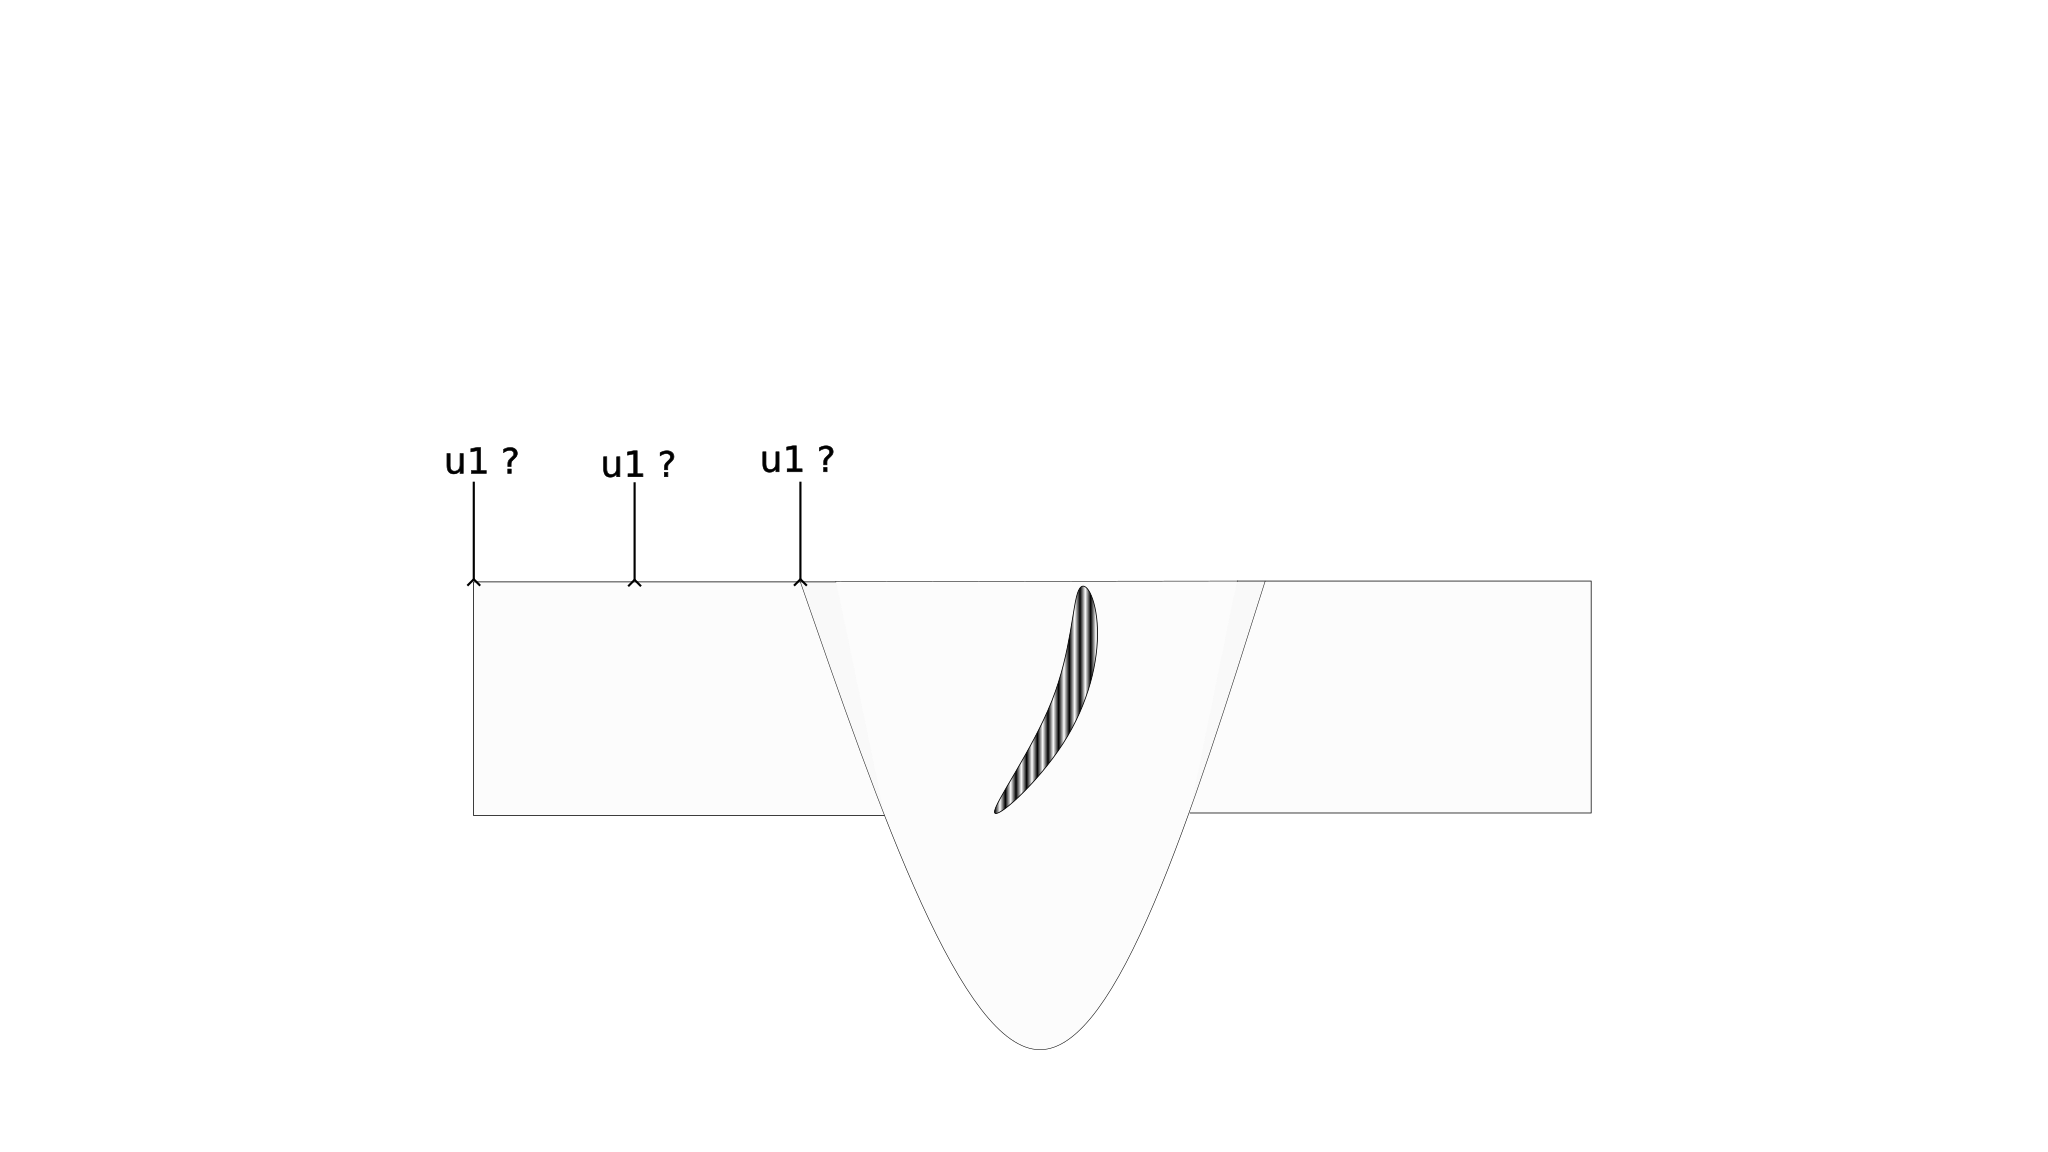
\includegraphics[width=0.7\linewidth]{inkscape/Kaplan1.pdf}
	\label{fig:kaplan1}
\end{figure}

	Al diametro esterno, a quello interno oppure al diametro medio? 
	
	Quest'ultimo generalmente si sottende essere rappresentativo del fenomeno. 
	
	I triangoli di velocità al diametro medio saranno allora: 
	
\begin{tikzpicture}
	%\draw [help lines] (0,0) grid (10,10);
	%Palettatura
	\draw [thick] (7,7) to [out=225, in=35] (3,3);
	%Triangolo in ingresso
	\draw [->] (6,8) -- (8,8) node [pos=0.5, sloped, above] {$u$};
	\draw [->] (8,8) -- (7,7) node [pos=0.5, sloped, below] {$w_1$};
	\draw [->] (6,8) -- (7,7) node [pos=0.5, sloped, below] {$c_1$};
	%Triangolo in uscita 
	\draw [->] (1,3) -- (3,3) node [pos=0.5, sloped, above] {$u$};
	\draw [->] (3,3) -- (1,2) node [pos=0.5, sloped, below] {$w_2$};
	\draw [->] (1,3) -- (1,2) node [pos=0.5, left] {$c_2$};
\end{tikzpicture}

	Il condotto è sempre accelerante $u_1=u_2=u$: la macchina è pur sempre assiale.
	\[l = \dfrac{c_1^2-c_2^2}{2} - \dfrac{w_1^2-w_2^2}{2} + \cancel{\dfrac{u_1^2-u_2^2}{2}}\]
	L'unico termine che contribuisce alla variazione di pressione è quello della velocità relativa $w$. \newline 
	
	Si nota subito che la turbina Kaplan è adatta a impieghi dal basso lavoro specifico, dall'elevata portata e dai salti motore contenuti. \newline 
	
	Come nella turbina Francis, valgono:
	\[l = c_{1u}u_1 = c_1u_1\cos\alpha_1\qquad\eta=\dfrac{c_1u_1\cos\alpha_1}{gH_u}\]
\end{adjustwidth}

\newpage

\subsection{Particolarità}
\begin{adjustwidth}{2in}{}
	Il profilo della palettatura è diverso tra l'apice e la base in virtù della velocità di rotazione. 
	
\begin{figure}[H]
	\centering
	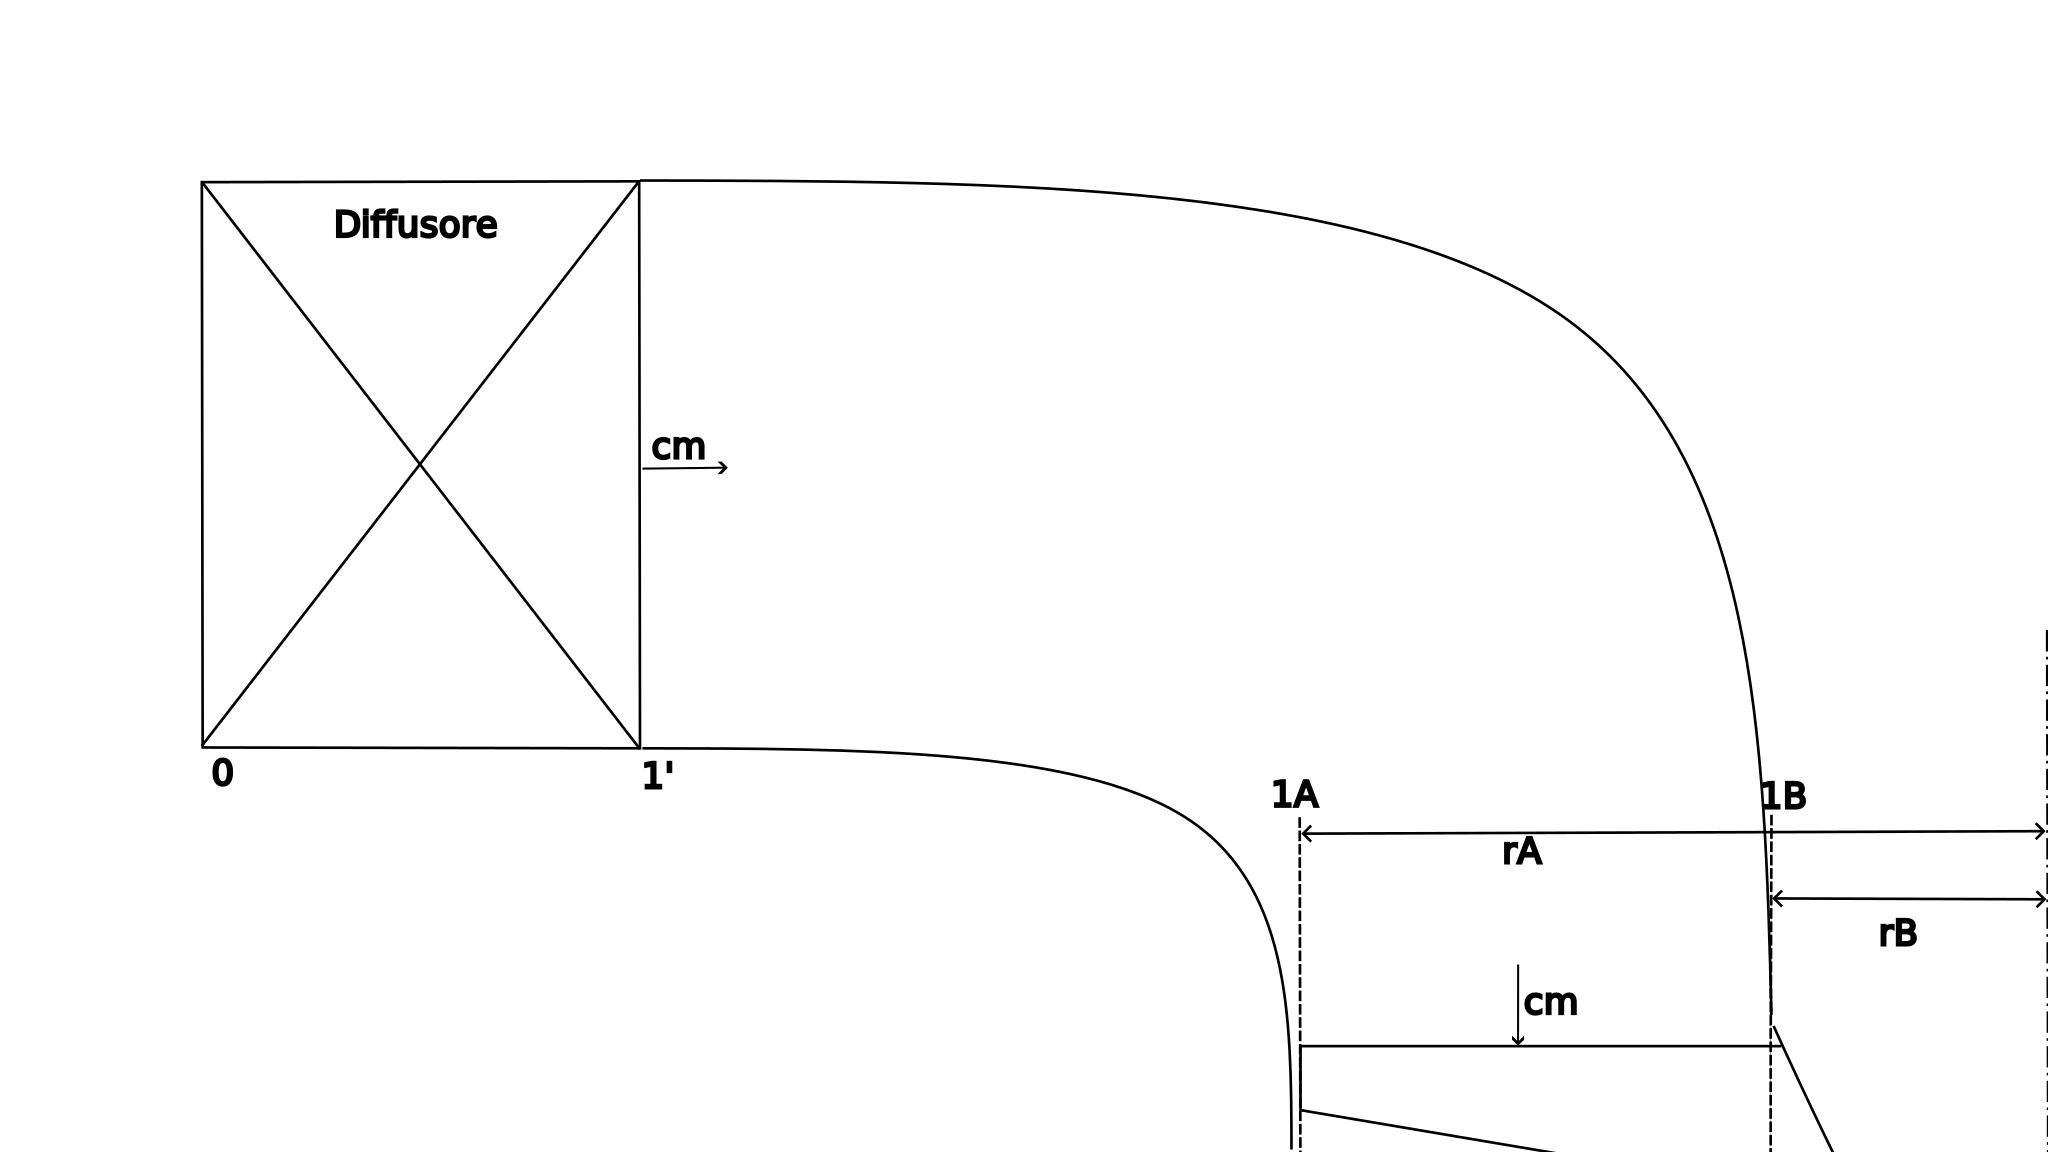
\includegraphics[width=0.7\linewidth]{inkscape/Kaplan2.pdf}
	\label{fig:kaplan2}
\end{figure}

	\begin{center}
		\begin{tabular}{|c|c|c|}
		\hline
		       Apice         &   &         Base         \\ \hline
		  $u_A=\omega r_A$   & > &   $u_B=\omega r_B$   \\ \hline
		      $c_{mA}$       & = &       $c_{mB}$       \\ \hline
		$\Gamma_A=r_Ac_{uA}$ & = & $\Gamma_B=r_Bc_{uB}$ \\ \hline
	\end{tabular}
	\end{center}

\vspace{0.5cm}
	È quest'ultima uguaglianza a definire la particolarità della turbina Kaplan, infatti il flusso appena uscito dal distributore raggiunge il rotore dopo aver percorso un angolo di 90\degree, in quel tragitto, non essendoci pale fisso o mobili a cambiare il momento angolare $\Gamma$ del fluido, questo si conserva e permette di dimostrare che:
	\[c_{uA}<c_{uB}\]
	Il lavoro che estrae la pala all'apice è pari a
	\[l_A = u_Ac_{1uA} = \omega r_Ac_{1uA}\]
	Il lavoro che estrae la pala alla base è:
	\[l_B = u_Bc_{1uB} = \omega \cancel{r_B}r_A{c_{1uA}\over \cancel{r_B}} = \omega r_Ac_{1uA}\]
	Esattamente uguale al lavoro che estrae la pala all'apice, che è uguale al lavoro totale estratto. 
\end{adjustwidth}	
	\begin{tikzpicture}[>=latex] [font=\itshape]
	%\draw [help lines] (0,0) grid (15,5);
	\draw [->] (0,5) -- (5,5) node [pos=0.5, sloped, above] {$u_{1A}$};
	\draw [->] (0,5) -- (2,0) node [pos=0.5, sloped, below] {$c_{1A}$};
	\draw [->] (5,5) -- (2,0) node [pos=0.5, sloped, below] {$w_{1A}$};
	\draw [->] (10,5) -- (13,5) node [pos=0.5, sloped, above] {$u_{1B}$};
	\draw [->] (10,5) -- (15,0) node [pos=0.5, sloped, below] {$c_{1B}$};
	\draw [->] (13,5) -- (15,0) node [pos=0.5, sloped, below] {$w_{1B}$};
\end{tikzpicture}
\begin{adjustwidth}{2in}{}	
	Il progressivo aumento di sezione dall'apice verso la base per far fronte alla diversa velocità di rotazione con l'obiettivo di mantenere il lavoro costante è chiamata operazione di svergolamento. 
\end{adjustwidth}

\newpage

\part{Turbine Eoliche}

\begin{adjustwidth}{2in}{}
	Le turbine eoliche sono macchine a flusso incomprimibile seppur il fluido utilizzato sia gassoso, è utile infatti ricordarsi che la proprietà di comprimibilità o incomprimibilità dipende dal flusso e non dal fluido; infatti le turbine eoliche, dato che per la velocità del vento $Ma\ll1$, possono essere considerate macchine a flusso incomprimibile perché non avvengono fenomeni di comprimibilità. \newline 
	
	Le turbine eoliche sono usate per la produzione di energia e sono fonti discontinue e non controllabili. \newline 
	
	Se lo studio del vento viene effettuato secondo il modello di lastra piana investita dal flusso è possibile considerare la velocità del vento nota sia nello spazio che nel tempo: l'inurbamento è compreso nello strato limite e la turbina lavora nella zona di flusso indisturbato, a velocità costante.	
	\begin{figure}[H]
		\centering
		\includegraphics[width=0.5\linewidth]{immagini/eoliche13}
		\label{fig:eoliche13}
	\end{figure}	
\end{adjustwidth}



\section{Tipologie di turbine eoliche}
\begin{adjustwidth}{2in}{}
	Le turbine eoliche essendo collegate a generatori in DC non presentano la problematica che si era incontrata con le turbine idrauliche ovvero quella di un alternatore che debba girare alla loro stessa frequenza. \newline 
	
	Le pale di una turbina eolica altro non sono che profili alari.
	\begin{figure}[H]
		\centering
		\includegraphics[width=0.4\linewidth]{immagini/eoliche1}
		\includegraphics[width=0.4\linewidth]{immagini/eoliche2}
		\label{fig:eoliche1}
		\label{fig:eoliche2}
	\end{figure}
	\newpage
	 In passato le pale venivano trascinate dalla resistenza aerodinamica, non funzionavano per lift ma per drag (come avere il vento in poppa).
	 \begin{figure}[H]
	 	\centering
	 	\includegraphics[width=0.5\linewidth]{immagini/eoliche3}
	 	\label{fig:eoliche3}
	 \end{figure}
 	Nel presente, seppur le Drag Wind Turbines rimangano una moderna applicazione di nicchia, le turbine eoliche maggiormente utilizzate sfruttano la portanza, il lift. 
 	\begin{figure}[H]
 		\centering
 		\includegraphics[width=0.3\linewidth]{immagini/eoliche5}
 		\label{fig:eoliche5}
 	\end{figure}
 	Le turbine eoliche possono essere ad asse verticale o ad asse orizzontale
 	\begin{figure}[H]
 		\centering
 		\includegraphics[width=0.5\linewidth]{immagini/eoliche4}
 		\label{fig:eoliche4}
 	\end{figure}	  
\end{adjustwidth}



\subsection{Turbine ad asse verticale}
\begin{adjustwidth}{2in}{}
\begin{figure}[H]
	\centering
	\includegraphics[width=0.5\linewidth]{immagini/eoliche6}
	\label{fig:eoliche6}
\end{figure}
	Sono turbine di dimensioni ridotte adatte allo sviluppo fino ai 10 kW. 
	
	Non necessitano di essere orientate in funzione della direzione del vento e presentano palettature che possono estendersi fino al suolo, adatte principalmente a basse velocità del vento. \newline 
	
	Sono turbine che necessitano di essere avviate e hanno bisogno di una particolare sensoristica che legga la velocità del vento in modo da farle attivare nel loro range di funzionamento. 
	
	Sono macchine che di contro hanno un'elevata fluttuazione della coppia ed una tensione prodotta non costante: le forze si compongono in modo diverso in funzione della posizione delle pale.  
\end{adjustwidth}



\subsection{Turbine ad asse orizzontale}
\begin{adjustwidth}{2in}{}
	\begin{figure}[H]
		\centering
		\includegraphics[width=0.5\linewidth]{immagini/eoliche7}
		\label{fig:eoliche7}
	\end{figure}
	Sono turbine più efficienti ed offrono più superficie al vento e necessitano i meccanismi di rotazione. 
	
	Si possono trovare in formato Upwind (sopravento) o Downwind (sottovento) in funzione di come sono state installate.
	\begin{figure}[H]
		\centering
		\includegraphics[width=0.5\linewidth]{immagini/eoliche8}
		\label{fig:eoliche8}
	\end{figure}
	Come intuibile lavorano per elevate portate di fluido e sono caratterizzate da basso lavoro specifico. 
	
	In questi tipi di turbine non è previsto uno statore per evidenti motivi costruttivi, ma le sue funzioni vengono tuttavia svolnte dal controllo della rotazione della navicella e dall'angolo di attacco delle pale. 
\end{adjustwidth}

\newpage

\section{Dimensionamento del parco eolico}
\begin{adjustwidth}{2in}{}
	Poiché l'installazione di un parco eolico è estremamente costosa 3000\$ per kW installato, sono necessari attenti e minuziosi studi di fattibilità. \newline 
	
	Si parte in prima battuta dall'analisi della curva caratteristica della turbina che si vuole installare:
	\begin{figure}[H]
		\centering
		\includegraphics[width=0.5\linewidth]{immagini/eoliche9}
		\label{fig:eoliche9}
	\end{figure}
	Si identifica una velocità di out-in o di ingresso per la quale la pala non viene messa in moto, è economicamente sconveniente, ci sarebbero più perdite che guadagni. Il rotore gira, ma non è in
	grado di generare corrente.
	
	Si identifica una velocità di out-out o cut-off per la quale la pala viene bloccata, le velocità eccessive a cui verrebbe sottoposta rischierebbero il suo danneggiamento. 
	
	Si identifica poi la potenza nominale come il valore corrispondente alla velocità nominale $(10\div15~\nicefrac{\text{m}}{\text{s}})$, condizione prossima a quella in cui la turbina inizia ad andare in sicurezza e a
	limitare l’output. La generazione della potenza nominale è ciò che ci si deve aspettare dal corretto dimensionamento di una turbina eolica.
	
	La potenza di picco rappresenta invece la massima
	potenza che la turbina può generare. Un valore
	elevato della potenza di picco non costituisce
	necessariamente un fattore di pregio, in quanto
	si verifica raramente in presenza di venti forti. \newline 
	
	Identificata la tipologia di turbina che andrà a comporre il parco eolico, sarà ora necessario analizzare in prima approssimazione dei database di venti e e poi dei grafici di densità di probabilità (PDF) per determinare per quanto tempo permane quella specifica velocità del vento.
	\begin{figure}[H]
		\centering
		\includegraphics[width=0.5\linewidth]{immagini/eoliche10}
		\label{fig:eoliche10}
	\end{figure}
	In ascissa sono riportati i valori di velocità del
	vento mediati su una durata di 10 minuti.
	
	Per ogni valore di velocità la curva riporta il
	tempo di permanenza complessiva misurato nel
	corso dell’anno, in percentuale oppure in ore.
	
	Ai fini del calcolo della resa energetica annua, la
	curva di distribuzione va confrontata con la curva
	di potenza della turbina. \newline 
	
	
	La producibilità annua può essere espressa attraverso la seguente formulazione:
	\[E = 8760\cdot\eta\cdot\int_{0}^{u_{\max}}P(u)\cdot\text{PDF}(u)\cdot du\]
	In cui: 
	\begin{itemize}
		\item $\eta$ è il rendimento dell'impianto
		\item $P(u)$ è la potenza in kW prodotto dalla turbina alla velocità del vento dedotta dalla curva di potenza fornita dal costruttore
		\item $\text{PDF}(u)$ è la funzione di distribuzione di probabilità (Probability Dense Function) di frequenza delle velocità del vento nel sito d'installazione. 
		\item $8760$ è un semplice fattore di conversione, è il numero delle ore in un anno. 
	\end{itemize}
	
	\vspace{0.5cm}
	Sarà quindi necessario valutare in modo puntuale se la
	maggiore resa in condizioni di vento forte
	compensa la perdita di resa con venti più deboli
	rispetto ad una turbina di potenza nominale
	meno elevata e, probabilmente, meno
	costosa. \newline 
	
	Se la stima preliminare è fruttuosa si procederà con misurazioni in situ per almeno 12/18 mesi. 
\end{adjustwidth}



\subsection{Posizionamento dell'aerogeneratore}
\begin{adjustwidth}{2in}{}
	Stabilita la zona di installazione, per un corretto
	posizionamento dell’aerogeneratore bisogna
	considerare la presenza di eventuali ostruzioni
	geologiche e non, quali alberi o edifici, che
	possano generare turbolenze e determinare una
	perdita di produttività dell’impianto. \newline 
	
	Come già anticipato, si vuole che l'impianto lavori in regime di velocità costante e di flusso indisturbato, quindi all'esterno dello stato limite. 
	\begin{figure}[H]
		\centering
		\includegraphics[width=0.5\linewidth]{immagini/eoliche11}
		\label{fig:eoliche11}
	\end{figure}	
	Per determinare il profilo di velocità del vento in funzione
	della quota si può utilizzare questa relazione
	\[ c = c_0\left(h\over h_0\right)^\alpha\]
	Che consente
	di ricavare la velocità del vento $c$ alla quota $h$ di installazione della navicella, note che
	siano la velocità $c_0$ alla quota $h_0$, magari da rilievi anemometrici,
	e la rugosità del terreno $\alpha$:
	
	\begin{tabular}{|c|c|}
		\hline
		 $\alpha=0.9$   &      mare calmo      \\ \hline
		 $\alpha=0.12$  & aree agricole aperte \\ \hline
		$\alpha = 0.30$ & zone urbane, boschi  \\ \hline
	\end{tabular}
	\begin{figure}[H]
		\centering
		\includegraphics[width=0.3\linewidth]{immagini/eoliche12}
		\label{fig:eoliche12}
	\end{figure}	
	Per quanto possibile, è buona norma cercare di prevedere
	la costruzione di nuovi edifici oppure la
	crescita di alberi esistenti, visto che la durata in
	servizio del sistema può raggiungere i 20 anni.
	
	Come regola generale, la turbina va posizionata
	sopravento ad edifici e alberi e dovrebbe essere
	almeno 10m più elevata di qualunque altra cosa
	nel raggio di 100m.
	La presenza di un edificio determina infatti una
	forte turbolenza nella zona sottovento, che si
	estende su una lunghezza che può arrivare fino a
	20 volte l’altezza dell’edificio stesso.
\end{adjustwidth}



\section{Potenza estratta}

\begin{adjustwidth}{2in}{}
	Data una pala di un certo diametro, quanta energia è possibile estrarre? \newline 
	
	Per rispondere a questa domanda si passa attraverso lo studio di un modello semplificato di tubo di flusso, si considera cioè il rotore come un disco piano infinitesimo di area $A$ investito da un flusso in direzione $x$ ad una certa velocità $c_{x1}$. 
	\begin{figure}[H]
		\centering
		\includegraphics[width=0.3\linewidth]{immagini/eoliche14}
		\label{fig:eoliche14}
	\end{figure}
	Alla sezione di ingresso 1 si pone il fluido essere insubordinato, non risente della presenza della pale, all'uscita il flusso potrà porsi sempre indisturbato, è stato cambiato dalla presenza delle pale ma è molto distante e non risente più della loro influenza. 
	
	Poiché la pala estrae energia, ci si aspetta $c_{x3}<c_{x1}$ mentre $P_1=P_3=P_{\text{atm}}$, inoltre $A_1=A_2\ne A_3$
	\begin{figure}[H]
		\centering
		\includegraphics[width=0.5\linewidth]{immagini/eoliche15}
		\label{fig:eoliche15}
	\end{figure}
	La portata che investe le pale è: 
	\[\dot{m} = \rho c_{x2}A_2\]
	Effettuando il bilancio della quantità di moto tra le sezioni 1 e 3 si scopre come effettivamente agisca una forza: 
	\[F_x = \dot{m}c_{x1} - \dot{m}c_{x3} = \dot{m}(c_{x1}-c_{x3})\]
	La potenza diviene così pari a 
	\[P = F_xc_{x2} = \dot{m}c_{x2}(c_{x1}-c_{x3})\]
	Sostituendo la formulazione della portata si ottiene 
	\begin{equation}{\label{eq:8}}
		P = \rho A_2c^2_{x2}(c_{x1}-c_{x3})
	\end{equation}
	Si ottiene in questo modo la potenza scambiata dalla pala grazie alla corrente fluida, il problema però è che rimane incognito il termine $c_{x3}$. \newline 
	
	Ci si accorge allora che la potenza può essere calcolabile anche come quantità di energia sottratta alla corrente fluida, infatti
	\[\begin{cases}
	\begin{aligned}
			P_{W1} &= \dot{m}{c_{x1}^2\over2} \\
		P_{W3} &= \dot{m}{c_{x3}^2\over2}	
	\end{aligned}
	\end{cases}\Rightarrow \Delta P_{W} = \dot{m}\left({c_{x1}^2\over2}-{c_{x3}^2\over2}\right)\]
	Si ritrova l'energia cinetica del vento come energia estratta dalle pale; il problema anche qui  è che $c_{x3}$ continua ad essere incognito.  \newline 
	
	Si sfrutta allora il fatto che le due potenze ricavate devono essere uguali, ovvero l'energia sottratta al vento $P_W$ deve essere pari a quella scambiata dalle pale $P$, allora
	\[P_W = P\]
	\[{\cancel{\dot{m}}\over2}(c_{x1}^2-c_{x3}^2) = \cancel{\dot{m}}c_{x2}(c_{x1}-c_{x3})\]
	\[\cancel{(c_{x1}-c_{x3})}(c_{x1}+c_{x3}) = 2c_{x2}\cancel{(c_{x1}-c_{x3})} \]
	\[c_{x2} = {1\over2}(c_{x1}+c_{x3})\]
	Si trova come primo risultato che la velocità del flusso che investe la pala è la media tra le velocità di ingresso e di uscita, essendo la potenza funzione di questa velocità, risulta proprio da questa limitata. 
	
	Come secondo risultato, ci si può ricavare $c_{x3}$ finora rimasto incognito, infatti: 
	\[c_{x3} = 2c_{x2}-c_{1}\]
	Che sostituita in (\ref{eq:8}) porta a
	\[P = \rho A_2c^2_{x2}(c_{x1}-2c_{x2}+c_{1}) = 2\rho A_2c^2_{x2}(c_{x1}+c_{x2})\]
	Si definisce $a$ Fluid Riduction Coefficient o fattore d'interferenza
	\[a = \dfrac{c_{x1}-c_{x2}}{c_{x1}}\]
	Come la percentuale di riduzione di quantità di moto tra ingresso ed uscita, allora 
	\[c_{x2} = c_{x1}(1-a)\]
	E quindi
	\[P = 2\rho A_2c^2_{x1}(1-a)^2c_{x1}a\]
	Infine 
	\begin{equation}
		\boxed{P = 2\rho A_2 c_{x1}^3a(1-a)^2}
	\end{equation}
	La potenza dipende perciò principalmente dall'area delle pale e dal cubo della  velocità del vento, se nel primo caso si può sopperire con un effettivo aumento delle dimensioni delle pale, per il secondo e più importante fattore, è necessario scegliere con cura la zona di installazione dell'impianto. 
	\begin{figure}[H]
		\centering
		\includegraphics[width=0.5\linewidth]{immagini/eoliche16}
		\label{fig:eoliche16}
	\end{figure}	
\end{adjustwidth}



\subsection{Studio della potenza, Legge di Betz}
\begin{adjustwidth}{2in}{}
	È possibile effettuare uno studio della potenza, e specialmente del termine $a(1-a)^2$ attraverso il coefficiente di potenza $C_P$, questo esprime quanto effettivamente si sta estraendo dalla turbina ed è definito come
	\[C_P=\dfrac{\text{Potenza Ottenuta}}{\text{Potenza Disponibile}} = \dfrac{P}{{1\over2}c^2_{x1}\rho A_1 c_{x1}} = \dfrac{2\rho A_2 c_{x1}^3a(1-a)^2}{{1\over2}\rho A_2 c_{x1}^3} = 4a(1-a)^2\]
	Il massimo del coefficiente di potenza, ovvero il massimo del lavoro estratto, si trova imponendo: 
	\[{d\over da}C_P = 4(3a^2-4a+1)=0 \Leftrightarrow 3a^2-4a+1=0\]
	Che porta all'individuazione di due radici reali distinte
	\[a_1 = 1\qquad a_2 = {1\over3}\]
	Che sostituite all'interno del coefficiente di pressione portano a
	\[C_P(1) = 0 \qquad C_P\left(1\over3\right)\approx0.593\]
	Ciò significa che il massimo lavoro estraibile da una turbina eolica raggiunge a mala pena il 60\% dell'energia totale del vento. 
	
	Tale risultato va sotto il nome di legge di Betz.
\end{adjustwidth}







\newpage




\part{Turbine a flusso comprimibile o Macchine termiche}
\begin{adjustwidth}{2in}{}
	Le turbine a flusso comprimibile sono principalmente macchine assiali multistadio. 
	\begin{figure}[H]
		\centering
		\includegraphics[width=0.5\linewidth]{immagini/gas1}
		\label{fig:gas1}
	\end{figure}	
	È previsto l'uso di turbine radiali a flusso comprimibile per applicazioni di nicchia a bassissime portate come i turbocompressori per automobili; queste in particolare sono caratterizzate da un elevato lavoro specifico ed una bassissima velocità specifica.\newline 
	
	Nelle turbine a flusso comprimibile diventano significative sia le variazioni di densità che di temperatura del fluido, infatti essendo la velocità dello stesso paragonabile a quella caratteristica, diventa $\rho = f(P)$ col risultato che ora una variazione di entalpia non si porta più solo appresso una variazione di pressione, ma anche di temperatura. \newline 
	
	Il fluido utilizzato è unicamente gassoso: aria, vapore d'aria o gas combusti. 
	\begin{figure}[H]
		\centering
		\includegraphics[width=0.5\linewidth]{immagini/gas2}
		\label{fig:gas2}
	\end{figure}
	Le macchine assiali di maggior utilizzo sono caratterizzate da un'elevata velocità specifica, da un basso lavoro specifico e da un'elevatissima portata. \newline 
	
	Il dimensionamento non si fa più attraverso un diagramma di Baljè valido per ogni macchina, ma dato che i numeri adimensionali salgono a 3 $\Phi, \Psi, Ma$, si usa un diagramma di Baljè a $Ma$ fissato, con l'accortezza che, quando $Ma=1$ il flusso diventa transonico e sarà necessario cambiare geometria alle palette. 
\end{adjustwidth}


\newpage


 \section{Principali applicazioni}
\begin{adjustwidth}{2in}{}
	\begin{itemize}
		\item Impianti a vapore, espansori, ciclo Hirn/Rankine
		\begin{figure}[H]
			\centering
			\includegraphics[width=0.4\linewidth]{immagini/hirn2}
			\includegraphics[width=0.4\linewidth]{immagini/hirn}
			\label{fig:hirn2}
			\label{fig:hirn}
		\end{figure}
	NB: esagera l'altezza del punto 3, il massimo della campana di Andrews per l'acqua è circa 370\degree C, il punto 3 si trova a più di 500\degree C (parola di Facci)
		\[\begin{cases}
			\Delta h \approx 1500~\nicefrac{\text{kJ}}{\text{kg}} \\
			\dot{m} \approx 100\div500~\nicefrac{\text{kg}}{\text{s}}
		\end{cases}\]
	Con la dovuta cautela (c'è sono un termine cinetico a differenza), si può porre
	\[\Delta h \approx l \approx u^2 \Rightarrow u \approx \sqrt{\Delta h} >1000~\nicefrac{\text{m}}{\text{s}}\]
	Una turbina che gira così veloce è impossibile da realizzare, si deve per forza parzializzare, ecco così che diventano necessari più stati che si ripartiscano le velocità. 
	
	\item Impianti turbogas, ciclo Joule-Brayton 
	\begin{figure}[H]
		\centering
		\includegraphics[width=0.4\linewidth]{immagini/BJ}
		\includegraphics[width=0.4\linewidth]{immagini/BJ2}
		\label{fig:BJ}
		\label{fig:BJ2}		
	\end{figure}
	NB: anche qui, parola di Facci, esagera l'altezza della trasformazione 34. 
	\[\begin{cases}
		\beta = {P_2\over P_2} = 15\div30~\text{Rapporto di compressione}\\
		\Delta h \approx 700\div800~\nicefrac{\text{kJ}}{\text{kg}} \Rightarrow u \approx 800~\nicefrac{\text{m}}{\text{s}} \\
		\dot{m} \approx 100~\nicefrac{\text{kg}}{\text{s}}
	\end{cases}\]
	Anche in questo caso è obbligatorio frazionare con una macchina multistadio. 
	
	\item Turbocompressori, Motori a Combustione Interna
	\[\begin{cases}
		\beta = {P_2\over P_2} \approx 2\\
		\Delta h \approx 150~\nicefrac{\text{kJ}}{\text{kg}} \Rightarrow u \approx 400~\nicefrac{\text{m}}{\text{s}} \\
		\dot{m} \approx 0.1~\nicefrac{\text{kg}}{\text{s}}
	\end{cases}\]
	In questo caso, per portate piccole e velocità relativamente basse (la macchina gira comunque molto velocemente) è possibile usare una turbina monostadio radiale. 
	\end{itemize}
\end{adjustwidth}



\section{Analisi Termodinamica}
\begin{adjustwidth}{2in}{}
	Rispetto alle macchine idrauliche c'è una differenza di temperatura da dover considerare, non si può pertanto prescinde lo studio di una turbina a flusso comprimibile da uno studio termodinamico. \newline 
	
	Una macchina a flusso comprimibile è formata da stadi successivi, uno stato a sua volta è composto da uno statore e da un rotore. 
	
	Lo statore ha il compito di preparare il flusso all'estrazione del lavoro che avverrà nel rotore, è formato da ugelli acceleranti e sarà lì che il fluido si espanderà: convertendo energia potenziale (in questo caso un $\Delta h$) in energia cinetica fornendo componente tangenziale al flusso; il rotore è invece l'unico elemento atto allo scambio di lavoro. 
	\[0\rightarrow\boxed{\text{STATORE}}\underset{1}{\rightarrow}\boxed{ROTORE}\rightarrow2\]
	Il parametro principale che si vuole calcolare è il lavoro
	\[l = h_{00}-h_{02} = h_{01} - h_{02}\]
	Definito come la differenza di entalpia totale (o di ristagno). \newline
	
	Si ricordi a tal proposito che l'entalpia di ristagno è una proprietà di campo di un flusso ottenuta rallentandolo fino a velocità nulla, ovvero se una corrente avente un'entalpia specifica $h$ e una velocità $c$ (punto A) viene rallentata fino a velocità nulla mediante una trasformazione adiabatica e
	anergodica (punto o), la sua entalpia specifica aumenta della sua energia cinetica specifica $c^2\over2$.
	\begin{figure}[H]
		\centering
		\includegraphics[width=0.3\linewidth]{immagini/entalpia}
		\label{fig:entalpia}
	\end{figure}
	L'entalpia di ristagno inoltre si conserva anche in presenza di fenomeni dissipativi perché rappresenta l'energia totale del sistema, basta infatti che non ci siano scambi di calore o lavoro per mantenere invariata l'entalpia totale. 
\end{adjustwidth}	
\begin{tikzpicture}[>=latex,
	dot/.style = {draw,fill,circle,inner sep=1pt},arrow inside/.style = {postaction=decorate,decoration={markings,mark=at position .55 with \arrow{>}}}
	]
	%\draw [help lines] (0,0) grid (15,15);		
	%\draw[<->] (0,6) node[above right] {$P$} |- (6,0) node[right] {$V$};
	%\draw[->] (0,0) node[above] {$P$} %|- (6,0) node[right] {$V$};
	\draw[->] (0,0) -- (15,0) node [pos=1, right] {$s$};
	\draw[->] (0,0) -- (0,15) node [pos=1, above] {$h$};
	%ISOBARE
	\draw (4,2) to [out=25, in=225] (9,6);
	\node [align=right] at (9.25,6) {$P_2$};
	\draw (4,6) to [out=25, in=225] (9,10);
	\node [align=right] at (9.25,10) {$P_1$};
	\draw (4,9) to [out=25, in=225] (9,13);
	\node [align=right] at (9.25,13) {$P_0$};
	\draw (4,11) to [out=25, in=225] (9,15);
	\node [align=right] at (9.85,15) {$P_{00} = P_{01}$};
	%QUALCHE NODO
	\node[dot] (@00) at (6,12.17) {};
	\node[dot,blue,label={right:$0$}] (@0) at (6,10.17) {};			
	\node[dot,blue,label={right:$1$}] (@1) at (6,7.17) {};
	\node[dot,blue,label={right:$2$}] (@2) at (6,3.17) {};			
	%Valori sulle y
	\draw[dashed] (@00) to (0,12.17) node [left] {$h_{01}^{\text{Re}} = h_{01} = h_{00}$};
	\draw[dashed] (@0) to (0,10.17) node [left] {$h_0$};
	\draw[blue, dashed] (@1) to (0,7.17) node [left] {$h_1$};
	\draw[blue, dashed] (@2) to (0,3.17) node [left] {$h_2$};
	\draw[blue, dashed] (1,5.17) to (0,5.17) node [left] {$h_{02}$};
	%Valori sulle x
	\draw[blue,dashed] (@2) to (6,0) node [below] {$s_1$};
	%Trasformazioni Ideali
	\draw[arrow inside] (@00) to (@0);
	\draw[blue, arrow inside] (@0) to (@1);
	\draw[blue, arrow inside] (@1) to (@2);
	%Velocità
	\draw (1,10.17) -- (1,12.17) node [pos=0.5, right] {$c_0^2\over2$};
	\draw [blue] (1.5,7.17) -- (1.5,12.17) node [pos=0.5, right] {$c_1^2\over2$};
	\draw [blue] (1,3.17) -- (1,5.17) node [pos=0.5, right] {$c_2^2\over2$};
	%Valori Reali
	\node[dot,red,label={right:$1R$}] (@1R) at (7,8) {};
	\node[dot,red,label={right:$2R$}] (@2R) at (8.5,5.5) {};
	%Trasformazioni reali
	\draw[red, arrow inside] (@0) to[looseness=.7,bend right=10] (@1R);
	\draw[red, arrow inside] (@1R) to[looseness=.7,bend right=5] (@2R);
	%Nuovi valori su x e y
	\draw[red, dashed] (@2R) to (0,5.5) node [left] {$h_{2R}$};
	\draw[red, dashed] (@1R) to (0,8) node [left] {$h_{1R}$};
	\draw[red, dashed] (1,7.5) to (0,7.5) node [left] {$h_{02R}$};
	\draw[red, dashed] (@2R) to (8.5,0) node [below] {$s_{1R}$};
	%Velocità 
	\draw [red] (1,5.5) -- (1,7.5) node [pos=0.5, right] {$c_2^2\over2$};
	\draw [red] (2,8) -- (2,12.17) node [pos=0.25, right] {$c_{1R}^2\over2$};
	%Lavoro
	\draw [<->] (12, 12.17) -- (12, 7.5) node [pos=0.5, right] {$l_R$};
	\draw [loosely dotted] (1,7.5) to (12,7.5);
	\draw [loosely dotted] (@00) to (14,12.17);
	\draw [<->] (13, 12.17) -- (13,5.17) node [pos=0.5, right] {$l_I$};
	\draw [loosely dotted] (1,5.17) to (13,5.17);
	\draw [<->] (14, 12.17) -- (14,3.17) node [pos=0.5, right] {$l_{\max}$};
	\draw [loosely dotted] (@2) to (14,3.17);
\end{tikzpicture}
\begin{adjustwidth}{2in}{}
	Dove si è assunto $c_0\approx c_2$, questa è una considerazione pratica: tra ingrasso e uscita della macchina la velocità è totalmente meridiana perché effettivamente non ha senso avere in uscita velocità con altre componenti fuorché quella meridiana; inoltre tra ingresso e uscita la portata massica deve essere la stessa. 
	
	Notare come nel rotore non valga più la conservazione dell'energia perché si stra estraendo lavoro: $h_{00}=h_{01}\ne h_{02}$ \newline 
	
	Si nota immediatamente una discrepanza tra lavoro reale $l_R$ e lavoro ideale $l_I$, si può allora definire un rendimento:
	\[\eta = {l\over l_{\max}}\]
	Come si individua il lavoro massimo? \newline
	
	Dal grafico, il lavoro reale ottenibile è pari a:
	\[ l_R = \left(h_0 + {c_0^2\over2}\right) - \left(h_2+{c_2^2\over2}\right)\]
	Su cosa si può agire per ottenere il lavoro massimo? $h_{00}$ è fissata, è fornita in input dalla camera di combustione o dal generatore di vapore antistante la turbina, in aggiunta anche $h_2=f(P_2)$ è fissata perché $P_2$ è data dall'atmosfera di scarico della turbina, l'unica scelta libera per la massimizzazione del lavoro è operare su $c_2$, ovvero su come è costruita la macchina. \newline 
	
	Le potenziali fonti di perdita invece possono essere:
	\begin{itemize}
		\item Irreversibilità: \(h_{2R}\gg h_2\)
		\item Velocità di scarico: minore è $c_2^2\over2$ e maggiore sarà il lavoro
	\end{itemize}
	Al limite, il lavoro massimo si otterrebbe idealmente attraverso una velocità di scarico nulla $c_2=0$, ma questo significherebbe non riuscire a portare il flusso fuori dalla turbina
	\[l_{\max} = h_{00}-h_2\]
	Poiché è necessario nella realtà smaltire una portata, si definisce il rendimento Total to Static o efficienza di stato isolato la percentuale di energia che è stato possibile convertire in lavoro meccanico rispetto a quella massima a disposizione, ideale
	\begin{equation}{\label{eq:9}}
		\boxed{\eta_{TS}={l\over l_{\max}} = \dfrac{\left(h_0 + {c_0^2\over2}\right) - \left(h^R_2+{{c_2^2}^R\over2}\right)}{h_0 + {c_0^2\over2} - h_2}}
	\end{equation}
	Ciò che cambia tra numeratore e denominatore è la quantità ${{c_2^2}^R\over2}$ e sebbene identifichi una perdita dal punto di vista energetico, non è considerabile come perdita dal punto di vista termodinamico, infatti il flusso possiede ancora una certa energia meccanica, tuttavia se lo stadio è isolato la perdita di energia allo scarico diviene inevitabile; al contrario se lo stadio non è isolato, ovvero se dopo ne segue un altro, diverrà possibile recuperare quell'energia. \newline 
	
	Si definisce l'efficienza di stato intermedio o rendimento Total to Total
	\begin{equation}{\label{eq:10}}
		\boxed{\eta_{TT} = {l\over l_{\text{isoentropico}}} = \dfrac{\left(h_0 + {c_0^2\over2}\right) - \left(h^R_2+{{c_2^2}^R\over2}\right)}{\left(h_0 + {c_0^2\over2}\right) - \left(h_2 + {c_2^2\over2}\right)}}
	\end{equation}
	Si ha sempre:
	\[\eta_{TS}<\eta_{TT}\]
	Questo spiega perché alla turbina idraulica, essendo monostadio, segue sempre un diffusore per recuperare l'energia allo scarico, nelle turbine a flusso comprimibile si usano invece più stadi susseguenti
\end{adjustwidth}



\section{Grado di reazione}
\begin{adjustwidth}{2in}{}
	Il parametro usato per capire che tipo di macchina utilizzare è il grado di reazione, questo è infatti l'unico parametro che permette di distinguere tra le varie famiglie e tipologie di palettatura, quella da utilizzare. 
	
	È un numero adimensionale legato alla forma della palettatura. 
	\[0\rightarrow\boxed{\text{STATORE}}\underset{1}{\rightarrow}\boxed{ROTORE}\rightarrow2\]
	IL grado di reazione è definito come il rapporto del salto entalpico del rotore con il salto entalpico totale
	\begin{equation}{\label{eq:11}}
		\boxed{R = \dfrac{h_1-h_2}{h_0-h_2} \in [0;1)}
	\end{equation}
	Questo è sempre compreso tra 0 ed 1, ed è strettamente minore di 1: se $R=1$ la turbina non scambia lavoro. \newline 
	
	Spesso, potendo confondere $c_0\approx c_2\Rightarrow l = h_0-h_2$ si può scrivere il grado di reazione come
	\begin{equation}{\label{eq:12}}
		\boxed{R = \dfrac{h_1-h_2}{l}}
	\end{equation}
	La quota parte di lavoro che viene dal salto entalpico, ovvero quanta energia cinetica viene convertita in lavoro. \newline
	
	Tale definizione di rendimento permette inoltre di distinguere tra stadi ad azione e stadi a reazione 
	\begin{itemize}
		\item Stadi ad azione
		\[R=0\]
		\[h_1=h_2\]
		Completa separazione tra il compito dello statore (convertire un salto entalpico in energia cinetica) e del rotore (convertire energia cinetica in lavoro). IL rotore non espande.
		\item Stadi a reazione 
		\[R<1\]
		Generalmente 
		\[R=0.5\]
		Se il $\Delta h$ è troppo grande lo si divide equamente tra statore e rotore
		\[h_1-h_2 = h_0-h_1\]
		\[\Delta h_{\text{rot}} = \Delta h_\text{stat}\]
	\end{itemize}		
\end{adjustwidth}



\subsection{Forma della generica palettatura}
\begin{adjustwidth}{2in}{}
	Poiché $h_2<h_1\Rightarrow w_2>w_1$, il flusso espande, inoltre $u_1=u_2$, allora si può scrivere
	\begin{equation}\label{eq:24}
		\boxed{l = u(c_{1u}-c_{2u})}
	\end{equation}
	Si può a questo punto mettere in relazione il santo entalpico con le velocità relative attraverso Bernoulli applicato al sistema di riferimento relativo, al rotore, dove la componente di trascinamento è uguale e identica
	\[h_1 + {w_1^2\over2} + \cancel{{u_1^2\over2}} = h_2 + {w_2^2\over2} + {\cancel{u_2^2\over2}} \Rightarrow h_1-h_2 = \dfrac{w_2^2-w_1^2}{2}  \]
	In questo modo (\ref{eq:12}) si può scrivere 
	\begin{equation}{\label{eq:13}}
		\boxed{R = \dfrac{w_2^2-w_1^2}{2u(c_{1u}-c_{2u})}}
	\end{equation}
	Scomponendo le velocità relative si ottiene 
	\[R = \dfrac{(w_{2m}^2 + w_{2u}^2) - (w_{1m}^2 + w_{1u}^2)}{2u(c_{1u}-c_{2u})}\]
	Sotto l'ipotesi di validità della conservazione della portata, la componente meridiana ha il solo scopo di trasportare il fluido, per cui: $w_{1m} = w_{2m}$ e allora 
	\[R = \dfrac {w_{2u}^2 - w_{1u}^2}{2u(c_{1u}-c_{2u})}\]
	\[R = \dfrac{(w_{2u}-w_{1u})(w_{2u}+w_{1u})}{2u(c_{1u}-c_{2u})}\]
	Il grado di reazione si manifesta essere una combinazione delle componenti tangenziali.
	
	Ricordando che \(\begin{cases}
		c_{1u} = w_{1u} + u\\
		c_{2u} = w_{2u} + u\\
	\end{cases}\) si può scrivere
	\[R = \dfrac{(w_{2u}-w_{1u})(w_{2u}+w_{1u})}{2u(w_{1u} + u -w_{2u} - u)} = \dfrac{(w_{2u}-w_{1u})(w_{2u}+w_{1u})}{2u(w_{1u} -w_{2u})}\]
	E quindi
	\[R = \dfrac{w_{2u}+w_{1u}}{2u}\]
	Sebbene questa formula così ottenuta sia di scarsa applicazione pratica, infatti generalmente viene utilizzata la (\ref{eq:13}), giustifica a livello teorico la forma della palettatura. 
	
	\begin{tikzpicture}
		%\draw [help lines] (0,0) grid (10,10);
		%Palettatura
		\draw [thick] (7,7) to [out=-15, in=15] (5,1);
		%Triangolo in ingresso
		\draw [->] (7,7) -- (10,7) node [pos=0.5, sloped, below] {$u$};
		\draw [->] (6,8) -- (7,7) node [pos=0.5, sloped, below] {$w_1$};
		\draw [->] (6,8) -- (10,7) node [pos=0.5, sloped, above] {$c_1$};
		%Triangolo in uscita 
		\draw [->] (3,0) -- (6,0) node [pos=0.5, sloped, below] {$u$};
		\draw [->] (5,1) -- (3,0) node [pos=0.5, sloped, above] {$w_2$};
		\draw [->] (5,1) -- (6,0) node [pos=0.5, sloped, above] {$c_2$};
	\end{tikzpicture}
	
%	Tanto il grado di reazione diminuisce, tanto più il flusso sarà deviato.
%	
%	\begin{tikzpicture}
%		%\draw [help lines] (0,0) grid (10,10);
%		%Palettatura
%		\draw [thick] (5,7) to [out=0, in=0] (5,3);
%		%Triangolo in ingresso
%		\draw [->] (3,7) -- (5,7) node [pos=0.5, sloped, below] {$w_1$};
%		
%		%Triangolo in uscita 
%		\draw [->] (5,3) -- (3,3) node [pos=0.5, sloped, below] {$w_2$};
%	\end{tikzpicture}	
\end{adjustwidth}

\newpage

\section{Stadio ad azione semplice Rateau}
\begin{adjustwidth}{2in}{}
	Lo stadio Rateau è una turbina a flusso comprimibile caratterizzata da $R=0$
	\[0\rightarrow\boxed{\text{STATORE}}\underset{1}{\rightarrow}\boxed{ROTORE}\rightarrow2\]
	\[h_1=h_2\]	
\end{adjustwidth}
	\begin{tikzpicture}[>=latex,
	dot/.style = {draw,fill,circle,inner sep=1pt},arrow inside/.style = {postaction=decorate,decoration={markings,mark=at position .55 with \arrow{>}}}
	]
	%\draw [help lines] (0,0) grid (15,15);		
	\draw[->] (0,5) -- (15,5) node [pos=1, right] {$s$};
	\draw[->] (0,5) -- (0,15) node [pos=1, above] {$h$};
	%ISOBARE
	\draw (4,6) to [out=25, in=225] (9,10);
	\node [align=right] at (9.25,10) {$P_1$};
	\draw (4,9) to [out=25, in=225] (9,13);
	\node [align=right] at (9.25,13) {$P_0$};
	\draw (4,11) to [out=25, in=225] (9,15);
	\node [align=right] at (9.85,15) {$P_{00} = P_{01}$};
	%QUALCHE NODO
	\node[dot] (@00) at (6,12.17) {};
	\node[dot,label={right:$0$}] (@0) at (6,10.17) {};			
	\node[dot,label={below right:$1\equiv2$}] (@1) at (6,7.17) {};
	%Valori sulle y
	\draw[dashed] (@00) to (0,12.17) node [left] {$h_{01}^{\text{Re}} = h_{01} = h_{00}$};
	\draw[dashed] (@0) to (0,10.17) node [left] {$h_0$};
	\draw[dashed] (@1) to (0,7.17) node [left] {$h_1=h_2$};
	\draw[dashed] (1,9.17) to (0,9.17) node [left] {$h_{02}$};
	%Valori sulle x
	\draw[dashed] (@1) to (6,5) node [below] {$s_0=s_1$};
	%Trasformazioni Ideali
	\draw[arrow inside] (@00) to (@0);
	\draw[ arrow inside] (@0) to (@1);
	%Velocità
	\draw (1,10.17) -- (1,12.17) node [pos=0.5, right] {$c_0^2\over2$};
	\draw (1.5,7.17) -- (1.5,12.17) node [pos=0.5, right] {$c_1^2\over2$};
	\draw (1,7.17) -- (1,9.17) node [pos=0.5, left] {$c_2^2\over2$};
	\draw [loosely dotted] (@00) to (14,12.17);
	\draw [<->] (13, 12.17) -- (13,9.17) node [pos=0.5, right] {$l_I$};
	\draw [loosely dotted] (1,9.17) to (13,9.17);
	\draw [<->] (14, 12.17) -- (14,7.17) node [pos=0.5, right] {$l_{\max}$};
	\draw [loosely dotted] (@1) to (14,7.17);	
\end{tikzpicture}
\begin{adjustwidth}{2in}{}
	Cosa succede nel rotore?	
	\[l_I = h_{00} - h_{02} = h_{01}-h_{02} \qquad l_{\max} = h_{01}-h_2 = h_{01}-h_1 = {c_1^2\over2}\]
	Il flusso in entrata al rotore deve essere molto energetico. \newline 
	
	Com'è la forma della palettatura? Come sono i triangoli di velocità?  
	
	Si applica Bernoulli nel sistema di riferimento relativo sapendo che $\Delta h=0$, allora 
	\[\dfrac{w_2^2-w_1^2}{2}-\dfrac{u_2^2-u_1^2}{2} = 0\]
	\[|w_2|=|w_1|\]
	Sotto le ipotesi per cui $w_{1m}=w_{2m}$ l'analisi della palettatura nel piano meridiano si effettuerà come segue.
	\[\rho_1A_1 = \rho_2A_2\]
	\[\rho_1\pi\overline{D}_1b_1 = \rho_2\pi\overline{D}_2b_2\]
	La macchina è assiale $\overline{D}_1 = \overline{D}_2$ ed elabora lo stesso flusso alla stessa temperatura per cui il sistema è bivariante, a fissati $h, s$ anche la $\rho$ è fissata, e allora
	\[b_1=b_2\]
	Si è trovata una condizione sulla dimensione della palettatura. \newline 
	
	Per quanto riguarda i triangoli di velocità, avendo note la condizioni su $\Delta h$, su $w$ e sulla portata si può scrivere
	\[w_2^2=w_1^2\]
	\[w_{2u}^2+\cancel{w_{2m}^2}=w_{1u}^2+\cancel{w_{1m}^2}\]
	\[|w_{2u}| = |w_{1u}|\]
	L'unica soluzione che funziona è 
	\[w_{2u} = -w_{1u}\]
	Col + si otterrebbe lo stesso e identico triangolo di ingresso e la palettatura non farebbe lavoro.
	
	Questa soluzione si porta dietro la condizione 
	\[\beta_2 = -\beta_1\]
	Le palette sono simmetriche. 
		
	\begin{tikzpicture}[>=latex] [font=\itshape]
		%			\draw [help lines] (0,0) grid (15,5);	
		\draw [->] (5,0) -- (0,0) node [pos=0.5, sloped, above] {$u$};
		\draw [->] (8,3) -- (5,0) node [pos=0.5, sloped, above] {$w_1$};
		\draw [->] (8,3) -- (0,0) node [pos=0.5, sloped, above] {$c_1$};
		\draw [->] (11,0) -- (6,0) node [pos=0.5, sloped, above] {$u$};	
		\draw [->] (8,3) -- (11,0) node [pos=0.5, sloped, above] {$w_2$};
		\draw [->] (8,3) -- (6,0) node [pos=0.5, sloped, below] {$c_2$};			
		\draw [->] (8,-0.5) -- (0,-0.5) node [pos=0.5, sloped, above] {$c_{1u}$};
		\draw [->] (12,3) -- (12,0) node [pos=0.5, right] {$c_m=w_m$};
		\draw [->] (8,-1) -- (5,-1) node [pos=0.5, sloped, below] {$w_{1u}$};
		\draw [->] (8,-1) -- (11,-1) node [pos=0.5, sloped, below] {$w_{2u}$};
		\draw [->] (8,-1.5) -- (6,-1.5) node [pos=0.5, sloped, below] {$c_{2u}$};
		\draw [dashed] (8,3) -- (8,-1.5);
		\draw [dashed] (8,3) -- (12,3);
		\draw [dashed] (6,0) -- (6,-1.5);
		\draw [dashed] (5,0) -- (5,-1);
		\draw (5,0) -- (5.5,0);
		\draw (5.5,0) arc (0:25:1);
		\node at (5,0.4) {$\beta_1$};
		\draw (10.5,0) arc (180:155:1);
		\node at (10.1,0.4) {$\beta_2$};						
	\end{tikzpicture}
	
	La riduzione della $c_2$ è dovuta al fatto che in ingesso la $w$ è concorde ad $u$, al contrario di ciò che avviene in uscita. 
	
	Il compito del rotore è quello di deviare il più possibile $c_1$ nella direzione della velocità di trascinamento. 
\newpage	
	In questo modo in (\ref{eq:24})
	\[l = u(c_{1u}-c_{2u})\]
	Si possono sostituire le relazioni
	\[\begin{cases}
		c_{2u} = \overset{-}{w_{2u}}+\overset{+}{u} = u-c_{1u}+u = 2\overset{+}{u}-\overset{+}{c_{1u}} \\
	w_{2u} = -w_{1u} = -(\overset{+}{c_{1u}}-\overset{+}{u})
	\end{cases}\]
	E quindi
	\[l = u(c_{1u}-2u+c_{1u})\]
	\begin{equation}\label{eq:14}
		\boxed{l=2u(c_{1u}-u)}
	\end{equation}
	Si è giunti in questo modo ad una formulazione del lavoro utile per il calcolo dello stesso a partire dai triangoli di velocità, ma altresì inutile ai fini della progettazione; inoltre, comparendo la componente $c_{1u}$ si evidenzia il ruolo fondamentale della palettatura statica: è la variazione del momento angolare che produce lavoro. 	
\end{adjustwidth}



\subsection{Ottimizzazione dei triangoli di velocità - palette simmetriche}
\begin{adjustwidth}{2in}{}
	Per ottimizzare tali triangoli di velocità sarà necessario introdurre una forma di rendimento, si usa a questo scopo il rendimento di stato isolato e rendimento Total to Static
	\[\eta_{TS}={l\over l_{\max}} = \dfrac{2u(c_{1u}-u)}{h_{00}-h_1} = \dfrac{2u(c_{1u}-u)}{\nicefrac{c_1^2}{2}} = {4u\over c_1}\left({c_{1u}\over c_1}-{u\over c_1}\right)\]
	Ricordando che
	\[K_p = {u\over c_1}\qquad c_{1u} = c_1\cos\alpha_1 \]
	Si può scrivere
	\[\eta_{TS}=4K_p(\cos\alpha_1-K_p)\]
	Si nota subito che una condizione di rendimento massimo si ottiene per $\alpha_1=0\Rightarrow\cos\alpha_1=1$ ma questo significherebbe non poter smaltire la portata a causa di un'area di passaggio infinitesima, per cui generalmente si usano $\alpha_1 = 10\degree\div25\degree$. \newline 
	
	Un rapido studio di funzione identifica due zeri
	\[\eta_{TS} = 0 \Leftrightarrow \begin{cases}
		K_p = 0 \Rightarrow u = 0 \\
		K_p = \cos\alpha_1 \Rightarrow {u\over c_1} = \cos\alpha_1 \Rightarrow c_1\cos\alpha_1 = u \Rightarrow c_{1u} = u, ~ w_{1u} = 0
	\end{cases}\]
	Entrambe le soluzioni non hanno senso applicativo: la prima implicherebbe una palettatura che non gira, e quindi non si ottiene lavoro; mentre la seconda significa che la velocità relativa non ha componente tangenziale ed in uscita si ottiene lo stesso identico triangolo d'entrata: non è possibile scambiare lavoro perché non si riesce ad ottenere una variazione di momento angolare. \newline 
	
	Per identificare il massimo della funzione si ricorre alla risoluzione della derivata
	\[{d\over dK_p}\eta_{TS} = {d\over dK_p}[4K_p\cos\alpha_1-4K_p^2] = 4\cos\alpha_1-8K_p\]
	Per cui
	\[{d\over dK_p}\eta_{TS} = 0 \Leftrightarrow K_p = \dfrac{\cos\alpha_1}{2}\]
	Identificando un valore di ottimo per il coefficiente $K_p$, che a sua volta può essere riscritto come
	\[K_p = \dfrac{\cos\alpha_1}{2} = {u\over c_u} \Rightarrow u = {1\over2}c_1\cos\alpha_1 = {c_{1u}\over2} \Rightarrow c_{1u} = 2u\]
	Sono state così individuate due condizioni di ottimizzazione del rendimento e dei triangoli di velocità
	\begin{equation}\label{eq:15}
		\boxed{\begin{cases}
				K_p = \dfrac{\cos\alpha_1}{2}\\
				c_{1u} = 2u
		\end{cases}}
	\end{equation}
	Il triangolo di velocità ottimizzato \textbf{per palette simmetriche e trasformazione isoentropica} diviene
\end{adjustwidth}	
	\begin{tikzpicture}[>=latex] [font=\itshape]
		%				\draw [help lines] (0,0) grid (15,5);	
		\draw [->] (5,0) -- (0,0) node [pos=0.5, sloped, above] {$u$};
		\draw [->] (10,3) -- (5,0) node [pos=0.5, sloped, above] {$w_1$};
		\draw [->] (10,3) -- (0,0) node [pos=0.5, sloped, above] {$c_1$};
		\draw [->] (15,0) -- (10,0) node [pos=0.5, sloped, above] {$u$};	
		\draw [->] (10,3) -- (15,0) node [pos=0.5, sloped, above] {$w_2$};
		\draw [->] (10,3) -- (10,0) node [pos=0.5, sloped, above] {$c_2$};			
		\draw [->] (10,-0.5) -- (0,-0.5) node [pos=0.5, sloped, above] {$c_{1u} = 2u$};
		\draw [->] (16,3) -- (16,0) node [pos=0.5, right] {$c_{1,2m}=w_{1,2m}$};
		\draw [->] (10,-1) -- (5,-1) node [pos=0.5, sloped, below] {$w_{1u}$};
		\draw [->] (10,-1) -- (15,-1) node [pos=0.5, sloped, below] {$w_{2u}$};
		\draw [dashed] (10,3) -- (10,-1);
		\draw [dashed] (10,3) -- (16,3);						
	\end{tikzpicture}
\begin{adjustwidth}{2in}{}	
	Ovvero, dato un certo $c_1$ si deve costruire il triangolo in modo che $c_{1u} = 2u$ e $|w_{2u}| = |w_{2u}|$, sempre rispettando $w_{2m} = w_{1m}$ e $\beta_2 = -\beta_1$, questo porta ad avere $c_2\perp u$, si identifica in questo modo il minimo angolo $\alpha_2 = {\pi\over2}$ che consente di smaltire la portata in uscita dalla macchina $c_{2u}=0$ \newline 
	
	Il rendimento ottimale si ottiene parimenti sostituendo il $K_p$ ottimale alla formula di $\eta_{TS}$ poco sopra trovata
	\begin{equation}\label{eq:36}
		\boxed{\eta_{TS}^{\text{ott}} = 4K_p^{\text{ott}}(\cos\alpha_1-K_p^{\text{ott}}) = \cos^2\alpha_1}
	\end{equation}
	
	\begin{tikzpicture}[line cap=round,line join=round,>=triangle 45]
		\begin{axis}[
			x=5.0cm,y=5.0cm,
			axis lines=middle,
			%			ymajorgrids=true,
			%			xmajorgrids=true,
			xmin=0.0,
			xmax=1.2,
			ymin=0.0,
			ymax=1.1,
			xtick={0.0,0.2,...,1.0000000000000002},
			ytick={0.0,0.2,...,1.0000000000000002},xlabel=$K_p$, ylabel=$\eta_{TS}$,title={Per $\alpha_1=17.5\degree$}]
			\clip(0.,0.) rectangle (1.,1.);
			\draw[line width=1.pt,smooth,samples=100,domain=0.0:1.0] plot(\x,{4*(\x)*(cos((17.5)/pi)-(\x))});	
			\draw [dashed,domain=0.0:1.0] plot(\x,{(cos((17.5)/pi)^2)});			
			\draw [dashed] ({(cos((17.5)/pi)/2)}, 0) -- ({(cos((17.5)/pi)/2)}, {(cos((17.5)/pi)^2)});
		\end{axis}
		%Metto i nomi delle funzioni fuori dall'ambiente axis, ora conto le coordinate nel sistema assoluto, aiutandomi con la grid che poi nasconderò
		\node at (4.5,5.2) {$\cos^2\alpha_1$};
		\node at (3,1) {$\cos\alpha_1\over2$};
	\end{tikzpicture}
	
	Il lavoro ottimale, sostituendo nella (\ref{eq:14}) il risultato trovato in (\ref{eq:15}) diviene pari a 
	\begin{equation}\label{eq:23}
		\boxed{l^{\text{ott}}_{\text{RAT}} = 2u^2}
	\end{equation}
\end{adjustwidth}

\newpage
\subsection{Forma della palettatura}
\begin{adjustwidth}{2in}{}
	Ora è possibile dare una forma alla palettatura
\begin{figure}[H]
	\centering
	\includegraphics[width=0.4\linewidth]{immagini/Rat1}
	\label{fig:rat1}
\end{figure}
	Questo rappresenta lo scheletro dello stadio ad azione semplice Rateau sul piano interpalare, la pala si dimensiona passando attraverso dei database di profili alari (NACA o BOEING) a fissate velocità. \newline
	
	Per individuare l'altezza della palettatura sul piano meridiano, si passa attraverso la portata.
	\[b = D-d\]
	\begin{tikzpicture}[>=latex]
		%\draw [help lines] (0,0) grid (15,15);
		\draw [loosely dash dot] (0,0) -- (10,0);
		\draw (0,0) -- (0,3);
		%\draw (0,3) arc (90:270:0.5 and 3);
		\draw (0,3) -- (9,3);
		\draw (9,0) -- (9,3);
		%\draw (9,3) arc (90:270:0.5 and 3);
		\draw (0,6) -- (9,6);
		%Statore
		\draw [pattern=north east lines] (1,6) rectangle (2,5.75);
		\draw (1,5) rectangle (2,5.75);
		\node at (1.5,5.375) {S};
		\draw [pattern=north east lines] (1,5) rectangle (2,3.25);
		%Rotore		
		\draw (3,5) rectangle (4,5.75);
		\node at (3.5,5.375) {R};
		\draw [pattern=north east lines] (3,5) rectangle (4,3);
		%Punti
		\node [draw, circle] at (0.5,4.5) {$0$};
		\node [draw, circle] at (2.5,4.5) {$1$};
		\node [draw, circle] at (4.5,4.5) {$2$};
		%Quote
		\draw [->] (10,0) -- (10,5) node [pos=0.5, right] {$d$};
		\draw [->] (10,5) -- (10,5.75) node [pos=0.5, right] {$b$};
		\draw [->] (10.5,0) -- (10.5,5.75) node [pos=0.5, right] {$D$};
		\draw [loosely dotted] (2,5) -- (10,5);
		\draw [loosely dotted] (2,5.75) -- (10.5,5.75);
	\end{tikzpicture}
	\[\dot{m} = \pi\left({D^2\over4}-{d^2\over4}\right)\rho c_m = \pi\left[\dfrac{D-d}{2}\cdot\dfrac{D+d}{2}\right]\rho c_m = \pi [b\cdot\overline{D}]\rho c_m\]
	Allora
	\[b = \dfrac{\dot{m}}{\rho\pi\overline{D}c_m}\]
	Essendo 
	\[c_{m} = c_{1m} = c_{1u}\tan\alpha_1\]
	Mettendosi nel caso più generale possibile, ovvero considerando le perdite di carico, si può scrivere 
	\[c_{1u} = \xi u\]
	E allora 
	\[b = \dfrac{\dot{m}}{\rho\pi\overline{D}\xi u\tan\alpha_1}\]
	Inoltre
	\[ u = \pi\overline{D}n\Rightarrow \overline{D} = {u\over\pi n} \]
	L'altezza della palettatura diventa così funzione di $n, u, \alpha_1$ 
	\begin{equation}\label{eq:21}
		\boxed{b = \dfrac{\dot{m}n}{\rho\xi u^2\tan\alpha_1}}
	\end{equation}
	Per cui come aumenta la portata, le dimensioni della macchina crescono e il numero di giri diminuisce. \newline 
	
	Fino a che limiti ci si può spingere con l'altezza della palettatura?	
\end{adjustwidth}





\subsection{Parzializzazione}
\begin{adjustwidth}{2in}{}
	Cosa succederebbe se $\rho$ dovesse essere elevata? Dall'equazione (\ref{eq:21}) si vede facilmente che se $\rho\uparrow \Rightarrow b\downarrow$, dato che le variabili termodinamiche sono variabili di progetto e non possono essere modificate, si potrebbe agire diminuendo $c_m$ oppure lavorando su $\alpha_1$ all'interno del suo range, oppure unicamente sull'altezza della palettatura ottenendo di contro una macchina meno potente.\newline 
	
	Esiste tuttavia un vincolo sull'altezza della palettatura proprio per evitare che questa sia sproporzionatamente piccola rispetto alla macchina, ovvero 
	\[{b\over D}>0.015\qquad b>10mm\]
	Ciò non risponde però alla domanda iniziale, ovvero come mantenere dimensionalmente accettabile l'altezza della palettatura per densità elevate? 
	
	La turbina Rateau è una macchina ad azione, questo significa che, proprio come la turbina idraulica Pelton, è parzializzabile: statore e rotore assolvono a due compiti separati e distinti e quindi, indipendentemente che i canali siano o meno attraversati dal flusso, sono soggetti tutti alla stessa $\Delta P=0$, se così non fosse, essendoci vani investiti dal flusso a diverse pressioni $(P_2>P_1)$ le stesse palette verrebbero sottoposte a diverse forze ed inizierebbero a vibrare, oppure $(P_2<P_1)$ non si riuscirebbe a convincere il flusso ad uscire in 2.
	
	Negli stadi Rateau, essendo parzializzabili, non tutte le palette vengono contemporaneamente investite dal flusso.
\begin{figure} [H]
	\centering
	\includegraphics[width=0.5\linewidth]{immagini/Rat2}
	\label{fig:rat2}
\end{figure}
	In questo modo si riduce la portata ma non si intaccano nè il triangolo di velocità in ingresso, nè il rendimento, nè il lavoro; infatti gli stadi Rateau generalmente sono posti all'inizio di una macchina assiale, questo perché il fluido all'uscita del generatore di vapore avendo una densità elevata comporterebbe un'altezza della palettatura risibile.
	\end{adjustwidth}
	\begin{tikzpicture}[>=latex]
%	\draw [help lines] (0,0) grid (20,20);
	%Albero
	\draw (5,10) circle (1cm);
	\draw [loosely dotted] (5,11) -- (11,11);
	\draw [loosely dotted] (-1,15) -- (14,15);
	\draw [loosely dotted] (-1,14) -- (14,14);
	\draw [loosely dash dot] (5,10) -- (18,10);
	\draw (11,11) -- (18,11);
	\draw (11,15.25) -- (18,15.25);
	\draw (11,10) -- (11,15.25);
	\draw (18,10) -- (18,15.25);
	%Cassa
	\draw (5,10) circle (4cm);
	\draw (5,10) circle (5cm);
	%Palettature
	\foreach \angle in
	{0, 20,40,60,80,100,120,140,160,180,200,220,240,260,280,300,320,340}
	{\draw [shift={(5,10)}, line width=20pt] (\angle:5cm) -- (\angle:4cm);}
	%Diaframmi e palettature 
	\draw [pattern=north east lines] (12,15.25) rectangle (13,15);
	\draw [pattern=north east lines] (12,14) rectangle (13,11.25);
	\draw (12,14) rectangle (13,15);
	\node at (12.5,14.5) {S};
	\draw [pattern=north east lines] (14,14) rectangle (15,11);
	\draw (14,14) rectangle (15,15);
	\node at (14.5,14.5) {R};
	%Quote
	\draw [<->] (-0.5,14) -- (-0.5,15) node [pos=0.5, left] {$b$};
	\draw [<->] (-0.5,6) -- (-0.5,5) node [pos=0.5, left] {$b$};
	\draw [<->] (-1,14.5) -- (-1,5.5) node [pos=0.5, left] {$\overline{D}$};
	%Nomi
	\node [draw, circle] at (11.5,14.5) {$0$};
	\node [draw, circle] at (13.5,14.5) {$1$};
	\node [draw, circle] at (15.5,14.5) {$2$};
	%Parzializzatore
	\draw [dotted, shift={(5,10)}] plot [domain=-3.55:3.55] (\x, {\x});
	\draw [dotted, shift={(5,10)}] plot [domain=-3.55:3.55] (\x, {-\x});
	\node at (5,10.5) {$\Gamma\over2$};
	\node at (5,9.5) {$\Gamma\over2$};
	\filldraw[shift={(5,10)}, fill=gray!30,opacity=0.95] (135:4) arc (135:225:4) -- (225:5) arc (225:135:5) -- cycle;
	\filldraw[shift={(5,10)}, fill=gray!30,opacity=0.95] (45:4) arc (45:-45:4) -- (-45:5) arc (-45:45:5) -- cycle;
\end{tikzpicture}

	
\begin{adjustwidth}{2in}{}	
	Si definisce il grado di parzializzazione $\varepsilon$ la percentuale di angolo giro disponibile al passaggio del flusso
	\begin{equation}\label{eq:22}
		\boxed{\varepsilon = {\Gamma\over360\degree} = {\Gamma\over2\pi} }
	\end{equation}
	In cui $\Gamma$ è l'angolo di ammissione, sempre diviso a metà in modo da mantenere la simmetria. 
	
	Per cui adesso vale 
	\[\dot{m} = \rho c_m(\pi\overline{D}b)\cdot\varepsilon\] 
	Al diminuire di $\varepsilon$ aumenta l'altezza della palettatura $b$.	
\end{adjustwidth}

\subsection{Ottimizzazione dei triangoli di velocità - palette asimmetriche}
\begin{adjustwidth}{2in}{}	
	Nella più generica formulazione del lavoro
	\[l = \dfrac{c_1^2-c_1^2}{2} - \dfrac{w_1^2-w_2^2}{2}\]
	Il termine $c_2$ identifica una perdita allo scarico: minimizzando questa quantità si diminuisce, a parità di condizioni d'ingresso, la quota parte di energia non sfruttata, in più a seguito alla parzializzazione dello stadio e quindi alla riduzione della portata $c_{1m}\ne c_{2m}$. 
	
	Tutto questo porta a dire che un triangolo d'uscita reale avrà $c_{2m}<c_{1m}$, si supponga allora di partire dal triangolo di velocità ottimizzato visto in precedenza e ridurne l'altezza, si ottiene
\end{adjustwidth}	
	\begin{tikzpicture}[>=latex] [font=\itshape]
%		\draw [help lines] (0,0) grid (15,5);	
		\draw [->] (5,0) -- (0,0) node [pos=0.5, sloped, above] {$u$};
		\draw [->] (10,3) -- (5,0) node [pos=0.5, sloped, above] {$w_1$};
		\draw [->] (10,3) -- (0,0) node [pos=0.5, sloped, above] {$c_1$};
		\draw [->] (15,1) -- (10,1) node [pos=0.5, sloped, above] {$u$};	
		\draw [->] (10,3) -- (15,1) node [pos=0.5, sloped, above] {$w_2$};
		\draw [->] (10,3) -- (10,1) node [pos=0.5, sloped, above] {$c_2$};				
		\draw [->] (16,3) -- (16,1) node [pos=0.5, right] {$c_{2m}=w_{2m}$};
		\draw [->] (-1,3) -- (-1,0) node [pos=0.5, right] {$c_{1m}=w_{1m}$};
		\draw (5,0) -- (5.5,0) node [pos=1, right] {$\beta_1$};
		\draw [->](5.5,0) arc (0:15:1);	
		\draw [->](14.5,1) arc (180:165:1) node [pos=0, below] {$\beta_2$};					
	\end{tikzpicture}
\begin{adjustwidth}{2in}{}	
	Questa soluzione tuttavia non convince perché, pur essendo $\beta_2 = -\beta_1$, NON è rispettata la condizione $|w_2| = |w_1|$, allora dovrà valere:
\end{adjustwidth}
		\begin{tikzpicture}[>=latex] [font=\itshape]
%	\draw [help lines] (0,0) grid (15,5);	
	\draw [->] (5,0) -- (0,0) node [pos=0.5, sloped, above] {$u$};
	\draw [->] (10,3) -- (5,0) node [pos=0.5, sloped, above] {$w_1$};
	\draw [->] (10,3) -- (0,0) node [pos=0.5, sloped, above] {$c_1$};
	\draw [->] (13.35,1) -- (8.35,1) node [pos=0.5, sloped, above] {$u$};	
	\draw [dotted] (10,3) -- (15,0);
	\draw [->] (10,3) -- (13.35,1) node [pos=0.5, sloped, above] {$w_2$};
	\draw [->] (10,3) -- (8.35,1) node [pos=0.5, sloped, above] {$c_2$};			
	\draw [->] (14,3) -- (14,1) node [pos=0.5, right] {$c_{2m}=w_{2m}$};
	\draw [->] (-1,3) -- (-1,0) node [pos=0.5, right] {$c_{1m}=w_{1m}$};
	\draw (5,0) -- (5.5,0) node [pos=1, right] {$\beta_1$};
	\draw [->](5.5,0) arc (0:15:1);	
	\draw [->](12.85,1) arc (180:165:1) node [pos=0, below] {$\beta_2$};	
	\draw [dashed] (10,3) -- (10,1);						
\end{tikzpicture}	
\begin{adjustwidth}{2in}{}	
	Che però è caratterizzato da una $c_2$ molto maggiore rispetto al caso in cui questa era solo meridiana, per diminuirla, come ci si era proposti di fare all'inizio di questo paragrafo, si rinuncia a percorrere la strada delle palette simmetriche, e quindi si impone $\beta_2\ne\beta_1$ ed in particolare $|\beta_2|<|\beta_1|$, si giunge in questo modo ad un triangolo del genere \\
	
\begin{figure} [H]
\begin{center}
		\begin{tikzpicture}[>=latex] [font=\itshape]
%		\draw [help lines] (0,0) grid (15,5);	
		\draw [->] (10,0) -- (5,0) node [pos=0.5, sloped, above] {$u$};
		\draw [->] (3,3) -- (10,0) node [pos=0.5, sloped, above] {$w_2$};
		\draw [->] (3,3) -- (5,0) node [pos=0.5, sloped, above] {$c_2$};	
		\draw [->] (3,-0.5) -- (5,-0.5) node [pos=0.5, sloped, below] {$c_{2u}<0$};
		\draw [->] (3,-1) -- (10,-1) node [pos=0.5, sloped, below] {$w_{2u}$};
		\draw [->] (11,3) -- (11,0) node [pos=0.5, right] {$c_{2m}=w_{2m}$};
		\draw [->](10.5,0) arc (0:145:1) node [pos=0.5, below] {$\beta_2$};
		\draw [dashed] (10,0) -- (11,0);
		\draw [dashed] (3,3) -- (3,-1);
		\draw [dashed] (5,0) -- (5,-0.5);
		\draw [dashed] (3,3) -- (11,3);	
		\draw [dashed] (10,0) -- (10,-1);					
\end{tikzpicture}
\caption{$w_{2u} = c_{2u} + (-u) \Rightarrow c_{2u}=w_{2u}-(-u)$}
\end{center}
\end{figure}
	  
	 In questo modo si può ricercare l'ottimo per questa nuova forma del triangolo di uscita individuando  il nuovo rendimento Total To Static attraverso la formulazione del lavoro (\ref{eq:24})
	\[\begin{aligned}
		l & = u(c_{1u}-c_{2u}) = u(c_1\cos\alpha_2-c_2\cos\alpha_2)  = u[c_1\cos\alpha_2-(u+w_2\cos\beta_2)]\\
	& = u[(c_1\cos\alpha_1-u)+w_2\cos\beta_2]\end{aligned}\]
	Poiché deve essere, in virtù dello stadio ad azione
	\[w_1=w_2 = \dfrac{w_{1u}}{\cos\beta_1} = \dfrac{c_{1u}-u}{\cos\beta_1} = \dfrac{c_1\cos\alpha_1-u}{\cos\beta_1}\]
	Allora si può scrivere
	\[l = u\left[(c_1\cos\alpha_1-u)-\dfrac{c_1\cos\alpha_1-u}{\cos\beta_1}\cos\beta_2\right]\]
	E quindi
	\[l = u\left[(c_1\cos\alpha_1-u)\left(1-\dfrac{\cos\beta_2}{\cos\beta_1}\right)\right]\]
	Il rendimento Total to Static diviene così, ricordando che il coefficiente di velocità periferica vale $K_p=\nicefrac{u}{c_1}$
	\[ \eta_{TS} =\dfrac{l}{\nicefrac{c_1^2}{2}} \]
	\begin{equation}\label{eq:25}
		\boxed{\eta_{TS} = K_p(\cos\alpha_1-K_p)\left(1-\dfrac{\cos\beta_2}{\cos\beta_1}\right)}
	\end{equation}
	Se nel caso a palette simmetriche i coefficienti per cui ricercare l'ottimo erano $K_p$ e $\alpha_1$, ora si aggiunge il parametro $\dfrac{\cos\beta_2}{\cos\beta_1}$\newline 
	
	Ottimizzando rispetto a $K_p$ si ottiene
	\[{d\over dK_p}\eta_{TS} = 0 \Leftrightarrow K^{\text{ott}}_p = \dfrac{\cos\alpha_1}{2} \]
	Si trova che, indipendentemente dall'altezza del triangolo, vale sempre \\ $c_{1u} = 2u$
\end{adjustwidth}
\begin{figure}
	\begin{tikzpicture}[>=latex] [font=\itshape]
%		\draw [help lines] (0,0) grid (15,5);	
		\draw [->] (5,0) -- (0,0) node [pos=0.5, sloped, above] {$u$};
		\draw [->] (10,3) -- (5,0) node [pos=0.5, sloped, above] {$w_1$};
		\draw [->] (10,3) -- (0,0) node [pos=0.5, sloped, above] {$c_1$};
		\draw [->] (15.5,1) -- (10.5,1) node [pos=0.5, sloped, above] {$u$};	
		\draw [->] (10,3) -- (15.5,1) node [pos=0.5, sloped, above] {$w_2$};
		\draw [->] (10,3) -- (10.5,1) node [pos=0.5, sloped, above] {$c_2$};	
		\draw [dotted](10,3) circle (5.83cm);	
		\draw [->] (10,0.5) -- (10.5,0.5) node [pos=0,left] {$c_{2u} <0$};	
		\draw [->] (10,-0.5) -- (0,-0.5) node [pos=0.5, sloped, below] {$c_{1u} = 2u$};
		\draw [->] (16,3) -- (16,1) node [pos=0.5, right] {$c_{2m}=w_{2m}$};
		\draw [->] (-1,3) -- (-1,0) node [pos=0.5, right] {$c_{1m}=w_{1m}$};
		\draw [dashed] (5,0) -- (5.5,0) node [pos=1, right] {$\beta_1$};
		\draw [->](5.5,0) arc (0:15:1);
		\draw [->](15.75,1) arc (0:140:1) node [pos=0.5, below] {$\beta_2$};
		\draw [dashed] (10.5,1) -- (10.5,0.5);
		\draw [dashed] (10,3) -- (10,0.5);	
		\draw [dashed] (15.5,1) -- (16,1);						
\end{tikzpicture}
\end{figure}
\captionof{figure}{$|\beta_1|<|\beta_2| \qquad \cos\beta_2<0$}
\begin{adjustwidth}{2in}{}	
	Una riduzione di altezza, sebbene comporti una velocità assoluta non più totalmente meridiana (recuperabile attraverso stadi successivi), apporta un contributo positivo al lavoro
	\[l = u(c_{1u}-\overset{-}{c_{2u}})\]
	In più, il parametro 
	\[\dfrac{\cos\beta_2}{\cos\beta_1} = \dfrac{\cos\beta_2<0}{\cos\beta_1>0} <0\]
	Contribuisce positivamente all'$\eta_{TS}$, per cui rinunciando alla simmetria della palettatura e aumentando l’angolo $\beta_2$ è possibile ridurre la velocità di scarico e, con essa, la perdita di energia cinetica allo scarico, migliorando il rendimento
	\[\eta_{TS} = K_p(\cos\alpha_1-K_p)\overbrace{\left(1-\overset{-}{\dfrac{\cos\beta_2}{\cos\beta_1}}\right)}^+\]
	Per cui rispetto al caso ottimizzato e quindi alzando l'altezza della palettatura, $\eta_{TS}$ cresce.		
\end{adjustwidth}


\newpage

\section{Stadio ad azione Curtis}

\begin{adjustwidth}{2in}{}	
	Un altro tipo di stadio ad azione è quello Curtis, valendo sempre $R=0$, anche in questo il salto entalpico viene integralmente elaborato nello statore ed il rotore ha il solo compito di convertire l'energia cinetica del flusso in lavoro. 
	
	Lo stadio Curtis a differenza di quello Rateau permette l'elaborazione di un salto entalpico maggiore, è una macchina dalle dimensioni compatte ed è utilizzata per ridurre molto velocemente la pressione o per ottenere un impianto dalle dimensioni ridotte. 
	
	
	\[0\rightarrow\boxed{\text{STATORE}}\underset{1}{\rightarrow}\boxed{ROTORE~1 }\underset{2}{\rightarrow}\boxed{DEVIATORE}\underset{3}{\rightarrow}\boxed{ROTORE~2}\rightarrow4\]
	Poiché $R=0$ vale 
	\[h_1=h_2=h_2=h_4=0 \Rightarrow P_1=P_2=P_3=P_4\]
	Allora 
	\[l = l_{R_1}+l_{R_2}\]
	Anche in questo stadio lo statore è un ugello accelerante, in caso subsonico ad un abbassamento di pressione corrisponderà un aumento di velocità. \newline
	
	Il componente deviatore ha invece il solo compito di ribaltare la velocità relativa $w$ dandole una componente positiva nel verso della velocità di rotazione. 
	
	\begin{tikzpicture}[>=latex] [font=\itshape]
		%\draw [help lines] (0,0) grid (6,6);
		\draw [<-] (3,1) -- (6,1) node  [pos=0.5, sloped, above] {$u$};
		\draw [->] (3,3) -- (6,1) node  [pos=0.5, sloped, above] {$w_2$};
		\draw [->] (3,3) -- (3,1);
		\draw [->] (3,3) -- (0,1) node  [pos=0.5, sloped, above] {$w_3$};
		\draw [->] (3,0.5) -- (0,0.5) node  [pos=0.5, below] {$+w_u$};
		\draw [->] (3,0) -- (6,0) node  [pos=0.5, below] {$-w_u$};	
	\end{tikzpicture}
	
	\vspace{1cm}
	
\begin{tikzpicture}[>=latex]
%		\draw [help lines] (0,0) grid (15,15);
		\draw [loosely dash dot] (0,0) -- (10,0);
		\draw (0,0) -- (0,3);
		%\draw (0,3) arc (90:270:0.5 and 3);
		\draw (0,3) -- (9,3);
		\draw (9,0) -- (9,3);
		%\draw (9,3) arc (90:270:0.5 and 3);
		\draw (0,6) -- (9,6);
		%Statore
		\draw [pattern=north east lines] (1,6) rectangle (2,5.75);
		\draw (1,5) rectangle (2,5.75);
		\node at (1.5,5.375) {S};
		\draw [pattern=north east lines] (1,5) rectangle (2,3.25);
		%Rotore1		
		\draw (3,5) rectangle (4,5.75);
		\node at (3.5,5.375) {$R_1$};
		\draw [pattern=north east lines] (3,5) --(4,5) -- (4,4) -- (5,3) -- (3,3) -- (3,5);
		%Rotore2
		\draw (7,5) rectangle (8,5.75);
		\node at (7.5,5.375) {$R_2$};
		\draw [pattern=north west lines] (8,5) --(7,5) -- (7,4) -- (6,3) -- (8,3) -- (8,5);
		%Deviatore
		\draw [pattern=north east lines] (5,6) rectangle (6,5.75);
		\draw (5,5) rectangle (6,5.75);
		\node at (5.5,5.375) {D};
		\draw [pattern=north east lines] (5,5) rectangle (6,3.25);
		%Punti
		\node [draw, circle] at (0.5,4.5) {$0$};
		\node [draw, circle] at (2.5,4.5) {$1$};
		\node [draw, circle] at (4.5,4.5) {$2$};
		\node [draw, circle] at (6.5,4.5) {$3$};
		\node [draw, circle] at (8.5,4.5) {$4$};
\end{tikzpicture}
\end{adjustwidth}

\begin{tikzpicture}[>=latex,
	dot/.style = {draw,fill,circle,inner sep=1pt},arrow inside/.style = {postaction=decorate,decoration={markings,mark=at position .55 with \arrow{>}}}
	]
%	\draw [help lines] (0,0) grid (15,15);		
	\draw[->] (0,0) -- (15,0) node [pos=1, right] {$s$};
	\draw[->] (0,0) -- (0,15) node [pos=1, above] {$h$};
	%ISOBARE
	\draw (4,2) to [out=25, in=225] (9,6);
	\node [align=right] at (10.5,6) {$P_1\equiv P_2\equiv P_3 \equiv P_4$};
	\draw (4,9) to [out=25, in=225] (9,13);
	\node [align=right] at (9.25,13) {$P_0$};
	%QUALCHE NODO
	\node (@00) at (1,12.17) {};
	\node[dot,label={right:$0$}] (@0) at (6,10.17) {};			
	\node[dot,label={below right:$1$}] (@1) at (6,3.17) {};
	%Valori sulle y
	\draw[dashed] (1.5,12.17) to (0,12.17) node [left] {$h_{01} = h_{00}$};
	\draw[dashed] (@0) to (0,10.17) node [left] {$h_0$};
	\draw[dashed] (@1) to (0,3.17) node [left] {$h_1=h_2=h_3$};
	\draw[dashed] (3,5.17) to (0,5.17) node [left] {$h_{02}=h_{03}$};
	\draw[dashed] (1,4.17) to (0,4.17) node [left] {$h_{04}$};
	%Valori sulle x
	\draw[dashed] (@1) to (6,0) node [below] {$s_0=s_1$};
	%Trasformazioni Ideali
	\draw[ arrow inside] (@0) to (@1);
	%Velocità
	\draw (1,10.17) -- (1,12.17) node [pos=0.5, left] {$c_0^2\over2$};
	\draw (1.5,3.17) -- (1.5,12.17) node [pos=0.5, right] {${c_1^2\over2} = h_{00}-h_1 = \Delta h_\text{stadio}$};
	\draw (3,3.17) -- (3,5.17) node [pos=0.5, right] {${c_2^2\over2} \underset{HP}{=} {c_3^2\over2}$};
	\draw (1,3.17) -- (1,4.17) node [pos=0.5, left] {${c_4^2\over2}_{HP}$};
	%Lavori 
	\draw [dotted] (1,4.17) -- (12,4.17);
	\draw [dotted] (@1) -- (12,3.17);
	\draw [dotted] (@00) -- (12,12.17);
	\draw [<->] (12,3.17) -- (12,4.17) node [pos=0.5, right] {$l_{R_2}=h_{03} - h_{04} = {c_3^2\over2} - {c_4^2\over2}$};
	\draw [<->] (12,4.17) -- (12,12.17) node [pos=0.5, right] {$l_{R_1}=h_{00} - h_{02} = {c_1^2\over2} - {c_2^2\over2}$};
\end{tikzpicture}


\newpage

\subsection{Ottimizzazione dei triangoli di velocità}
\begin{adjustwidth}{2in}{}	
	Il triangolo di velocità ottimizzato si ottiene analogamente a quello Rateau per palette simmetriche in condizioni di conservazione della portata, quindi sotto l'ipotesi $c_m=cost$, succede che $\alpha_4 = 90\degree$
\end{adjustwidth}
	
	\begin{tikzpicture}[>=latex] [font=\itshape]
		%\draw [help lines] (0,0) grid (20,10);
		%4
		\draw [<-] (10,3) -- (12,3) node  [pos=0.5, sloped, below] {$u$};
		\draw [->] (10,5) -- (12,3) node  [pos=0.5, sloped, above] {$w_4$};
		\draw [->] (10,5) -- (10,3) node  [pos=0.5, sloped, above] {$c_4$};
		%2
		\draw [<-] (14,3) -- (16,3) node  [pos=0.5, sloped, below] {$u$};
		\draw [->] (10,5) -- (14,3) node  [pos=0.75, sloped, above] {$w_2$};
		\draw [->] (10,5) -- (16,3) node  [pos=0.75, sloped, below] {$c_2$};	
		%3
		\draw [<-] (6,3) -- (8,3) node  [pos=0.5, sloped, below] {$u$};
		\draw [->] (10,5) -- (8,3) node  [pos=0.5, sloped, above] {$w_3$};
		\draw [->] (10,5) -- (6,3) node  [pos=0.65, sloped, below] {$c_3$};
		%1
		\draw [<-] (2,3) -- (4,3) node  [pos=0.5, sloped, below] {$u$};
		\draw [->] (10,5) -- (4,3) node  [pos=0.85, sloped, above] {$w_1$};
		\draw [->] (10,5) -- (2,3) node  [pos=0.75, sloped, above] {$c_1$};
		%Distanze 
		\draw [<->] (4,2.5) -- (6,2.5) node  [pos=0.5, sloped, below] {$u$};
		\draw [<->] (8,2.5) -- (10,2.5) node  [pos=0.5, sloped, below] {$u$};
		\draw [<->] (12,2.5) -- (14,2.5) node  [pos=0.5, sloped, below] {$u$};
		\end{tikzpicture}
	
\begin{adjustwidth}{2in}{}		
	\begin{enumerate}
		\item Lo \textbf{statore} converte l'elevato salto entalpico in energia cinetica
		\[{c_1^2\over2} = {c_0^2\over2} + h_0-h_1 =\Delta h_{\text{stadio}} \] 
		\item Il \textbf{rotore 1} estrae lavoro 
		\[R=0\Rightarrow h_2=h_1\Rightarrow |w_2|=|w_1| \Rightarrow |\beta_2|=|\beta_1|\]
		In questo caso non interessa avere un triangolo ottimizzato perché semplicemente lo stadio non è finito, l'energia "persa" all'uscita di 2, viene recuperata all'interno dello stesso stadio
		\[l_1 = h_{01}-h_{02} = \left(\cancel{h_1}-{c_1^2\over2}\right) - \left(\cancel{h_2}-{c_2^2\over2}\right) = \dfrac{c_1^2-c_2^2}{2} \]
		Si ottiene tuttavia una velocità $c_2<0$, che non essendo nella direzione della velocità di trascinamento $u$, non può essere sfruttata per produrre lavoro.
		\item Il \textbf{deviatore} non compie lavoro e ha il compito di ribaltare simmetricamente $c_2$ in modo da renderla positiva. 
		\[h_3=h_2\qquad|c_2|=|c_3| \qquad c_{3u} = |c_{2u}| = 2u\]
		\item Il \textbf{rotore 2} è uno semplice stadio ad azione ottimizzato che estrae lavoro
		\[R=0\Rightarrow h_2=h_1\Rightarrow |w_3|=|w_4| \Rightarrow |\beta_3|=|\beta_4|\]
		\[l_2 = h_{03}-h_{04} = \left(\cancel{h_3}-{c_3^2\over2}\right) - \left(\cancel{h_4}-{c_4^2\over2}\right) = \dfrac{c_3^2-c_3^2}{2} \]
		Ricordando che $|c_2|=|c_3|$ si può scrivere anche 
		\[l_2 = h_{02}-h_{04} = \dfrac{c_2^2-c_3^2}{2} \]
	\end{enumerate}
	Il lavoro totale estratto dallo stadio è pari a
	\[l = l_1 + l_2 \]
	Oppure, ricordando la definizione (\ref{eq:24})
	\[l= u(c_{1u}-c_{2u}) + u(c_{3u}-c_{4u}) = 8u^2 \]
	\begin{equation}\label{eq:29}
	\boxed{	c_{1u}=4u\qquad c_{2u}=-2u\qquad c_{3u} =3u \qquad c_{4u}=0}
	\end{equation}
	\begin{equation}\label{eq:26}
		\boxed{l_{\text{CURT}}^{\text{ott}} = 8u^2 = 4l_{\text{RAT}}^{\text{ott}}}
	\end{equation}
	Con una $c_{1u}$ doppia si ottiene 8 volte tanto il lavoro specifico. \newline 
	
	Per quanto riguarda il rendimento, il Total to Statico, o quello di stato isolato, si può scrivere come 
	\[\eta_{TS} = \dfrac{l}{h_{00} - h_4} = \dfrac{l}{h_{00} - h_1} = {2l\over c_1^2} = {16u^2\over c_1^2} =\]
	Ricordando che 
	\[c_1 = \dfrac{c_{1u}}{\cos\alpha_1} = \dfrac{4u}{\cos\alpha_1}\]
	Allora
	\[\eta_{TS}=\dfrac{16u^2\cos^2\alpha_1}{16u^2} = \cos^2\alpha_1\]
	\begin{equation}\label{eq:27}
		\boxed{\eta_{TS}^\text{CURT} = \cos^2\alpha_1 = \eta_{TS}^\text{RAT}}
	\end{equation}
	Allo stesso rendimento ideale dello stadio Rateau si ottiene 4 volte il lavoro. \newline 
	
	Lo stadio Curtis viene tuttavia fortemente penalizzato non appena si cominciano ad introdurre le perdite di carico e per irreversibilità, basti pensare a quelle indotte dal solo elemento deviatore. \newline 
	
	Anche in questo caso è possibile individuare un valore ottimale del coefficiente di velocità periferica, conoscendo la condizione di ottimo sulle velocità, si può sostituire dalla definizione 
	\[K_p = {u\over c_1} = {u\cos\alpha_1\over c_{1u}} = \dfrac{u\cos\alpha_1}{4u} = {\cos\alpha_1\over4}\]
	Minore di quello che si era trovato nello stadio Rateau in (\ref{eq:15}) \
	\begin{equation}\label{eq:28}
		\boxed{K_p = {\cos\alpha_1\over4} }
	\end{equation}
\end{adjustwidth}

\subsection{Dimensioni dello stadio Curtis}
\begin{adjustwidth}{2in}{}	
	Imponendo il lavoro dello stadio Curtis uguale a quello dello stadio Rateau si ottiene 
	\[\begin{matrix}
		8u^2 = 2u^2 \qquad    & \qquad \rho c_m\pi D_Cb_C = \rho c_m\pi D_Rb_R \\
		4u = u                & D_Cb_C = D_Rb_R                                \\
		4\pi D_C n = \pi D_Rn & {D_R\over4}b_C = D_Rb_R                        \\
		D_C = {D_R\over4}     & b_C = 4b_R
	\end{matrix}\]
	La macchina Curtis è più piccola, essendo ad azione rimane parzializzabile, l'altezza delle palettature a parità di portata è maggiore, ma rimane fortemente influenzata dai fenomeni dissipativi.
	\begin{figure}[H]
		\centering
		\includegraphics[width=0.7\linewidth]{immagini/curtis}
		\label{fig:curtis}
	\end{figure}
	
\end{adjustwidth}

\newpage

\section{Irreversibilità}
\begin{adjustwidth}{2in}{}	
	Cosa succede se a partire dal dimensionamento ideale si aggiungono i coefficienti di perdita? In cosa consistono le perdite? 
	
	A livello di triangoli di velocità, questi smaltiranno per forza di cose meno portata e quindi si abbasseranno. \newline 
	
	Valendo sempre 
	\[R=0\Rightarrow w_2 = w_{1R}\]
	Per ricondursi a valori reali si passa attraverso il coefficiente $\psi$, di perdite di carico nel rotore
	\[w_{2R} = \psi w_2 = \psi  w_{1R}\qquad\psi\in[0.90;~0.95]\]
	Il lavoro reale diviene 
	\[l_R = u(c_{1uR}-c_{2uR})\]
	In cui
	\[c_{2uR} = u + w_{2uR} = u - \varphi w_{1uR} \qquad w_{1uR} = c_{1uR} - u = \varphi c_{1u} -u  \]
	E quindi
	\begin{equation}\label{eq:30}
		\boxed{l_R = u[(\varphi c_{1u} -u)(1+\psi)]}
	\end{equation}
	Il rendimento di stadio isolato, sostituendo diviene 
	\[\eta_{TS} = \dfrac{{l_R}}{\nicefrac{c_1^2}{2}} \ \dfrac{2u[(\varphi c_{1u} -u)(1+\psi)]}{c_1^2} = \dfrac{2u[(\varphi c_1\cos\alpha_1 -u)(1+\psi)]}{c_1^2}\]
	Ricordando che $K_p = {u\over c_1}$ si arriva a 
	\begin{equation}\label{eq:31}
		\boxed{\eta^R_{TS} = 2K_p(1+\psi)(\varphi\cos\alpha_1-K_p)}
	\end{equation}
	Andando a ricercare il valore massimo di questa funzione si individua 
	\[{d\over d K_p}\eta^R_{TS} = 0 \Leftrightarrow K_p^{\text{ott}}=\dfrac{\varphi\cos
	alpha_2}{2}\]
	
	Nel caso reale $\alpha_2\ne90\degree$, con le perdite cambiano inevitabilmente le condizioni di ottimizzazione, si avrà infine una leggere componente negativa della $c_2$. \newline
	
	\textbf{NB}: ci si riconduce sempre ai valori ideali imponendo $\psi=\varphi=1$ 
\end{adjustwidth}
	\begin{tikzpicture}[>=latex,
	dot/.style = {draw,fill,circle,inner sep=1pt},arrow inside/.style = {postaction=decorate,decoration={markings,mark=at position .55 with \arrow{>}}}
	]
	%\draw [help lines] (0,0) grid (15,15);		
	\draw[->] (0,0) -- (15,0) node [pos=1, right] {$s$};
	\draw[->] (0,0) -- (0,15) node [pos=1, above] {$h$};
	%ISOBARE
	\draw (4,2) to [out=25, in=225] (9,6);
	\node [align=right] at (10.5,6) {$P_1$};
	\draw (4,9) to [out=25, in=225] (9,13);
	\node [align=right] at (9.25,13) {$P_0$};
	%QUALCHE NODO
	\node (@00) at (1,12.17) {};
	\node[dot,label={right:$0$}] (@0) at (6,10.17) {};			
	\node[dot,label={below right:$1$}] (@1) at (6,3.17) {};
	\node[dot,label={below right:$1R$}, red] (@1R) at (7,4) {};
	%Valori sulle y
	\draw[dashed] (2,12.17) to (0,12.17) node [left] {$h_{01} = h_{00}$};
	\draw[dashed] (@0) to (0,10.17) node [left] {$h_0$};
	\draw[dashed] (@1) to (0,3.17) node [left] {$h_1$};
	\draw[dashed, red] (@1R) to (2,4);
	%Valori sulle x
	\draw[dashed] (@1) to (6,0) node [below] {$s_0=s_1$};
	%Trasformazioni Ideali
	\draw[ arrow inside] (@0) to (@1);
	%Trasformazioni Reali
	\draw[arrow inside, red] (@0) to[looseness=.7,bend right=10] (@1R);
	%Velocità
	\draw (1,10.17) -- (1,12.17) node [pos=0.5, left] {$c_0^2\over2$};
	\draw (1.5,3.17) -- (1.5,12.17) node [pos=0.5, right] {${c_1^2\over2}$};
	\draw [red] (2,4) -- (2,12.17) node [pos=0.5, right] {${c_{1R}^2\over2}$};
	%Nomi
	\draw [dotted] (@1) -- (10,3.17); 
	\draw [dotted] (@1R) -- (10,4); 
	\draw [<->, red] (10,3.17) -- (10,4) node [pos=0.5, right] {Perdite}; 
\end{tikzpicture}


\newpage


\section{Stadi a reazione}
\begin{adjustwidth}{2in}{}	
	Negli stadi a reazione, a differenza di quelli ad azione, $0<R<1$, nello specifico di questa trattazione, si imporrà 
	\[R = \dfrac{\Delta h_\text{ROTORE}} {\underbrace{\Delta h_\text{ROTORE}+\Delta h_\text{STATORE}}_{\Delta h_\text{STADIO}\backsimeq l}} = 0.5\]
	In modo che sussista il seguente criterio di progettazione
	\[\Delta h_\text{ROTORE}=\Delta h_\text{STATORE}\]
	Ovvero dividendo in parti uguali il salto entalpico, non si rischia di caricare eccessivamente la palettatura. \newline 
	
	Anche in questo caso si tratteranno stadi dallo schema seguente 
	\[0\rightarrow\boxed{\text{STATORE}}\underset{1}{\rightarrow}\boxed{ROTORE}\rightarrow2\]
\end{adjustwidth}

		\begin{tikzpicture}[>=latex,
		dot/.style = {draw,fill,circle,inner sep=1pt},arrow inside/.style = {postaction=decorate,decoration={markings,mark=at position .55 with \arrow{>}}}
		]
		%\draw [help lines] (0,0) grid (15,15);		
		\draw[->] (0,0) -- (15,0) node [pos=1, right] {$s$};
		\draw[->] (0,0) -- (0,15) node [pos=1, above] {$h$};
		%ISOBARE
		\draw (4,2) to [out=25, in=225] (9,6);
		\node [align=right] at (9.25,6) {$P_2$};
		\draw (4,6) to [out=25, in=225] (9,10);
		\node [align=right] at (9.25,10) {$P_1$};
		\draw (4,9) to [out=25, in=225] (9,13);
		\node [align=right] at (9.25,13) {$P_0$};					
		%QUALCHE NODO
		\node (@00) at (6,12.17) {};
		\node[dot,label={right:$0$}] (@0) at (6,10.17) {};			
		\node[dot,label={below right:$1$}] (@1) at (6,7.17) {};
		\node[dot,label={right:$2$}] (@2) at (6,3.17) {};
		\node[dot,red,label={right:$2R$}] (@2R) at (7.5,4.50) {};
		\node[dot,red,label={right:$1R$}] (@1R) at (6.47,7.55) {};			
		%Valori sulle y
		\draw[dashed] (@00) to (0,12.17) node [left] {$h_{01} = h_{00}$};
		\draw[dashed] (@0) to (0,10.17) node [left] {$h_0$};
		\draw[dashed] (@1) to (0,7.17) node [left] {$h_1$};
		\draw[dashed] (@2) to (0,3.17) node [left] {$h_2$};
		%Valori sulle x
		\draw[dashed] (@1) to (6,0) node [below] {$s_{0,1,2}$};
		\draw[dashed,red] (@2R) to (7.5,0) node [below] {$s_{2R}$};
		\draw[dashed,red] (@1R) to (6.47,-0.25) node [below] {$s_{1R}$};
		%Trasformazioni Ideali
		\draw[arrow inside] (@0) to (@1);
		\draw[arrow inside] (@1) to (@2);
		%Velocità
		\draw (1,10.17) -- (1,12.17) node [pos=0.5, right] {$c_0^2\over2$};
		\draw (1.5,7.17) -- (1.5,12.17) node [pos=0.5, right] {$c_1^2\over2$};
		\draw [red] (2,4.5) -- (2,6.5) node [pos=0.75, right] {$c_2^2\over2$};
		\draw (1,3.17) -- (1,5.17) node [pos=0.5, right] {$c_2^2\over2$};
		%Trasformazioni reali
		\draw[red, arrow inside] (@0) to[looseness=.7,bend right=10] (@2R);
		%Lavoro
		\draw [dashed] (@00) to (12,12.17);
		\draw [red, dashed] (@2R) to (2,4.5);
		\draw [red, dashed] (2,6.5) to (11,6.5);
		\draw [dashed] (1,5.17) to (12,5.17);
		\draw [<->] (12, 12.17) -- (12,5.17) node [pos=0.5, right] {$l_I = h_{00}-h_{02}\ne {c_1^2\over2}$};
		\draw [red, <->] (11, 6.5) -- (11,12.17) node [pos=0.5, right] {$l_R$};		
	\end{tikzpicture}

\begin{adjustwidth}{2in}{}	
	L'effetto della realtà porta ad uscire ad entropie maggiori, infatti andando a sommare la stessa $c_2^2\over2$ si ottiene $l_R<l_I$ con $c_{1R}<c_{1I}$.\newline 
	
	Da notare che essendo la macchina a reazione, c'è una variazione di pressione e quindi di entalpia sia all'interno dello statore che all'interno del rotore, in questo modo 
	\[h_2<h_1\]
	\[l_I=h_{00}-h_{02}\ne{c_1^2\over2}\]
	
	Cosa succede alle grandezze man mano che il flusso attraversa lo stadio? 
\end{adjustwidth}
 
\begin{center}		
		\begin{tikzpicture}[>=latex]
		%\draw [help lines] (0,0) grid (15,15);
		\draw[->] (0,0) -- (10,0) node [pos=1, right] {$x$};
		\draw[->] (0,0) -- (0,10) node [pos=0, below] {$0$};
		\draw (5,10) -- (5,0) node [pos=1, below] {$1$};
		\node at (10,-0.2) {2};
		\node at (2.5,-0.2) {Statore};
		\node at (7.5,-0.2) {Rotore};
		%H0
		\draw[teal, thick] (5,8) to (0,8) node [left] {$\text{Entalpia Totale} ~ h_{0}$}; 
		\draw[teal, thick] (5,8) to (10,6);
		\draw[teal, thick, <->] (11,6) -- (11,8) node [pos=0.5, right] {Lavoro estratto};
		%H
		\draw[violet, thick] (10,4) to (0,6) node [left] {$\text{Entalpia Statica} ~ h$}; 
		%c
		\draw[blue, thick] (5,7) to (0,4) node [left] {$\text{Velocità} ~ c$}; 
		\draw[blue, thick] (5,7) to (10,5);		
		%w
		\node [red] at (-0.95,2)  {$\text{Velocità} ~ w$}; 
		\draw[red, thick] (5,2) -- (10,4.5) node [pos=0.5, sloped, below] {Espansione del fluido}; 
		%NB
		\node [rounded corners=1ex, draw]
		at (5,-1) {NB: Il condotto rotorico è un condotto accelerante: $w_2>w_1$};
	\end{tikzpicture}
\end{center}


	\subsection{Triangoli di velocità}
\begin{adjustwidth}{2in}{}	
	Sotto le ipotesi di 
	\[c_0\sim c_2\Rightarrow h_2-h_2\simeq h_{00}-h_{02} = l\]
	E ricordando che da (\ref{eq:24})
	\[l = u(c_{1u}-c_{2u})\]
	Si può scrivere, dalla generica formulazione del grado di reazione:
	\[R = \dfrac{h_1-h_2}{h_0-h_2} = \dfrac{h_1-h_2}{l}\]
	Poiché da Bernoulli
	\[h_1+{w_1^2\over2} = h_2+{w_2^2\over2} \Rightarrow h_1-h_2 = \dfrac{w_2^2-w_1^2}{2}\]
	Per cui
	\[R = \dfrac{w_2^2-w_1^2}{2u(c_{1u}-c_{2u})}\]
	Si ottiene un'equazione in cui al denominatore compaiono solo componenti tangenziali; dato che ci si impone di trovare la forma del triangolo di velocità, sarà necessario individuare delle componenti tangenziali anche al numeratore 
	\[R = \dfrac{(w_{2u}^2+w_{2m}^2)-(w_{1u}^2+w_{1m}^2)}{2u(c_{1u}-c_{2u})}\]
	Assumendo dalla conservazione della portata $w_{2m}=w_{1m}$ allora 
	\[R = \dfrac{w_{2u}^2-w_{1u}^2}{2u(c_{1u}-c_{2u})}\]
	Disegnando un generico triangolo di velocità, ci si può ricordare che 
	
	\begin{tikzpicture}[>=latex]
		\draw [->] (9,0) -- (6,0) node [pos=0.5, below] {$u$};
		\draw [->] (3,3) -- (6,0) node [pos=0.5, below] {$c_2$};
		\draw [->] (3,3) -- (9,0) node [pos=0.5, below] {$w_2$};
	\end{tikzpicture}
	
	È la $u$, positiva, a dare il segno, per cui sia $c_{2u}$ che $c_{2u}$ sono negative, per cui
	\[|c_{2u}| = u - |w_{2u}|\Rightarrow c_{2u} = u + w_{2u} \]
	
	Allora si può scrivere 
	\[R = \dfrac{(w_{2u}-w_{1u})(w_{2u}+w_{1u})}{2u(u + w_{1u}-u - w_{2u})} \Rightarrow R = \dfrac{(w_{2u}-w_{1u})(w_{2u}+w_{1u})}{2u(w_{1u} - w_{2u})} \]
	Esplicitando un segno - si può scrivere 
	\[R = -\dfrac{\cancel{(w_{2u}-w_{1u})}(w_{2u}+w_{1u})}{2u\cancel{(w_{2u}-w_{1u})}}\]
	E quindi
	\begin{equation}\label{eq:32}
		\boxed{R = -\dfrac{w_{2u}+w_{1u}}{2u}}
	\end{equation}
	Questo risultato, sotto le ipotesi iniziali per cui $R=0.5$, porta a 
	\[-\dfrac{w_{2u}+w_{1u}}{2u} = {1\over2}\]
	\[w_{2u}+w_{1u} = -u\]
	Ma 
	\[c_{1u} = u + w_{1u} \Rightarrow w_{1u} = c_{1u}-u\]
	Portando a 
	\[w_{2u}+c_{1u}-u = -u\]
	Infine
	\[c_{1u} = -w_{2u}\]
	Che porta a
	\[\alpha_1=\beta_2\]
	Ed il generico triangolo per una macchina a reazione con $R=0.5$ diviene 
	
	\begin{tikzpicture}[>=latex]
		%\draw [help lines] (0,0) grid (10,10);
		%2
		\draw [->] (10,0) -- (7,0) node [pos=0.5, sloped, below] {$u$};
		\draw [->] (5,4) -- (7,0) node [pos=0.75, sloped, below] {$c_2$};
		\draw [->] (5,4) -- (10,0) node [pos=0.5, sloped, below] {$w_2$};
		%1
		\draw [->] (3,0) -- (0,0) node [pos=0.5, sloped, below] {$u$};
		\draw [->] (5,4) -- (0,0) node [pos=0.5, sloped, below] {$c_1$};
		\draw [->] (5,4) -- (3,0) node [pos=0.75, sloped, below] {$w_1$};
		%Angoli
		\draw [dotted] (3,0) -- (3.5,0);
		\draw [->](3.5,0) arc (0:35:1) node [pos=0.5, right] {$\beta_1$};	
		\draw [dotted] (6.5,0) -- (7,0);
		\draw [->](6.5,0) arc (180:145:1) node [pos=0.5, left] {$\alpha_2$}; 
		\draw [->](0.5,0) arc (0:20:1) node [pos=0.5, right] {$\alpha_1$}; 
		\draw [->](0.4,0) arc (0:19:1);
		\draw [->](9.6,0) arc (180:161:1) node [pos=0.5, left] {$\beta_2$}; 
		\draw [->](9.5,0) arc (180:160:1);
		%Lati 
		\node at (2,1.61) {\textbf{/}};
		\node at (8,1.61) {\textbf{/}};
		\node [rotate=45] at (4,2) {\textbf{//}};
		\node at (6,2) {\textbf{//}};
	\end{tikzpicture}
	
	Diversamente dal triangolo ad azione $c_1=w_2$ e $w_1=c_2$, il triangolo rimane pur sempre simmetrico ma è la palettatura, di base, a non esserlo. \newline 
	
	Il rendimento di palettatura si ottiene come 
	\[\eta_{TS}=\dfrac{l}{h_{00}-h_2} = \dfrac{l}{\underbrace{(h_{00}-h_1)}_{={c_1^2\over2}}+\underbrace{(h_1-h_2)}_{=\dfrac{w_2^2-w_1^2}{2}}}\] 
	\begin{equation}\label{eq:33}
		\boxed{\eta_{TS}=\dfrac{2l}{c_1^2 + w_2^2-w_1^2}}
	\end{equation}
	Per cui, anche nel caso di palettatura ad azione, se si assume $c_m=cost$ si ottiene che 
	\[\max(\eta_{TS})\Leftrightarrow c_2\perp u\]
	Ed il triangolo ottimizzato diviene
	
	\begin{tikzpicture}[>=latex]
		%2
		\draw [->] (8,0) -- (5,0) node [pos=0.5, sloped, below] {$u$};
		\draw [->] (5,5) -- (5,0) node [pos=0.5, right] {$c_2$};
		\draw [->] (5,5) -- (8,0) node [pos=0.5, sloped, below] {$w_2$};
		%1
		\draw [->] (5,0) -- (2,0) node [pos=0.5, sloped, below] {$u$};
		\draw [->] (5,5) -- (2,0) node [pos=0.5, sloped, below] {$c_1$};
		\draw [->] (5,5) -- (5,0) node [pos=0.5, left ] {$w_1$};		
	\end{tikzpicture} 
	
	In questo modo il lavoro specifico per il triangolo ottimizzato è pari a 
	\[l=u(c_{1u}\cancel{-c_{2u}}) = u\underbrace{c_{1u}}_{=u}\]
	\begin{equation}\label{eq:34}
		\boxed{l=u^2}
	\end{equation}
	Rispetto ad caso ad azione semplice ottimizzato (\ref{eq:23}), si compie metà del lavoro specifico, ma questo è davvero uno svantaggio? 
	\[\eta^\text{ott}_{TS}=\dfrac{2l}{c_1^2 + w_2^2-w_1^2} = \dfrac{2u^2}{c_1^2 -w_1^2 + \underbrace{c_2^2}_{=w_1^2}+u_2^2} =\dfrac{2u^2}{c_1^2+u_2^2}\]
	Ricordando che 
	\[{u\over c_1}=\cos\alpha_1\]
	Si giunge a
	\[\eta^\text{ott}_{TS} = \dfrac{2c_1^2\cos^2\alpha_1}{c_1^2+c_1^2\cos^2\alpha_1}\]
	\begin{equation}\label{eq:35}
		\boxed{\eta^\text{ott}_{TS} = \dfrac{2\cos^2\alpha_1}{1+\cos^2\alpha_1}}
	\end{equation}
	Una volta ottimizzato, il rendimento dipende soltanto dall'angolo $\alpha_1$, a differenza dello stadio semplice ad azione (\ref{eq:36}), si nota subito che 
	\[\eta^\text{ott}_{TS, 05} > \eta^\text{ott}_{TS, 0}\]
\end{adjustwidth}	
	

\newpage

\section{Svergolamento}
\begin{adjustwidth}{2in}{}	
	Sul piano meridiano è possibile individuare 
	
	\begin{tikzpicture}[>=latex]
		\draw [loosely dash dot] (0,0) -- (10,0);
		\draw (0,0) -- (0,3);
		%\draw (0,3) arc (90:270:0.5 and 3);
		\draw (0,3) -- (9,3);
		\draw (9,0) -- (9,3);
		%\draw (9,3) arc (90:270:0.5 and 3);
		\draw (0,6) -- (9,6);
		%Statore
		\draw [pattern=north east lines] (1,6) rectangle (2,5.75);
		\draw (1,5) rectangle (2,5.75);
		\node at (1.5,5.375) {S};
		\draw [pattern=north east lines] (1,5) rectangle (2,3.25);
		%Rotore		
		\draw (3,5) rectangle (4,5.75);
		\node at (3.5,5.375) {R};
		\draw [pattern=north east lines] (3,5) rectangle (4,3);
		%Punti
		\node [draw, circle] at (0.5,4.5) {$0$};
		\node [draw, circle] at (2.5,4.5) {$1$};
		\node [draw, circle] at (4.5,4.5) {$2$};
		%Quote
		\draw [->] (10,0) -- (10,5) node [pos=0.5, right] {$d$};
		\draw [<->] (10,5) -- (10,5.75) node [pos=0.5, right] {$b$};
		\draw [->] (10.5,0) -- (10.5,5.75) node [pos=0.5, right] {$D$};
		\draw [->] (9.5,0) -- (9.5,5.375) node [pos=0.5, right] {$\bar{D}$};
		\draw [loosely dotted] (2,5) -- (10,5);
		\draw [loosely dotted] (2,5.75) -- (10.5,5.75);
		\draw [loosely dotted] (4,5.375) -- (9.5,5.375);
	\end{tikzpicture}
	
	Si nota subito come la velocità $u$ sia funzione del raggio, infatti, se con B si indica la base della palettatura e con A l' apice
	\[u_B<u_a\]
	Si impone comunque che uno studio fatto ad raggio medio sia totalmente rappresentativo del fenomeno, tuttavia per sviluppare la palettatura sarà necessario dotarla di sviluppo radiale. \newline 
	
	Finora è stato considerato un flusso dal moto quasi monodimensionale e si è sempre trascurato il fatto che $u=u(r)$, in più si è trascurato il fatto che il flusso all'interno della macchina subisce un campo di forza centripeta (centrifuga nel sistema relativo) e potrebbe dar luogo ad un moto radiale. \newline 
	
	Introducendo la possibilità di moto radiale si manifestano tre importanti aspetti
	\begin{enumerate}
		\item Si modifica il triangolo di velocità, incrementando la $u$ cambia giocoforza la forma del triangolo e gli angoli di incidenza della palettatura. 
		
		La palettatura potrebbe non essere più derivante da quella di un cilindro estruso perché si manifesterebbe una peggiore incidenza col fluido: gli angoli caratteristici dei triangoli non sono più gli stessi. 
		
		Si deve adattare la coda della palettatura alla variazione della velocità di trascinamento. 
		\item C'è una forza centrifuga, un moto radiale
		\[\exists c_u\Rightarrow\exists F_c \Rightarrow\exists c_r\]
		Il moto radiale è da evitare perché non è in direzione nè di $u$ nè di $m$, è un fattore di disturbo: non contribuisce nè al lavoro (tramite $u$) nè alla portata (tramite $m$), porta solo a perdite di carico, similmente alla componente tangenziale all'interno del diffusore.
		
		\item Il lavoro e l'entalpia dipendono dal raggio tra apice e base di palettatura
		\[l=u(\Delta c_u) \Rightarrow l = f(r), ~ h_2=f(r) \]
	\end{enumerate}
	Quando avviene lo studio di queste problematiche? Non appena $b$ diviene rilevante rispetto a $\overline{D}$
	\[{b\over\overline{D}}>0.1\] 
	Ci si chiede allora come variano i triangoli di velocità in funzione del raggio. \newline 
	
	Il problema si affronta imponendo l'equilibrio della palettatura 
	\[c_r=0\]
	È necessario garantire un campo di pressione che bilanci la forza centrifuga data dalla $c_u$. 
	
	Il percorso logico che porta a questo risultato è il seguente 
	\[\text{voglio}~l\Rightarrow\exists c_u \Rightarrow\exists F_c\Rightarrow\exists c_r~\text{se}~\exists\Delta P\Rightarrow c_r=0\]
	
	La traiettoria della particella di fluido è un'elica cilindrica 
	\begin{tikzpicture}[>=latex]
		\begin{axis}
			[view={10}{20},axis equal, yticklabels=\empty, xticklabels=\empty, zticklabels=\empty, axis line style={draw=none}, tick style={draw=none}, ]
			\addplot3 [shift={(2,2,2)}, rotate = 90]
			[domain=0:15.5*pi,variable=\t,
			samples=200,samples y=0,
			smooth,thick,blue]
			({cos(deg(t))},{sin(deg(t))},
			{2*t/(6*pi)});
			\draw [->] (0,-5,0) -- (0, 0, 0) node [pos=0.5, right] {$c_u$};
			\draw [->] (0,-5,0) -- (2, -5, 0) node [pos=1, right] {$c_m$};
			\draw [->] (0,-5,0) -- (0, -5, 2) node [pos=0.5, left] {$c_r$};										
		\end{axis}				
	\end{tikzpicture}
	
	Sul piano frontale questa percorre una traiettoria circolare, in cui si possono individuare
	
	\begin{tikzpicture}[>=latex]
		%\draw [help lines] (0,0) grid (10,10);
		\draw [dashed] (5,5) circle (4cm);

		\draw [->] (5,5) -- (2,5) node [pos=0.5, below] {$r$};
		\draw [->] (5,5) -- (0,5) node [pos=1, left] {$r+dr$};
		\draw (7,9.57) arc (0:180:2 and 0.43);
		\draw (6,7.80) arc (0:175:1 and 0.2);
		\draw (6,7.80) -- (7,9.57); 
		\draw (4,7.80) -- (3,9.57); 
		\node at (5,9.5) {$dm$};
		\draw [->] (5,11) -- (5,10) node [pos=0, above] {$P+dP$};
		\draw [->] (5,7) -- (5,8) node [pos=0, below] {$P$};
		\draw [->] (2.5,7.7) -- (3.5,8.7) node [pos=0, below] {$P + {dP\over2}$};
		\draw [->] (7.5,7.7) -- (6.5,8.7) node [pos=0, below] {$P + {dP\over2}$};
		\draw [dashed] (6,7.80) -- (5,5);
		\draw [dashed] (4,7.80) -- (5,5);
		\draw (5.35,6) to [out=90, in=90] (4.65,6);
		\node at (5,5.8) {$d\theta$};				
	\end{tikzpicture}
	
	Considerando una particella di fluido che gira intorno all'asse della macchina, questa è identificabile come 
	\[dm = \rho r drd\theta\]
	L'equilibrio radiale delle forze diviene 
	\[(P+dP)(r+dr)d\theta - prd\theta-2\left[\left(P+{dP\over2}\right)dr\underbrace{\sin\left(d\theta\over2\right)}_{\sim{d\theta\over2}}\right]=F_c\]
	In cui
	\[F_c = dm{c_u^2\over r} = \rho r drd\theta{c_u^2\over r}\]
	Sostituendo si ottiene 
	\[(P+dP)(r+dr)\cancel{d\theta} - pr\cancel{d\theta}-\cancel{2}\left[\left(P+{dP\over2}\right)\cancel{\left(d\theta\over2\right)}dr\right] = \rho r dr\cancel{d\theta}{c_u^2\over r} \]
	\[(P+dP)(r+dr) - Pr-\left(P+{dP\over2}\right)dr = \rho r dr{c_u^2\over r} \]
	Sviluppando i prodotti
	\[\cancel{Pr} + \cancel{Pdr} + rdP + drdP - \cancel{Pr} - \cancel{Pdr} - \dfrac{dPdr}{2} = \rho r dr{c_u^2\over r} \]
	Trascurando gli infinitesimi di ordine superiore
	\[rdP + \cancel{drdP} - \cancel{\dfrac{dPdr}{2}} = \rho r dr{c_u^2\over r} \]
	Si ottiene 
	\[rdP  = \rho r dr{c_u^2\over r} \]
	Ovvero l'equazione del campo di pressione radiale 
	\begin{equation} \label{eq:37}
		\boxed{{dP\over dr}  = \rho {c_u^2\over r}}
	\end{equation}
	E mostra come varia la pressione in funzione di $c_u$, ed integrata porta a 
	\[P_A-P_B = \int_{r_B}^{r_A}\rho {c_u^2\over r}dr\]
	Questa formulazione conduce a due importanti risultati 
	\begin{itemize}
		\item L'integranda è sempre positiva, allora $P_A>P_B$
		\item Se $r_a\approx r_b\Rightarrow P_A\approx P_B~\forall c_u(r)$ ovvero se il raggio di apice è molto simile al raggio di base, poiché gli estremi di integrazione sono molto simili, qualsiasi sia il profilo di velocità si ottiene lo stesso profilo di pressione.
	\end{itemize}
	
	Quanto si è visto permette di comprendere come varia la pressione con $c_u$, adesso si pone necessario capire come far variare $c_u$ lungo la palettatura.\newline  
	
	Si applichi Bernoulli all'interno del riferimento assoluto sotto le ipotesi di moto isoentropico
	\[{dP\over\rho} = d{c^2\over2} \qquad c^2 = c_m^2+c_u^2 = (c_a^2+c_r^2)+c_u^2\]
	\[{dP\over\rho} = -d\left(c_a^2\over2\right) - d\left(c_r^2\over2\right) - d\left(c_u^2\over2\right)\]
	Imponendo l'equilibrio radiale $c_r=0$
	\[{dP\over\rho} = -d\left(c_a^2\over2\right)  - d\left(c_u^2\over2\right)\]
	Valendo (\ref{eq:37})  
	\[{dP\over dr} = \rho{c_u^2\over r}\Rightarrow {dP\over\rho} = {dr\over r}c_u^2\]
	Che sostituita nell'equazione di partenza porta a
	\[{dr\over r}c_u^2 = -d\left(c_a^2\over2\right)  - d\left(c_u^2\over2\right)\]
	Ricordando inoltre che 
	\[c_m = c_a+\cancel{c_r}\]
	Si può scrivere
	\[-{c_u^2\over r} = {d\over dr}\left(c_m^2\over2\right)  + {d\over dr}\left(c_u^2\over2\right) \Rightarrow -{c_u^2\over r} = c_m {dc_m\over dr} + c_u {dc_u\over dr} \]
	\[c_m {dc_m\over dr} + {c_u\over r}\underbrace{\left(c_u+r{dc_u\over dr}\right)}_{{d\over dr}(rc_u)}\]
	\[c_m{dc_m\over dr} +{c_u\over r} {d\over dr}(rc_u) = 0 \]
	Sul piano meridiano ci si aspetta di vedere sempre la stessa $c_m$, se ne impone allora la costanza ${dc_m\over dr}=0$ e quindi
	\[{c_u\over r} {d\over dr}(rc_u) = 0\]
	Allora 
	\begin{equation}\label{eq:38}
		\boxed{{d\over dr}\Gamma = {d\over dr}(rc_u) = 0 \Rightarrow\Gamma=\text{cost}}
	\end{equation}
	Il momento angolare deve rimanere costante lungo il raggio e quindi in ogni sezione della palettatura. \newline 
	
	Che lavoro si estrae sotto le ipotesi di costanza del momento angolare? 
	\[l = u(c_{1u}-c_{2u}) = \omega r(c_{1u}-c_{2u}) = \omega(rc_{1u}-rc_{2u}) = \omega(\Gamma_1-\Gamma_2) = \text{cost}\]
	Se è costante il momento angolare, sarà costante anche il lavoro. \newline 
	
	Quanto visto è il procedimento per ottenere lo \textbf{Svergolamento a vortice libero}\newline 
	
	Cosa succede al grado di reazione?
	\[R = 1- \dfrac{c_{1u}-c_{2u}}{2u} = 1- \dfrac{rc_{1u}-rc_{2u}}{2ur} = 1- \dfrac{k_1+k_2}{2\omega r^2} = 1 - {K\over r^2}\]
	\begin{equation} \label{eq:39}
		R = 1- {K\over r^2}
	\end{equation}
	 Il grado di reazione tende ad aumentare man mano che ci si muove dalla base verso l'apice: all'aumentare del raggio aumenta il grado di reazione, questo perché se si vuole mantenere il lavoro costante ci si deve spostare da un triangolo di velocità "quasi ad azione", che permette un lavoro maggiore, fino ad $R=0.5$ ottenendo all'aumentare di $R$ una palettatura che fa sempre meno lavoro.
	 
	 Man mano che si aumenta il grado di reazione, essendo
	 \[l\sim{1\over R}\]
	 Se si vuole mantenere il lavoro costante col raggio, si deve giocoforza aumentare il grado di reazione. 
	 
	Inoltre, dato che 
	\[0<R<1\Rightarrow\exists\max\left\{b\right\}\]
	Una volta determinato il triangolo di velocità al diametro medio, dalla formula (\ref{eq:39}) diviene possibile determinare il $K$ e poi individuare il diametro di apice massimo e il diametro di base massimo, affinché sia rispettata la condizione di svergolamento a vortice libero. 
	\end{adjustwidth}


\newpage 

\begin{center}
	\textit{Quanto segue non è stato argomento del corso nell'A.A.2022-2023, si riportano gli appunti presi dalle sue registrazioni online dell'epoca COVID per completezza}
\end{center}

\section{Architettura delle turbine multistadio}
\begin{enumerate}
	\item Quale tipologia di stadi adottare per comporre le turbine?
	\item Come organizzare gli stadi in una turbina?
\end{enumerate}
\subsection{Scelta del numero di stadi}
\begin{adjustwidth}{2in}{}	 
	Per quanto riguarda la scelta della tipologia di stadi, normalmente nei primi stadi, quelli di alta pressione, si trovano o gli stadi ad azione o gli stadi Curtis, questo perché 
	\begin{itemize}
		\item Hanno la capacità di smaltire, a parità di velocità di rotazione e di diametro della macchina, un maggiore $\Delta h$; questo è positivo dal punto di vista strutturale perché se il flusso entra ad una temperatura e ad una pressione elevate comporta un'importante stress meccanico sulle palettature dei primi stadi: c'è quindi tutto l'interesse possibile ad abbassare quanto più velocemente temperatura e pressione del fluido all'ingresso della turbina in modo da "risparmiare" sui successivi stadi. 
		\item Sono parzializzabili. 
	\end{itemize}
	Negli stadi di media e bassa pressione invece si vanno ad adottate gli stadi a reazione perché pur essendo caratterizzati da un minor lavoro specifico hanno una maggiore efficienza e quindi perdite di carico inferiori.
	
	In definitiva la scelta della tipologia di stadi da adottare è un compromesso tra efficienza della macchina e costo e dimensioni della macchina.
	Adottare macchine dall'elevato lavoro specifico consente di diminuire il numero di stadi.
	
	Il numero di stadi sarà cosi il rapporto tra il salto entalpico totale che deve elaborare la macchina e il salto entalpico ideale elaborato dal singolo stadio
	\[N_s = \dfrac{\Delta h}{l_{rat,cu,reaz}}\]
	Va da se che le soluzioni adottabili sono soluzioni di compromesso, spesso non sono monostadio ma prevedono la commistione di più stadi. 
	
	Ad esempio per smaltire un $\Delta h = 1500~\dfrac{\text{kJ}}{\text{kg}}$ si potrebbe pensare di adottare una soluzione composta da 
	\[\begin{dcases}
		1\times\text{Curtis} \rightarrow \Delta h = 320~\dfrac{\text{kJ}}{\text{kg}} \\
		7\times\text{Rateau} \rightarrow \Delta h = 560~\dfrac{\text{kJ}}{\text{kg}} \\
		15\times\text{Reazione} \rightarrow \Delta h = 630~\dfrac{\text{kJ}}{\text{kg}} \\
	\end{dcases}\]
	Per un totale di 23 stadi.
	
	In testa alla macchina si metteranno gli stadi Curtis, perché abbassano molto velocemente il salto entalpico successivamente si utilizzeranno gli stadi Rateau ed infine gli stadi a reazione. \newline 
	
	Per rispondere alla seconda domanda come si possono mettere tutti questi stadi all'interno della stessa macchina?
	
	Tipicamente nelle turbine a gas si riesce a dar vita ad una macchina a singolo corpo, perché il rapporto di compressione delle turbine a gas $\beta=15\div30$ è comunemente molto minore del rapporto di compressione delle turbine a vapore e quindi la variazione di densità del fluido non è molto elevata. 
	
	Nelle turbine a vapore spesso è necessario dividere la macchina, innanzitutto perché $\beta=150\div220$ e poi perché c'è anche il passaggio di stadio del vapore, con conseguente variazione della densità del fluido evolvente, ed è proprio questa variazione di densità del fluido evolvente a imporre che nei primi stadi $\dfrac{b}{D}<0.015$ e negli ultimi stadi $\dfrac{b}{D}>0.35$,  per cui per risolvere questo problema si adoperano macchine multicorpo.
	
	\begin{tikzpicture}[>=latex]
		%\draw [help lines] (0,0) grid (15,15);
		% HP
		\draw [cyan, ->] (0,13) -- (0,11);
		\draw (0,11) -- (0,10) -- (3,9) -- (3,12) -- cycle;
		% MP
		\draw (5,9) -- (5,12) -- (7,11) -- (7,10) -- cycle;
		\draw (9,9) -- (9,12) -- (7,11) -- (7,10) -- cycle;
		\draw [line width=3pt] (3, 10.5) -- (5, 10.5);
		% Circuito vapore
		\draw [cyan] (3,9) -- (3,8) -- (7,8);
		\draw [cyan, ->] (7,8) -- (7,10);
		\draw [cyan] (5,12) -- (5,13) -- (9,13);
		\draw [cyan] (9,12) -- (9,13);
		\draw [cyan, ->] (9,13) -- (11,13);
		% NOMI
		\node at (1.5,10.5) {HP};
	\end{tikzpicture}
	
	Il vantaggio è duplice, innanzitutto si divide la portata in due corpi turbina, ciascun corpo turbina evolverà metà della portata e l'altezza della palettatura diminuisce, l'altro vantaggio è quello che si può cambiare il diametro medio di ogni corpo, sempre in modo da avere un'altezza della palettature leggermente più piccola
	\[b = \dfrac{\dot{m}}{\rho\pi\bar{D}c_m}\]
\end{adjustwidth}





\subsection{Scelta della tipologia di architettura }
\begin{adjustwidth}{2in}{}
	All'interno del singolo corpo come si vanno a collegare gli stadi alla cassa e all'albero motore? 

	Ci sono due tipi di architetture percorribili
	\begin{itemize}
		\item \textbf{A dischi e diaframmi}
		\item \textbf{A tamburo}
	\end{itemize}
	Generalmente il diametro dell'albero motore si aggira intorno alle decine di centimetri mentre l'altezza delle palettature agli ultimi stadi può arrivare anche intorno ai due metri. \newline
	
	Sul piano meridiano statore e rotore possono schematizzarsi come ugelli acceleranti, lo statore è incastrato alla cassa mentre per impedire che il flusso segua percorsi secondari al di fuori degli ugelli (perché se passasse all'infuori dei vani palari non compirebbe lavoro e la sua energie verrebbe semplicemente dissipata) intervengono le architetture sopra menzionate  
	
	\subsubsection{Architettura a dischi e diaframmi}
	Questa prevede che il rotore sia collegato all'albero motore con un disco in modo da ruotare solidalmente all'albero, mentre lo statore sia chiuso da un diaframma (che non deve toccare l'albero motore) 
	
	\begin{tikzpicture}[>=latex]
		%\draw [help lines] (0,0) grid (10,10);
		\draw [loosely dash dot] (0,0) -- (5,0);
		% Albero
		\draw (0,0) -- (0,0.5) -- (5,0.5) -- (5,0);
		% Cassa
		\draw [line width=1.5pt] (0,4.5) -- (5,6.5);
		% Incastri
		\draw [fill=black](0.3,4.5) -- (0.3,4.6) -- (1,4.9) -- (1,4.8) -- cycle;
		
		% Diaframmi
		\draw [fill=red](0.4,3.35) -- (0.4,1) -- (0.8,1) -- (0.8,3.17) -- cycle;
		
		% Disco
		\draw [fill=red] (2.2,0.5) rectangle (3,0.75);
		\draw [fill=red] (2.4,2.72) -- (2.4,0.75) -- (2.8,0.75) -- (2.8,2.57) -- cycle;
		
		% Statore
		\draw (0,3.52) -- (0,4.36) -- (1.3,4.92) -- (1.3,2.96)  -- cycle;
		\node at (0.5,4) {S};
		% Rotore
		\draw (1.7,2.96) -- (1.7,4.92) -- (3.3,5.48) -- (3.3,2.4)  -- cycle;					
		\node at (2.5,4) {R};
	\end{tikzpicture}
	
	\subsubsection{Architettura a tamburo}
	Questa prevede che tra l'albero motore e la palettatura ci sia un tamburo vuoto che gira solidalmente all'albero motore, dove dove il rotore è calettato al tamburo e scompaiono i diaframma allo statore 
	
	\begin{tikzpicture}[>=latex]
		%\draw [help lines] (0,0) grid (10,10);
		\draw [loosely dash dot] (0,0) -- (5,0);
		% Albero
		\draw (0,0) -- (0,0.5) -- (5,0.5) -- (5,0);
		% Cassa
		\draw [line width=1.5pt] (0,4.5) -- (5,6.5);
		% Incastri
		\draw [fill=black](0.3,4.5) -- (0.3,4.6) -- (1,4.9) -- (1,4.8) -- cycle;
		
		% Tamburo
		\draw [line width=2pt, red](0.4,0.5) -- (0.4,3) -- (4.8,1.5) -- (4.8,0.5);
		
		% Disco
		\draw [fill=red] (2.4,2.72) -- (2.4,2.35) -- (2.8,2.20) -- (2.8,2.57) -- cycle;
		
		% Statore
		\draw (0,3.52) -- (0,4.36) -- (1.3,4.92) -- (1.3,2.96)  -- cycle;
		\node at (0.5,4) {S};
		% Rotore
		\draw (1.7,2.96) -- (1.7,4.92) -- (3.3,5.48) -- (3.3,2.4)  -- cycle;					
		\node at (2.5,4) {R};
	\end{tikzpicture}
	%\end{center}
	
	\subsubsection{Quale utilizzare?}
	Dipende dalla tipologia di stadi e se ci si trova in condizioni di alta pressione o bassa pressione. 
	
	Negli stadi di alta pressione, generalmente ad azione si utilizza l'architettura a dischi e diaframmi, mentre in quelli a bassa pressione, generalmente a reazione, si utilizza l'architettura a tamburo. \newline 
	
	Negli stadi ad alta pressione il problema principale da risolvere è quello dei trafilamenti di fluido. 
	
	Dato che il maggiore salto di pressione si concentra nello statore, si deve evitare quanto più possibile che ci sia passaggio di fluido attraverso la sezione non coperta dal diaframma. 
	
	La portata che trafila infatti sarà 
	\[\dot{m}_T = \pi D_i\Delta\sqrt{2\rho\Delta P}\varepsilon \] 
	Una composizione della portata ideale $\sqrt{2\rho\Delta P}$ del coefficiente di efflusso $\varepsilon$ che tiene conto di un processo fortemente non isoentropico, dei diametro del meato $D_i$ e dell'altezza del meato $\Delta$ chiarendo che la portata dl trafilamento è proporzionale alla pressione attraverso lo stadio. 
	
	Ciò che cambia nelle due architetture è $D_i$ perché ne nell'architettura a dischi corrisponde al diametro dell'albero, nell'architettura a tamburo corrisponde a diametro del tamburo che essendo molto più grande, sarà più complicato ottenere una bassa portata di trafilamento. \newline 
	
	Se con l'architettura a dischi ho una minore portata di trafilamento, che senso ha di esistere l'architettura a tamburo? 
	
	Questa innanzitutto è di più semplice realizzazione ed è la perfetta scelta per turbine di bassa pressione con molti stadi che non hanno troppi problemi di trafilamento, ma soprattutto perché la zona tra dischi e diaframma è riempita di vapore. 
	
		\begin{tikzpicture}[>=latex]
		%\draw [help lines] (0,0) grid (10,10);
		\draw [loosely dash dot] (0,0) -- (5,0);
		% Albero
		\draw (0,0) -- (0,0.5) -- (5,0.5) -- (5,0);
		% Cassa
		\draw [line width=1.5pt] (0,4.5) -- (5,6.5);
		% Incastri
		\draw [fill=black](0.3,4.5) -- (0.3,4.6) -- (1,4.9) -- (1,4.8) -- cycle;
		
		% Diaframmi
		\draw [fill=red](0.4,3.35) -- (0.4,1) -- (0.8,1) -- (0.8,3.17) -- cycle;
		
		% Disco
		\draw [fill=red] (2.2,0.5) rectangle (3,0.75);
		\draw [fill=red] (2.4,2.72) -- (2.4,0.75) -- (2.8,0.75) -- (2.8,2.57) -- cycle;
		
		%Vapore 
		\pattern [pattern=north east lines,
		pattern color=cyan] (1,1) -- (1,2.7) -- (2,2.7) -- (2,1) -- (1,1);
		
		% Statore
		\draw (0,3.52) -- (0,4.36) -- (1.3,4.92) -- (1.3,2.96)  -- cycle;
		\node at (0.5,4) {S};
		% Rotore
		\draw (1.7,2.96) -- (1.7,4.92) -- (3.3,5.48) -- (3.3,2.4)  -- cycle;					
		\node at (2.5,4) {R};
	\end{tikzpicture}
	
	Poiché lo statore è immobile mentre il rotore ruota all'interno dello spazio riempito di vapore, c'è una grande quantità di energia che viene dissipata per mantenere in moto relativo queste due superficie, queste sono le perdite di ventilazione: negli stadi con architettura a dischi e diaframmi c'è una tipologia di perita in più rispetto a quella di trafilamento, a cui però non è soggetta l'architettura a tamburo. 
	
	\subsubsection{Tenute a labirinto}
	Come realizzare delle tenute che evitino il più possibile il passaggio di portata di trafilamento? 
	
	Tali tenute su basano sull'introduzione di una perdita di carnico volontaria nel flusso 
	\[\dot{m}_T = \pi D_i\Delta\sqrt{2\rho\Delta P}\varepsilon \]
	Il $\Delta$ non può essere troppo piccolo perché essendo l'albero posto in rotazione, questo sarà caratterizzato da oscillazioni  
	
	\begin{tikzpicture}[>=latex]
		%\draw [help lines] (0,0) grid (5,5);
		\draw (0,0) -- (0.5,-0.5) -- (-0.5,-0.5) -- cycle;
		\pattern [pattern=north east lines] (-0.5,-0.5) -- (0.5,-0.5) -- (0.5,-0.6) -- (-0.5,-0.6) -- cycle;
		
		\draw (5,0) -- (5.5,-0.5) -- (4.5,-0.5) -- cycle;
		\node [draw, circle] at (4.7,-0.67) {};
		\node [draw, circle] at (5.3,-0.67) {};
		\draw (5.5,-0.85) -- (4.5,-0.85);
		\pattern [pattern=north east lines] (5.5,-0.85) -- (4.5,-0.85) -- (4.5,-0.95) -- (5.5,-0.95) -- cycle;
		
		\draw (0,0) -- (5,0);
		\draw (0,0) to[bend right=10] (5,0);
		\draw (0,0) to[bend left=10] (5,0);
		\draw [<-] (1.5,0) ++(45:7mm) arc (45:225:7mm);
	\end{tikzpicture}
	
	Ed il meato non può essere troppo piccolo, sarà sempre nell'ordine dei centimetri per evitare che l'albero tocchi sul diaframma. 
	
	Si costruisce perciò una forma di questo tipo
	
	\scalebox{0.8}{
			\begin{tikzpicture}[>=latex]
			%\draw [help lines] (0,0) grid (15,5);
			\draw [pattern=north east lines] (0,-1) -- (0,0) -- (2,0) -- (2,2) -- (3,2) -- (3,0) -- (6,0) -- (6,2) -- (7,2) -- (7,0) --(10,0) -- (10,-1) -- cycle;
			
			\draw [pattern=north east lines] (0,5) -- (0,1) -- (1,1) -- (1,4) -- (4,4) -- (4,1) -- (5,1) -- (5,4) -- (8,4) -- (8,1) -- (9,1) --(9,5) -- cycle;
	\end{tikzpicture}}

\newpage	
	
	Il senso termofluidodinamico di questa trasformazione è che questo labirinto crea  una brusca accelerazione del flusso in corrispondenza della sezione iniziale, con conseguente allargamento della sezione e rallentamento irreversibile del flusso  con la formazione di strutture vorticose.
	
	La trasformazione termodinamica che avviene nel labirinto è la seguente
	
\begin{figure}[H]
	\centering
	\includegraphics[width=0.5\linewidth]{immagini/screen23}
	\label{fig:screen23}
\end{figure}
	
	È una trasformazione para-isoentalpica, una vera e propria trasformazione di laminazione del flusso. 
	
	Quanti labirinti servono?
	
	Essendo noti
	\[\dot{m}_T=(1\div2)\%\dot{m}_{vap} \qquad D_i \qquad \Delta \qquad \Delta P \]
	Per cui dato che 
	\[\dot{m}_T = \pi D_i\Delta\sqrt{2\rho(P_0-P_1)}\varepsilon_{01} \]
	Dove 
	\[\varepsilon_{01} = \dfrac{\dot{m}_T}{dot{m}_s}\]
	L'obiettivo della realizzazione dei labirinti è proprio quella di minimizzare il coefficiente di efflusso così posto. 
	
	La portata del meato, essendo costante, può essere calcolata anche attraverso il singolo elemento del labirinto
	\[\dot{m}_T = \pi D_i\Delta\sqrt{2\rho_i(P_i-P_{i+1})}\varepsilon_i \] 
	Dove ora $\varepsilon_i$ è noto in base alle caratteristiche geometriche della struttura, tramite valori sperimentali e tabulati. 
	
	Allora 
	\[\rho_i(P_i-P_{i+1}) ={1\over2}\left(\dfrac{\dot{m}_T}{\varepsilon_i\Delta\pi}\right)^2 = \beta_i\]
	Supponendo che il fluido evolvente sia un gas ideale e siccome la trasformazione che si va a fare è isoentalpica, allora $h_i=T=cost$ e si può scrivere 
	\[\dfrac{P_i}{\rho_i}=RT_i=\alpha_i = \dfrac{P_1}{\rho_1}\] 
	Collegando la costante $\alpha_i$ a parametri di progetto noti, diviene possibile scrivere
	\[\begin{dcases}
		\rho_i = \dfrac{P_i}{\alpha} \\
		\rho_i(P_i-P_{i+1}) = \beta
	\end{dcases} \Rightarrow \dfrac{P_i}{\alpha}(P_i-P_{i+1}) = \beta\]
	E quindi per conoscere la pressione del labirinto successivo
	\[P_{i+1} = P_i-\dfrac{\alpha\beta}{P_i}\]
	Si possono così individuare il numero di labirinti per iterazione di questa formula, finché $P_{i+1} = P_1$	
\end{adjustwidth}




\section{Regolazione della portata}

\begin{adjustwidth}{2in}{}
	Come è possibile far evolvere all'interno della macchina una portata diversa da quella di progetto? 
	
	Si vuole studiare come si comporta la macchina operando fuori progetto. \newline 
	
	Il lavoro della turbomacchina è una funzione di tante variabili
	\[l = f(n, \dot{m}, P, T, \dots)\]
	Per adimensionalizzare questo lavoro si introducono i coefficienti $\Psi$ e $\Phi$, rispettivamente il carico palare e il coefficiente di portata
	\[\Psi = \dfrac{l}{u^2}\qquad\Phi=\dfrac{c_m}{u}\qquad Ma = \dfrac{u}{a}\]
	In modo che il lavoro possa esprimersi come
	\[\Psi = f'(\Phi, Ma)\]
	
	Le curve di funzionamento divengono perciò note a partire dai triangoli di velocità, che per una macchina ad azione sono
	
	\scalebox{0.8}{
			\begin{tikzpicture}[>=latex]
		%2
		\draw [->] (10,0) -- (7,0) node [pos=0.5, sloped, below] {$u$};
		\draw [->] (5,4) -- (7,0) node [pos=0.75, sloped, below] {$c_2$};
		\draw [->] (5,4) -- (10,0) node [pos=0.5, sloped, below] {$w_2$};
		%1
		\draw [->] (3,0) -- (0,0) node [pos=0.5, sloped, below] {$u$};
		\draw [->] (5,4) -- (0,0) node [pos=0.5, sloped, below] {$c_1$};
		\draw [->] (5,4) -- (3,0) node [pos=0.75, sloped, below] {$w_1$};
	\end{tikzpicture}}
	
	Poiché il lavoro specifico si può scrivere 
	\[l = u(c_{1u}-c_{2u})\]
	Allora 
	\[\Psi = \dfrac{c_{1u}}{u} - \dfrac{c_{2u}}{u}\]
	Essendo 
	\[c_{1u} = c_{1m}\cot\alpha_1\qquad c_{2u} = u-w_{2u} = u - w_m\cot\beta_2\]
	Si è scelta di scrivere una formulazione in funzione di $\alpha_1$ e $\beta_2$ perché questi sono due angoli che non variano con la portata, sono angoli costruttivi, invarianti.
	
	Per cui
	\[\Psi = \dfrac{c_m}{u}\cot\alpha_1 - \dfrac{u}{u}+\dfrac{c_m}{u}\cot\beta_2\]
	E quindi
	\[\Psi = \Phi\left[\cot\alpha_1+\cot\beta_2\right]-1\]
	Individuando in questo modo la curva caratteristica ideale adimensionale per una turbina a flusso comprimibile.
	
	Se poi si aggiunge il plot della curva reale di primo tentativo, nel punto in cui si avvicinano maggiormente si può individuare la grandezza nominale, ovvero il punto per cui la macchina è stata progettata 
	
	\begin{tikzpicture}
		\draw[->] (0,0) -- (5,0) node [pos=1, right] {$\Phi$};
		\draw[->] (0,0) -- (0,5) node [pos=1, above] {$\Psi$};
		\draw (1,0) -- (5,5);
		\draw (0.5,1) .. controls (2.3,2) and
		(4.1,3) .. (4,5);
		\draw[dashed] (3.3,2.85) -- (3.3,0) node [pos=1, below] {$\Phi_{nom}$};
	\end{tikzpicture}
	
	Seppure quella fornita è una curva ideale che non tiene affatto conto di fenomeni di irreversibilità e di bloccaggio della portata, mette in luce  un aspetto importante della macchine motrici, ovvero le macchine motrici si comportano, all'interno del circuito, come elementi resistivi cioè come elementi che più devono smaltire il flusso e quindi tanto maggiore sarà la portata che attraversa la macchina tanto maggiore sarà il  lavoro che queste producono ovvero tanto maggiore sarà la differenza di pressione, ovvero il rapporto di compressione della macchina 
	\[\Psi \propto l = c_PT_0\left(1-\dfrac{1}{\beta^\varepsilon}\right)\]
	mentre le macchine operatrici (viste nel corso di fluidodinamica) si comportano esattamente al contrario, ovvero più flusso deve  passare e più diminuisce la differenza di pressione e la prevalenza che da la macchina, infatti queste si comportano come dei generatori di differenza di pressione.
\end{adjustwidth}	 




 
\subsection{Bloccaggio della portata}
\begin{adjustwidth}{2in}{}	
	La curva caratteristica reale nelle macchine a flusso comprimibile è tuttavia radicalmente diversa e in particolare, ciò che la rende così tanto  diversa dalla curva ideale è l'esistenza del bloccaggio della portata. \newline 
	
	Data una pressione di ingresso esiste una massima portata che può evolvere  all'interno del condotto una volta che ne è fissata la geometria, indipendentemente dalla pressione di scarico. 
	
	Per capire  l'impatto di questo fenomeno sul funzionamento delle turbomacchine motrici assiali si consideri il funzionamento di uno stadio ad azione a cui è associata una variazione di entalpia, e quindi di pressione, che per definizione di stadio ad azioneè interamente concentrata nella schiera palare statorica. 
	
		\begin{tikzpicture}[>=latex]
		\draw [loosely dash dot] (0,1.5) -- (5,1.5);
		\draw (0,1.5) -- (0,3) -- (0,3) -- (5,3) -- (5,1.5);
		\draw (0,6) -- (5,6);
		%Statore
		\draw [pattern=north east lines] (1,6) rectangle (2,5.75);
		\draw (1,5) rectangle (2,5.75);
		\node at (1.5,5.375) {S};
		\draw [pattern=north east lines] (1,5) rectangle (2,3.25);
		%Rotore		
		\draw (3,5) rectangle (4,5.75);
		\node at (3.5,5.375) {R};
		\draw [pattern=north east lines] (3,5) rectangle (4,3);
		%Punti
		\node [draw, circle] at (0.5,4.5) {$0$};
		\node [draw, circle] at (2.5,4.5) {$1$};
		\node [draw, circle] at (4.5,4.5) {$2$};			
	\end{tikzpicture}
		
	\[R=0\Rightarrow P_2 = P_1 \]
	
\newpage
	Allora in prima approssimazione si può dire che il legame tra la portata e la variazione di pressione è quello stabilito dallo statore, questo legame nei condotti statorici delle turbomacchine è ricavabile dalla relazione di De Saint Venant
	\[\dot{m}_C = \begin{dcases}
		A_1\rho_0\left(\dfrac{P_1}{P_0}\right)^{1\over k}\left\{\dfrac{2k}{k-1}
		\dfrac{P_0}{\rho_0}\left[1-\left(\dfrac{P_1}{P_0}\right)^{k-1\over k}\right]\right\}^{1\over2} \qquad P_1>P_C \\
	A_C\rho_C\sqrt{kRT_C} = A_C\sqrt{k\rho_CP_C}\qquad P_1\leq P_c	
	\end{dcases}\]
	Ovvero la la turbina si trova in bloccaggio, la portata non dipende più dalle condizioni di scarico. \newline 
	
	In questo modo plottando le curve di funzionamento della turbina si trova che, fissata una certa pressione di scarico
	
	\begin{tikzpicture}
		\draw[->] (0,0) -- (5,0) node [pos=1, right] {$P_0$};
		\draw[->] (0,0) -- (0,5) node [pos=1, above] {$\dot{m}$};
		\draw[bend left]  (0,0) to (1,1);
		\draw[dashed] (0,1) -- (1,1);
		\draw[dashed] (1,0) -- (1,1);
		\draw (1,1) -- (5,3) node [pos=0.5, sloped, above] {Bloccaggio};
	\end{tikzpicture}
	
	Dove si individua che, al di la di una zona piuttosto ristretta di moto subsonico non in bloccaggio, abbiamo tutta una zona in cui il flusso si trova in bloccaggio.
	
	Notare che all'interno di una turbina multistadio è sufficiente che uno stadio, magari il primo, sia in bloccaggio sonico, perchè tutta la turbina risulti funzionare nelle medesime condizioni, perché da li, più portata di quello, non può passare. \newline 
	
	Per esprimere la curva caratteristica si parte dall'espressione della portata critica 
	\[\dot{m}_C =A_C\sqrt{k\rho_CP_C}\]
	Per un gas ideale 
	\[P_C = P_0\left(\dfrac{2}{k+1}\right)^{1\over k-1} \]
	\[\rho_C = \rho_0\left(\dfrac{2}{k+1}\right)^{1\over k-1}\]
	Per cui
	\[\dot{m}_C =A_C\sqrt{kP_0\left(\dfrac{2}{k+1}\right)^{1\over k+1}\rho_0\left(\dfrac{2}{k+1}\right)^{1\over k+1}}\]
	Per cui
	\[\dot{m}_C =A_C\sqrt{kP_0\rho_0\left(\dfrac{2}{k+1}\right)^{k+1\over k-1}}\]
	Se po si considera anche l'equazione di stato
	\[\dfrac{P_0}{\rho_0} = RT_0 \Rightarrow \rho_0 = \dfrac{P_0}{RT_0}\]
	E quindi
	\[\dot{m}_C =A_C\sqrt{k\dfrac{P^2_0}{RT_0}\left(\dfrac{2}{k+1}\right)^{k+1\over k-1}}\]
	Arrivando alla formulazione finale della portata in bloccaggio 
	\[\dot{m}_C =A_CP_0\sqrt{\dfrac{k}{RT_0}\left(\dfrac{2}{k+1}\right)^{k+1\over k-1}}\] 
	Fissando il fluito operativo $k, R$ e la macchina $A$ allora l'unica cosa che può variare è $T_0$ e quindi la portata diviene uguale a 
	\[\dot{m} = \Gamma \cdot \dfrac{P_0}{\sqrt{T_0}}\]
	Si definisce la portata corretta come
	\[\dot{m}_{co} = \dot{m}\dfrac{\sqrt{T_0}}{P_0}\]
	Ed è costante se $P_2\leq P_C$. \newline 
	
	Riassumendo, se si esprimono le curve caratteristiche in funzione dei parametri corretti 
	\[\beta_{co} = \dfrac{P_2}{P_0}\qquad n_{co} = \dfrac{n}{\sqrt{T_0}} \qquad \dot{m}_{co} = \dot{m}\dfrac{\sqrt{T_0}}{P_0}\]
	Le curve caratteristiche assumono questo andamento
	
	\begin{tikzpicture}
		%\draw [help lines] (0,0) grid (5,5);
		%x
		\draw[->] (0,0) -- (5,0) node [pos=1, above] {$\dot{m}_{co}$};
		%y
		\draw[->] (0,0) -- (0,5) node [pos=1, right] {$\beta$};
		\draw[thick] (4,0) -- (4,5);
		\draw[bend right]  (3,1) to (4,2);
		\draw[bend right]  (2,1) to (4,3);
		\draw[bend right]  (1,1) to (4,4);
		\draw[->] (3,1) -- (2,2) node [pos=1, above] {$n_{co}$};
	\end{tikzpicture}
	
	E si ottiene la mappa di  funzionamento della macchina  motrice a flusso comprimibile che presenta il fenomeno del bloccaggio della portata.  	
\end{adjustwidth}

\newpage


\subsection{Regolazione negli impianti a vapore}

	
	\tikzset{immagine/.style={%
			above right, inner sep=0pt, outer sep=0pt},
		testo/.style={fill=white, align=center,
			fill opacity=0.6, text opacity=1, below,
			font=\sffamily\bfseries\footnotesize}}
	\begin{figure}
		\subfloat{\begin{tikzpicture} [>=latex, red, thick]
		\node [immagine] at (0,0)
		{\includegraphics[width=4cm]{hs_generico(1)}};
		%x
		\draw[->,black] (0,0) -- (5,0) node [pos=1, above] {$s$};
		%y
		\draw[->,black] (0,0) -- (0,5) node [pos=1, right] {$h$};
		\draw (3.68,3) -- (3.68,1.7) node [pos=1, right] {$h_2$};
		\node at (4,3) {$h_1$};
		\draw (3.68,1.7) -- (0.4,0.25) node [pos=1, above] {$h_0$};	
	\end{tikzpicture}} \quad	
		\subfloat{\scalebox{0.4}{\begin{tikzpicture}[>=latex]
			%\draw [help lines] (0,0) grid (15,15);
			% Generatore di Vapore con economizzatore
			\draw (2,9) rectangle (4,11);
			\draw [pattern=vertical lines] (2,8) rectangle (4,9);
			% Surriscaldatore e collegamento turbina
			\draw (3,11) -- (3,11.5) -- (3.5,12) -- (2.5,12.5) -- (3,13) -- (3,14) -- (9,14) -- (9,11);
			% Turbina
			\draw (9,11) -- (10,12) -- (10,9) -- (9,10) -- (9,11) -- cycle;
			\draw [line width=3pt] (10, 10.5) -- (11, 10.5);
			\node [draw, circle] at (11.35, 10.5) {$\sim$};
			\draw (10,9) -- (10,8);
			% Condensatore
			\draw (10,7.5) circle (0.5cm);
			\draw (11,8) -- (10,7.5) -- (11,7);
			\draw (10,7) -- (10,5.5);
			% Pompa di estrazione del condensato
			\draw (10,5) circle (0.5cm);
			\draw (10,4.5) -- (9.60,5.25) -- (10.40,5.25) -- cycle;
			\draw [->] (10,4.5) -- (10,2);
			% Serbatoio
			\draw (11,2) -- (11,1) -- (8,1) -- (8,2);
			\draw (11, 1.5) -- (8,1.5); 
			\draw (8,1) -- (6,1);
			% Pompa di Alimento
			\draw (5.5,1) circle (0.5cm);
			\draw (5,1) -- (5.75,1.4) -- (5.75,0.60) -- cycle;
			\draw [->] (5,1) -- (3,1) -- (3,8);
			% NOMI
			\node at (3,10) {GV}; 
			\node at (2,12) {SH};
			\node at (9.5,10.5) {T};
			\node at (11,7.5) {C};
			\node at (11, 5) {Pe};
			\node at (9.5, 0) {Serbatoio $H_2O$};
			\node at (5.5, 0) {Pa};
	\end{tikzpicture}}}
	\end{figure}


\begin{adjustwidth}{2in}{}
		
	Trascurando il lavoro della pompa si può scrivere che la potenza per un impianto a vapore si può scrivere come 
	\[P = \dot{m}(h_1-h_2)\]
	Le due alternative che si presentano per la regolazione della potenza sono
	\begin{enumerate}
		\item \textbf{Parzializzazione}: Regolazione della portata 
		\item \textbf{Laminazione}: Variazione del salto entalpico
	\end{enumerate}
	I parametri che sono fissati nei grandi impianti a vapore sono 
	\begin{itemize}
		\item Velocità di rotazione (sincronismo con la rete)
		\item Temperatura di ingresso della turbina (generatore di vapore)
		\item Pressione di uscita dalla turbina (condensatore)
		\item Pressione di ingresso della turbina (generatore di vapore)
	\end{itemize}
	Tra tutte, l'ultima condizione è la più vincolante perché il punto di funzionamento dell'impianto si determina sempre dall'intersezione delle curve caratteristiche interna ed esterna. 
	
	Per quanto riguarda la turbina questa andrà in bloccaggio, mentre al generatore di vapore la pressione sarà sempre data costante, per cui
	
	\begin{tikzpicture}
		%x
		\draw[->] (0,0) -- (5,0) node [pos=1, above] {$\dot{m}$};
		%y
		\draw[->] (0,0) -- (0,5) node [pos=1, right] {$P_0$};
		\draw[thick, red] (0,4) -- (5,4) node [pos=0.5, above] {$GV$};
		\draw [blue](0,0) parabola (1,1);
		\draw [blue] (1,1) -- (4,5) node [pos=0.5, sloped, above] {Turbina};
		\draw[dashed] (0,1) -- (1,1);
		\draw[dashed] (1,0) -- (1,1);
		\draw[dashed] (3.25,4) -- (3.25,0) node [pos=1, below] {$\dot{m}^*$};
		
	\end{tikzpicture}
	
	Determinando univocamente la portata nominale. 
	
	\subsubsection{Laminazione}
	Se si vuole variare questa portata nominale si può introdurre una perdita di carico tra il generatore di vapore e la turbina attraverso la laminazione (si abbassa la curva di lavoro del generatore di vapore) 
	
	SCREEN 31 
	
	Introducendo un'irreversibilità volontaria all'interno della macchina. \newline
	
	Cosa succede al ciclo termodinamico con la laminazione? 
	
	SCREEN 32
	
	Il punto 1 si sposterà giocoforza verso entropie crescenti mentre l'entropia si conserva
	\[h_{1'}=h_1 \qquad h_{2'}>h_2\]
	E quindi
	\[ l' = \dot{m}(h_1-h_{2'})<l\]
	Ottenendo l'effetto voluto, quindi la diminuzione di lavoro estratto e conseguentemente di potenza, si ottiene un effetto indesiderato, perché la riduzione non è avvenuta riducendo l'entalpia in ingresso ma aumentando l'entalpia in uscita, quindi il calore assorbito dal ciclo
	\[q_1 = h_1-h_0\]
	È rimasto costante.
	
	Mentre il calore ceduto
	\[q'_2 = h_{2'}-h_0\]
	È aumentato. 
	
	Ciò comporta che il rendimento termodinamico del ciclo 
	\[\eta_{th} = 1-\dfrac{q'_2}{q_1}\]
	Diminuisce in maniera sensibile, perché tutto il salto entalpico che non è più elaborato dalla turbina e quindi non va più  a costituire potenza utile, viene allo stesso modo smaltito al condensatore "come se" avesse compiuto lavoro utile. 
	
	\subsubsection{Parzializzazione}
	Per ovviare al problema di diminuzione del rendimento, si può optare per la tecnica della parzializzazione. 
	
	Questa consiste nella chiusura parziale di alcuni degli ugelli dello statore negli stadi ad azione. 
	
	La parzializzazione consente di ridurre la portata evolvente a parità di salto di pressione 
	\[\dot{m} = A\sqrt{k\rho_CP_C} = AP_0\sqrt{\dfrac{k}{RT_0}\left(\dfrac{2}{k+1}\right)^{k+1\over k-1}} \]
	Si può variare la portata variando la sezione di passaggio e la nuova curva caratteristica sarà
	
	screen 33 -34 portata nominale e primo stadio blu segna i delta P
	
	Si cambia quindi la curva caratteristica della macchina. 
	
	Ciò ha il vantaggio che nella formula del lavoro specifico 
	\[l = \dot{m}\Delta h\]
	Lavorando esclusivamente sulla portata, non impatta in alcun modo il rendimento termodinamico però ha due svantaggi.
	
	Innanzitutto questa è una regolazione discreta, non si può ottenere una qualsiasi portata, si possono chiudere soltanto settori di turbina, dopodiché causa una forte riduzione del rendimento della turbina, questo perché il primo stadio segue una sua curva caratteristica e sarà differente perché si è imposta una riduzione dell'area di passaggio, se lo stadio  è in bloccaggio però, la portata risulta indipendente dalla pressione di valle, che è determinata dalla contropressione fornita dagli altri stadi
	
	SCreen 34 
	
	Solo il primo stadio ha una curva caratteristica costante e si trova a funzionare con un $\Delta P$ molto più grande di quello con cui avrebbe operato in condizioni nominali e questo causa una fortissima perdita di efficienza della turbina, soprattutto perché la macchina sta funzionando in bloccaggio e quindi far funzionare un condotto  in bloccaggio con una pressione di scarico diversa da quella che sarebbe la pressione di bloccaggio comporta delle fortissime irreversibilità (onde d'urto). \newline
	
	\begin{center}
		\textbf{La variazione della potenza degli impianti determina sempre una riduzione di efficienza che sia termodinamica o della turbina}\newline
	\end{center}
	
	Negli impianti a vapore è sempre necessario prevedere sia valvole di parzializzazione che valvole di laminazione perché si deve sempre poter effettuare una regolazione continua del carico, possibile solo attraverso la parzializzazione
\end{adjustwidth}




\subsection{Regolazione nei gruppi turbogas}
\begin{adjustwidth}{2in}{}
	DISEGNO CLASSICO di impianto con diagramma ts
	
	Poiché la velocità di rotazione negli impianti industriali è sempre un vincolo costante, si può considerare, in prima approssimazione la portata costante e quindi la regolazione della potenza si effettua solo lavorando sul $\Delta h$, andando a ridurre la temperatura $T_3$
	
	nuovodiagramma ts screen 35 
	
	Tuttavia le turbomacchine hanno delle curve caratteristiche per cui risulterà necessario mantenere l'equilibrio di funzionamento turbina-compressore anche nelle condizioni di fuori progetto. 
	
	SCREEN 36
	
	Significa che andando a rappresentare le curve caratteristiche di queste due macchine si determina il punto di equilibrio dell'impianto, valido per una certa $T_3, P_3$. 
	
	Nel momento in cui si variano le condizioni di ingresso in turbina, e quindi la temperatura massima, si avrà  giocoforza una variazione di densità e quindi una variazione di portata che evolve nella turbomacchina. \newline 
	
	Variando i parametri di funzionamento, occorrerà passare nuovamente per i parametri corretti
	
	SCREEEN 37
	
	Poiché i $\beta$ devono sempre essere uguali, in condizioni nominali si determineranno i due punti di funzionamento in rosso che eguagliano sia i $\beta$ che le portate corrette.
	
	Abbassando la $T_3$, poiché la portata deve rimanere costante, si ridurrà la portata corretta e quindi spostandosi lungo la curva caratteristica della turbina si trova il nuovo punto di funzionamento in verde, che conduce allo stesso $\beta$ per il compressore, tuttavia non si è in equilibrio con le portate, perché questa per la turbina è diminuita mentre per il compressore è aumentata: rispetto alla condizione nominale si eguagliano i $\beta$ ma NON di eguagliano più le portate corrette, a questo punto la turbina reagisce invocando un $\beta$ maggiore, fino ad ottenere un nuovo punto di equilibrio.\newline 
	
	\begin{center}
		\textbf{Le variazioni delle condizioni di ingresso in turbina fanno sempre spostare l'equilibrio sulla curva caratteristica riducendo il rapporto di compressione e aumentando la portata in turbina rispetto a quella che si voleva ridurre}
	\end{center}

\end{adjustwidth}

\end{document}









%		\begin{tcolorbox}[height=4.5cm]
%			This box has a height of 4.5cm.
%		\end{tcolorbox}
%	
%DA DECOMMENTARE PER AVERE LA VERSIONE STAMPABILE A DUE PAGINE 	
%	\newpage
%		\null
%		\vfill
%\begin{tcolorbox}[height=4.5cm]
%	This box has a height of 4.5cm.
%\end{tcolorbox}
		




